\chapter{calcolo differenziale}
\label{ch:differenziale}

\section{derivata}

Il potenziale gravitazionale generato dalla terra nello spazio, in un punto
a distanza $r$ dal suo centro è dato da:
\[
U(r) = -\frac{GM}{r}
\]
dove $M$ è la massa della terra e $G$ è la costante di gravitazione universale.
La funzione $U(r)$ non è affatto lineare. Se però consideriamo il
campo gravitazionale per i punti in prossimità della
superficie terrestre, ci aspettiamo un comportamento approssimativamente
lineare. Proviamo a esplicitare questa idea.

Supponiamo di trovarci ad altezza $h$ dalla superficie terrestre. Ci
troveremo allora a distanza $R+h$ dal centro della terra. Si avrà allora:
\[
  U(R+h) = -GM\frac{1}{R+h}.
\]
Osserviamo ora che si ha
\begin{align*}
  \frac{1}{R+h}
  & = \frac{1}{R} + \frac{1}{R+h} - \frac{1}{R}
   = \frac 1 R + \frac{R-(R+h)}{R(R+h)} \\
  & = \frac 1 R - \frac{h}{R(R+h)} \\
  & = \frac 1 R - \frac{h}{R^2} - \frac{h}{R(R+h)} + \frac{h}{R^2} \\
  & = \frac 1 R - \frac{h}{R^2} - \frac{hR - h(R + h)}{R^2(R+h)} \\
  & = - \frac{h}{R^2} + \frac 1 R + \frac{h^2}{R^2(R+h)}.
\end{align*}
Dunque si avrà
\begin{align*}
  U(R+h) &= \frac{GM}{R^2} h - \frac{GM}{R} + \omega(h)\\
  &= g h + C + \omega(h)
\end{align*}
dove $g = GM/R^2$, $C$ è una costante (irrilevante perché il
potenziale può essere definito a meno di una costante) e
$\omega(h)$ è una funzione con la proprietà $\omega(h)/h\to 0$
per $h\to 0$. Dunque se $h$ è molto piccolo rispetto a $R$, il termine
$\omega(h)$ è trascurabile rispetto al termine $gh$ (anche se entrambi
tendono a zero per $h\to 0$). Questo giustifica
l'utilizzo della formula
semplificata:
\[
U_0(h) = gh
\]
da cui l'energia potenziale $E = mgh$
se abbiamo una massa $m$ ad una altezza $h$ sulla superficie terrestre.

\begin{figure}
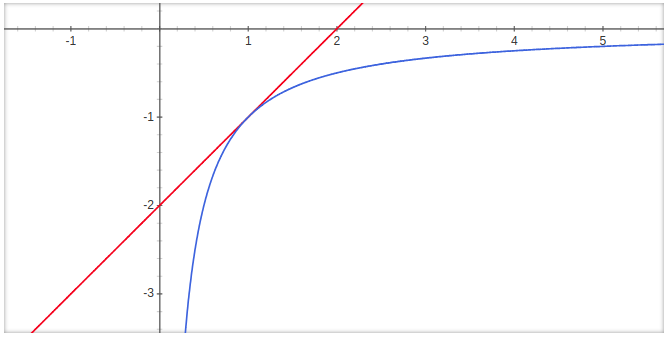
\includegraphics[width=0.49\textwidth]{derivata_00.png}\hfill%
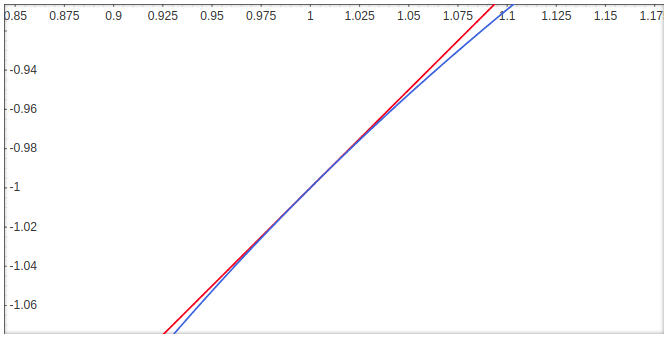
\includegraphics[width=0.49\textwidth]{derivata_01.png}
\label{fig:derivata}
\caption{Il grafico del potenziale gravitazionale terrestre.
Sull'asse delle $x$ la distanza dal centro della terra in raggi terrestri.
Sull'asse delle $y$ il potenziale gravitazionale con unità $C=GM/R$.
La pendenza della retta tangente al grafico della curva per $x=R$ è $g=GM/R^2$.
Nella figura di destra un ingrandimento in un intorno del raggio terrestre:
si nota come il grafico del potenziale risulta quasi indistinguibile dal
grafico della retta tangente.}
\end{figure}

Quello che abbiamo fatto è un procedimento di \emph{linearizzazione}%
\mymargin{linearizzazione}%
\index{linearizzazione}. 
Il campo gravitazionale è descritto da una funzione non lineare: $-GM/r$.
Ma quando ci restringiamo a un piccolo intervallo di valori di $r$ 
(i valori di $r$ vicini ad $R$, il raggio della terra) tale funzione 
risulta quasi indistinguibile, a meno di una costante, dalla funzione 
lineare $gh$ se $r=R+h$.
Le funzioni lineari sono molto più semplici da trattare ed è quindi conveniente, 
se rimaniamo sulla superficie terrestre, utilizzare quest'ultima formula per 
il potenziale gravitazionale.
Il grafico della funzione lineare che meglio approssima il grafico di una 
funzione si chiama \emph{retta tangente}%
\mymargin{retta tangente}%
\index{retta!tangente}. 
Il suo coefficiente angolare, $g$ nel nostro esempio, si chiama \emph{derivata}%
\mymargin{derivata}%
\index{derivata}.

Una volta introdotte le derivate vedremo che quello che abbiamo
determinato è la formula:
\[
U(R+h) = U(R) + U'(R) h + \omega(h).
\]

\begin{definition}[derivata]
\mymark{***}%
Sia $A\subset \RR$, $f\colon A \to \RR$, $x_0$ un punto di accumulazione di $A$.
Diremo che la funzione $f$ è \emph{derivabile} nel punto $x_0$ se esiste
ed è finito il limite:
\[
  \lim_{h\to 0} \frac{f(x_0+h) - f(x_0)}{h}.
\]
In tal caso denoteremo con $f'(x_0)$ il valore di tale limite che chiameremo
\emph{derivata}%
\mymargin{derivata}%
\index{derivata} della funzione $f$ nel punto $x_0$.

Se $B$ è l'insieme dei punti di accumulazione di $A$ in cui $f$ risulta essere derivabile, risulta quindi definita la funzione derivata $f'\colon B \to \RR$.

Una funzione $f$ si dice essere derivabile se è derivabile in ogni punto del suo dominio.
Se $C\subset A$ la funzione $f$ si dice essere \emph{derivabile su $C$} se è derivabile in ogni punto dell'insieme $C$ (cioè se $C\subset B$).

Notazioni alternative per denotare la derivata di una funzione:
\[
  f' = Df = \frac{d}{dx} f = \frac{df}{dx}.
\]
\end{definition}

Il rapporto
\[
\frac{f(x_0+h) - f(x_0)}{h}
\]
si chiama \emph{rapporto incrementale}%
\mymargin{rapporto incrementale}%
\index{rapporto!incrementale}. In effetti cambiando variabile e ponendo $x=x_0+h$ si può scrivere
\[
\frac{f(x_0+h) - f(x_0)}{h}
= \frac{f(x) - f(x_0)}{x-x_0}
= \frac{\Delta f}{\Delta x}
\]
che risulta essere il rapporto dell'incremento della funzione $f$ (a volte denotato con $\Delta f$) rispetto all'incremento corrispondente della variabile $x$ (a volte denotato con $\Delta x$).
Cambiando variabile nel limite, per $h\to 0$ si avrà $x\to x_0$
e quindi
\[
 f'(x_0) = \lim_{x\to x_0} \frac{f(x)-f(x_0)}{x-x_0}.
\]

\begin{example}
\mymark{**}
Si consideri la funzione $f(x) = 1/x$ definita sull'insieme $A = \RR \setminus \ENCLOSE{0}$. Si ha allora per ogni $x\neq 0$:
\[
  f'(x) = \lim_{h\to 0} \frac{\frac{1}{x+h} - \frac{1}{x}}{h}
        = \lim_{h\to 0} \frac{x - (x+h)}{h(x+h)x}
        = \lim_{h\to 0} \frac{-1}{(x+h)x} = -\frac{1}{x^2}.
\]
Risulta quindi che la funzione $1/x$ sia derivabile e la sua derivata è la funzione $-1/x^2$.
\end{example}

\begin{theorem}[continuità delle funzioni derivabili]
\mymark{***}
Se $f$ è derivabile nel punto $x$ allora $f$ è anche continua nel punto $x$.
\end{theorem}
%
\begin{proof}
\mymark{***}
Si ha
\[
  \lim_{h\to 0} f(x+h) - f(x) = \lim_{h\to 0} \frac{f(x+h) - f(x)}{h} \cdot h
  = f'(x) \cdot 0 = 0.
\]
Dunque $f(x+h)\to f(x)$ per $h\to 0$ e quindi $f$ è continua nel punto $x$.
\end{proof}

\begin{example}[funzione continua ma non derivabile]
\mymark{***}
La funzione $f(x) = \abs{x}$ è un esempio di funzione continua ma non
derivabile. E' infatti facile verificare che nel punto $x_0=0$ il
limite destro del rapporto incrementale è $1$ mentre il limite
sinistro è $-1$.

Un altro esempio è la funzione $f(x) = \sqrt{x}$ che è continua ma non
è derivabile nel punto $x_0=0$ perché il limite del rapporto incrementale esiste ma è $+\infty$.
\end{example}



\begin{theorem}[derivata della funzione composta]
\mymark{**}
Sia $f$ una funzione derivabile nel punto $x_0$
e sia $g$ una funzione derivabile nel punto $f(x_0)$.
Allora la funzione composta $g\circ f$ è derivabile
nel punto $x_0$ e si ha:
\[
  (g\circ f)'(x_0) = g'(f(x_0))\cdot f'(x_0).
\]
\end{theorem}
%
\begin{proof}
\mymark{**}
Consideriamo la funzione
\[
  G(y) =
  \begin{cases}
   \frac{g(y) - g(f(x_0))}{y-f(x_0)} & \text{se $y \neq f(x_0)$},\\
   g'(f(x_0)) & \text{se $y=f(x_0)$}.
  \end{cases}
\]
Si avrà allora
\begin{equation}\label{eq:47439}
 \frac{g(f(x_0+h))-g(f(x_0))}{h}
 = G(f(x_0+h)) \cdot \frac{f(x_0+h)-f(x_0)}{h}
\end{equation}
infatti se $f(x_0+h)\neq f(x_0)$ abbiamo moltiplicato e diviso
per $f(x_0+h) - f(x_0)$ se invece $f(x_0+h)=f(x_0)$ allora anche $g(f(x_0+h))=g(f(x_0))$ e l'uguaglianza è ancora valida perché sia il lato sinistro che il lato destro si annullano (e il valore assegnato a $G$ risulta in tal caso irrilevante).

Chiaramente quando $h\to 0$ il secondo fattore sul lato destro
dell'uguaglianza \eqref{eq:47439}
tende, per definizione, a $f'(x_0)$.
Per quanto riguarda il primo fattore
osserviamo che $G(y)$, per come è stata definita, risulta essere una funzione continua nel punto $y=f(x_0)$ in quanto
\[
\frac{g(y) - g(f(x_0))}{y-f(x_0)} \to g'(f(x_0))
\]
per $y\to f(x_0)$.
Ma anche la funzione $f$ è continua nel punto $x_0$ (in quanto derivabile).
Dunque la funzione composta $G(f(x_0+h))$ è continua nel punto $h=0$.
Risulta quindi che $G(f(x_0+h)) \to G(f(x_0)) = g'(f(x_0))$ per $h\to 0$.
Dunque il lato destro di \eqref{eq:47439} ha limite $g'(f(x_0)) \cdot f'(x_0)$ per $h\to 0$, come volevamo dimostrare.
\end{proof}

\begin{theorem}[derivata della funzione inversa]
\mymark{**}
Sia $f$ una funzione invertibile derivabile in un punto $x_0$ e
supponiamo che la funzione inversa $f^{-1}$ sia continua in $f(x_0)$.
Se $f'(x_0)\neq 0$ allora $f^{-1}$ è derivabile in $f(x_0)$ e vale:
\[
  (f^{-1})'(f(x_0)) = \frac{1}{f'(x_0)}.
\]
Chiamato $y_0 = f(x_0)$ la formula può essere anche scritta nella forma:
\[
  (f^{-1})'(y_0) = \frac{1}{f'(f^{-1}(y_0))}.
\]
Se invece $f'(x_0)=0$ la funzione $f^{-1}$ non è derivabile in $f(x_0)$.
\end{theorem}
%
Osserviamo che se $f$ è definita in un intervallo e se è invertibile e
continua in tutto l'intervallo allora certamente l'inversa è continua
(Esercizio~\ref{ex:inversa_monotona}).
%
\begin{proof}
\mymark{**}
Posto $y_0 = f(x_0)$ consideriamo il rapporto incrementale di $f^{-1}$ nel punto $y_0$:
\[
  \frac{f^{-1}(y) - f^{-1}(y_0)}{y-y_0}.
\]
Per $y\to y_0$ possiamo fare il cambio di variabile
$x=f^{-1}(y)$ in quanto avendo assunto che $f^{-1}$ sia continua in $f(x_0)$ sappiamo che se $y\to y_0$ allora $x = f^{-1}(y)\to f^{-1}(y_0) = x_0$.
Si ha allora per $y\to y_0$ che $x\to x_0$ e,
se $f'(x_0)\neq 0$:
\[
  \frac{f^{-1}(y) - f^{-1}(y_0)}{y-y_0}
  = \frac{x-x_0}{f(x)-f(x_0)}
  = \frac{1}{\frac{f(x)-f(x_0)}{x-x_0}} \to \frac{1}{f'(x_0)}.
\]

Se invece $f'(x_0)=0$ il rapporto incrementale della funzione inversa
ha limite infinito e quindi la funzione inversa non è derivabile in $f(x_0)$.
\end{proof}


\begin{theorem}[operazioni con le derivate]
\mymark{***}
Siano $f$ e $g$ due funzioni derivabili in uno stesso punto $x_0$.
Allora le funzioni $f+g$, $f-g$, $f\cdot g$ e, se $g(x_0)\neq 0$ anche $f/g$ sono funzioni derivabili in $x_0$. Nei punti in cui entrambe le funzioni sono derivabili si ha
\begin{gather*}
  (f+g)' = f' + g', \qquad
  (f-g)' = f' - g', \\
  (f\cdot g)' = f' \cdot g + f g', \qquad
  \enclose{\frac{f}{g}}' = \frac{f'g - fg'}{g^2}.
\end{gather*}
\end{theorem}
%
\begin{proof}
\mymark{***}
Per quanto riguarda la derivata della somma (o della differenza) è sufficiente osservare che il rapporto incrementale della somma (o della differenza) è la somma (o la differenza) dei rapporti incrementali e che il limite della somma (o della differenza) è uguale alla somma (o la differenza) dei limiti.

Calcoliamo la derivata del prodotto $f\cdot g$ nel punto $x_0$. Si ha
\begin{align*}
  \frac{f(x)g(x) - f(x_0)g(x_0)}{x-x_0}
  &= \frac{f(x)(g(x) - g(x_0)) + (f(x)-f(x_0))g(x_0)}{x-x_0}\\
  &= f(x) \frac{g(x)-g(x_0)}{x-x_0} + \frac{f(x)-f(x_0)}{x-x_0} g(x_0).
\end{align*}
Passando al limite per $x\to x_0$ ci ricordiamo che $f(x)\to f(x_0)$ in quanto $f$ è continua in $x_0$ (essendo per ipotesi derivabile). I rapporti incrementali tendono alle derivate e si ottiene quindi il risultato voluto $f(x_0) g'(x_0) + f'(x_0) g(x_0)$.

Per quanto riguarda la derivata del rapporto osserviamo che
posto $h(y)=1/y$ si ha
\[
  \frac{f(x)}{g(x)} = f(x) \cdot h(g(x)).
\]
Dall'esercizio già svolto sappiamo che $h'(y) = -1/y^2$ e dunque
possiamo utilizzare le formule per la derivata del prodotto e la derivata della funzione composta per ottenere:
\begin{align*}
  \enclose{\frac{f}{g}}'(x_0)
  &= \enclose{f \cdot (g\circ h)}'(x_0) \\
  &= f'(x_0) \cdot h(g(x_0)) + f(x_0) \cdot h'(g(x_0))\cdot g'(x_0)\\
  &= \frac{f'(x_0)}{g(x_0)} + f(x_0) \cdot \frac{-1}{g^2(x_0)} g'(x_0)\\
  &= \frac{f'(x_0)g(x_0) - f(x_0)g'(x_0)}{g^2(x_0)}.
\end{align*}
\end{proof}

\begin{table}
  \begin{tabular}{c|c||c|c||c|c}
    $f(x)$ & $f'(x)$ & $f(x)$ & $f'(x)$ & $f(x)$ & $f'(x)$
    \\\hline
    $mx + q$ & $m$ &
    $e^x$ & $e^x$ &
    $\sin x$ & $\cos x$ \\
    $\abs{x}$ & $\frac{x}{\abs{x}}$ &
    $\ln x$ & $\frac 1 x$ &
    $\cos x$ & $-\sin x$ \\
    $x^n$ & $n x^{n-1}$ &
    $\sinh x$ & $\cosh x$ &
    $\arcsin x$ & $\frac{1}{\sqrt{1-x^2}}$ \\
    $x^\alpha$ & $\alpha x^{\alpha -1}$ &
    $\cosh x$ & $\sinh x$ & $\arccos x$ & $-\frac{1}{\sqrt{1-x^2}}$ \\
    $\sqrt[n]{x}$ & $\frac{1}{n\sqrt[n]{x^{n-1}}}$ &
    $\settsinh x$ & $\frac{1}{\sqrt{x^2+1}}$ &
    $\tg x$ & $1+ \tg^2 x$ \\
    $\sqrt{x}$ & $\frac{1}{2\sqrt{x}}$ &
    $\settcosh x$ & $\frac{1}{\sqrt{x^2-1}}$ &
    $\arctg x$ & $\frac{1}{1+x^2}$
  \end{tabular}
  \caption{Derivate delle funzioni elementari}
  \label{tab:derivate}%
\end{table}

\begin{theorem}[derivate delle funzioni elementari]%
\label{th:derivate_elementari}%
\index{derivata!delle funzioni elementari}%
\mymark{**}%
Per $m,q,\alpha \in \RR$, $\alpha \neq 0$, $n\in \NN$, $n\neq 0$
valgono le regole di derivazione riassunte nella
tabella~\ref{tab:derivate}: le funzioni nella colonna
$f(x)$ hanno la derivata riportata nella colonna $f'(x)$.
Le funzioni $f(x)$ sono derivabili nei punti in cui la
corrispondente espressione $f'(x)$ è ben definita.
In particolare:
la funzione $\sqrt[n]{x}$
non è derivabile in $x=0$,
le funzioni $\arcsin x$ e $\arccos x$ non sono derivabili nei punti $-1$ e $1$,
la funzione $\abs{x}$ non è derivabile in $0$,
la funzione $\settcosh x$ non è derivabile in $1$.
Le funzioni lineari, potenze con base positiva, potenze con esponente intero,
esponenziale, logaritmo, seno, coseno, tangente, arcotangente sono invece derivabili
in tutti i punti in cui sono definite.
\end{theorem}

\begin{proof}
\mymark{**}
Per quanto riguarda le funzioni lineari si ha:
\begin{align*}
(mx+q)' &= \lim_{h\to 0}\frac{m(x+h)+q - (mx+q)}{h} = \lim_{h\to 0} m = m.
\end{align*}
Ricordando che la derivata è un limite e che il limite in un punto dipende 
solo dai valori della funzione in un intorno del punto, 
possiamo affermare che la derivata del valore assoluto $\abs{x}$ 
coincide con la derivata di $x$ cioè $1$ sugli $x>0$ e coincide 
con la derivata di $-x$ sugli $x<0$. Dunque $D \abs{x} = x / \abs{x}$ 
se $x\neq 0$. 
Se $x=0$ i limiti destro e sinistro del rapporto incrementale di $\abs{x}$ 
tendono rispettivamente a $1$ e $-1$ e quindi la derivata non esiste.

Dimostriamo che $Dx^n = n D x^{n-1}$ per $n\in \NN$, $n>0$, 
per induzione su $n$. Per $n=1$ abbiamo $x^n=x^1$ è lineare 
e quindi dalla formula precedente $Dx^1 = 1 = 1 \cdot x^0$. 
Supponendo di sapere che $D x^n = n x^{n-1}$ si ha, applicando 
la regola di derivazione del prodotto:
\[
  D x^{n+1} = D x\cdot x^n = 1 \cdot x^n + x \cdot n x^{n-1}
   = x^n + n x^n = (n+1) x^n
\]
dimostrando dunque il passo induttivo.
Ricordando la formula di derivazione del rapporto
possiamo trovare la formula per le potenze con esponente intero negativo:
\[
  D x^{-n} = D \frac{1}{x^n} = \frac{-n x^{n-1}}{x^{2n}}
   = -n x^{n-1-2n} = -n x^{-n-1}.
\]

La derivata della radice $n$-esima si trova con la formula di derivazione della funzione inversa $x^n$, che può essere applicata se $x\neq 0$:
\[
  D \sqrt[n]{x} = \frac{1}{n(\sqrt[n]{x})^{n-1}}
    = \frac{1}{n\sqrt[n]{x^{n-1}}}.
\]
Osserviamo che se $n$ è dispari la formula è valida anche per $x<0$.
La derivata della radice quadrata si ottiene ponendo $n=2$.

Per quanto riguarda la derivata dell'esponenziale
ci riconduciamo ad un limite notevole:
\[
  D e^x = \lim_{h\to 0} \frac{e^{x+h}-e^x}{h}
  = \lim_{h\to 0}\frac{e^x e^h - e^x}{h}
  = \lim_{h\to 0}e^x \frac{e^h - 1}{h}
  = e^x.
\]
La derivata del logaritmo si ottiene come derivata della funzione inversa dell'esponenziale:
\[
  D \ln x = \frac{1}{e^{\ln x}} = \frac{1}{x}.
\]
Possiamo quindi calcolare la derivata delle potenze con base positiva e esponente reale qualunque:
\[
D x^\alpha
= D e^{\alpha \ln x}
= e^{\alpha \ln x} D(\alpha \ln x)
= x^\alpha \alpha \frac{1}{x}
= \alpha x^{\alpha -1}.
\]

Per quanto riguarda le funzioni trigonometriche $\sin$ e $\cos$ ci ricordiamo dei limiti notevoli:
\[
  \lim_{h\to 0}\frac{\sin h}{h} = 1,\qquad
  \lim_{h\to 0}\frac{1-\cos h}{h}
  =\lim_{h\to 0}h \cdot \frac{1-\cos h}{h^2} = 0 \cdot \frac{1}{2} = 0.
\]
Applicando le formule di addizione si ha
\begin{align*}
  D \sin x
  &= \lim_{h\to 0}\frac{\sin(x+h)-\sin(x)}{h} \\
  &= \lim_{h\to 0}\frac{\sin(x)\cos(h) + \cos(x)\sin(h) - \sin(x)}{h} \\
  &= \lim_{h\to 0}\sin(x) \frac{\cos h-1}{h} + \cos(x) \frac{\sin h}{h} = \cos(x).
\end{align*}
e similmente
\begin{align*}
  D \cos x
  &= \lim_{h\to 0}\frac{\cos(x+h)-\cos(x)}{h} \\
  &= \lim_{h\to 0}\frac{\cos(x)\cos(h) - \sin(x)\sin(h) - \cos(x)}{h} \\
  &= \lim_{h\to 0}\cos(x) \frac{\cos h-1}{h} - \sin(x) \frac{\sin h}{h} = -\sin(x)
\end{align*}

La funzioni $\arcsin$ è definita come l'inversa della restrizione della funzione $\sin$ all'intervallo $[-\pi/2, \pi/2]$.
Nell'intervallo aperto $(-\pi/2,$ $\pi/2)$ la funzione $\sin$ ha derivata positiva e dunque risulta che la funzione inversa (che sappiamo essere continua) è derivabile in $(-1,1)$ e la sua derivata è
\[
D\arcsin x
= \frac{1}{\cos(\arcsin x)}
= \frac{1}{\sqrt{1-\sin^2 \arcsin x}}
= \frac{1}{\sqrt{1-x^2}}.
\]
Si ha infatti $\cos y = \sqrt{1-\sin^2 y}$ se $y\in [-\pi/2, \pi/2]$.

Analogamente la funzione $\arccos$ è definita come l'inversa della restrizione di $\cos$ all'intervallo $[0,\pi]$ e si ha quindi,
per $x\in (-1,1)$
\[
D \arccos x
 = \frac{1}{-\sin(\arccos x)}
 = \frac{1}{-\sqrt{1-\cos^2 \arccos x}}
 = -\frac{1}{\sqrt{1-x^2}}.
\]
Si ha infatti $\sin y = \sqrt{1-\cos^2 y}$ se $y\in[0,\pi]$.

Nei punti $x=1$ e $x=-1$ le funzioni $\arcsin$ e $\arccos$ non sono invece derivabili.

Per la funzione tangente possiamo utilizzare la formula di derivazione del rapporto:
\begin{align*}
  D \tg x &= D \frac{\sin x }{\cos x}
   = \frac{\cos x \cdot \cos x - \sin x \cdot (-\sin x)}{\cos^2 x} \\
   &= \frac{\cos^2 x + \sin^2 x}{\cos^2 x}
   = 1 + \tg^2 x = \frac{1}{\cos^2 x}.
\end{align*}
Usando la formula della derivata della funzione inversa si ha
\[
  D \arctg x = \frac{1}{1+\tg^2(\arctg x)}
  = \frac{1}{1+x^2}.
\]

Per quanto riguarda le funzioni iperboliche le derivate di $\sinh$
e $\cosh$ si riconducono immediatamente alla derivata dell'esponenziale,
utilizzando
la definizione~\eqref{eq:sinh_cosh}. Le derivate delle funzioni
inverse $\settsinh$ e $\settcosh$ si ottengono dalla formula per la derivata
della funzione inversa e utilizzando
le relazioni $\cosh x = \sqrt{\sinh^2 x+1}$ e, per $x > 0$,
$\sinh x = \sqrt{\cosh^2 x -1}$:
\begin{align*}
  D \settsinh x &= \frac{1}{\cosh(\settsinh x)}
  = \frac{1}{\sqrt{\sinh^2 (\settsinh x) + 1}} = \frac{1}{\sqrt{x^2+1}}\\
  D \settcosh x &= \frac{1}{\sinh(\settcosh x)}
  = \frac{1}{\sqrt{\cosh^2(\settcosh x)-1}}
  = \frac{1}{\sqrt{x^2-1}}
\end{align*}
\end{proof}

\begin{proposition}[trucco di Feynman per le derivate]
  \index{trucco!di Feynman}%
  \index{trucco!di Feynman!per le derivate}%
  \index{Feynman!trucco per le derivate}%
Siano $f_1,\dots, f_n$ funzioni derivabili e siano $\alpha_1,\dots, \alpha_n$ 
esponenti reali. Allora:
  \[
  \enclose{\prod_{k=1}^n f_k^{\alpha_k}}'
  = \prod_{k=1}^n f_k^{\alpha_k} \cdot \sum_{k=1}^n \alpha_k \frac{f_k'}{f_k}.
  \]
\end{proposition}
\begin{proof}
Basta osservare che 
\begin{align*}
  \enclose{\prod_{k=1}^n f_k^{\alpha_k}}'
  &= \sum_{k=1}^n \alpha_k f_k' f_k^{\alpha_k-1} \prod_{j\neq k} f_j^{\alpha_j}
  = \sum_{k=1}^n \alpha_k \frac{f_k'}{f_k} \prod_{j=1}^n f_j^{\alpha_j}.
\end{align*}
\end{proof}
Se ad esempio vogliamo calcolare la derivata della funzione 
\[
 \frac{\sqrt{1-x^2}\cdot \ln x}{x\cdot \cos^2 x}
 = (1-x^2)^{\frac 1 2} \cdot \ln x \cdot x^{-1}\cdot (\cos x)^{-2}
\]
otteniamo 
\[
  \frac{\sqrt{1-x^2}\cdot \ln x}{x\cdot \sin^2 x}
  \cdot \Enclose{\frac 1 2 \cdot \frac{-2x}{1-x^2} + \frac{1}{x\ln x} - \frac{1}{x}-2\frac{-\sin x}{\cos x}}.
\]

\section{derivate parziali}

Capita a volte di avere funzioni che dipendono da più variabili o da parametri.
Ad esempio la funzione $f(x,y) = x^2y+y^2$ è una funzione definita 
sulle coppie di numeri reali: $f\colon \RR^2\to \RR$.
Se considero una delle due variabili, ad esempio la prima variabile $x$, 
come un parametro fissato, posso identificare la funzione $f$ come 
una funzione $g\colon \RR \to (\RR^\RR)$ 
che ad ogni valore del parametro $x$ restituisce una funzione 
della variabile $y$:
\[
  g(x)(y) = f(x,y).
\]
Dunque per ogni $x$ fissato, posso considerare la funzione $h=g(x)$
che è una funzione della sola variabile $y$: $h(y) = g(x)(y) = f(x,y)$.  
E posso quindi farne la derivata $h'(y)$ in qualunque punto $y$. 
Il valore che ottengo si chiama \emph{derivata parziale}%
\mymargin{derivata parziale}%
\index{derivata!parziale}
della funzione $f$ rispetto alla variabile $y$ calcolata nel punto $(x,y)$.
Per fare il calcolo della derivata possiamo applicare le usuali regole di 
derivazione facendo attenzione che se stiamo 
facendo la derivata rispetto a $y$ la variabile $x$ va trattata come se 
fosse costante, perché stiamo in effetti fissando $x$ prima di fare la derivata.
Se $f(x,y) = x^2y+y^2$ si ottiene dunque%
\mynote{Se non siamo abituati a pensare che $x$ possa essere un valore fissato 
si provi a sostituire la variabile $x$ con una lettera diversa come $c$ o $\pi$ che ci dà l'idea 
di una quantità costante.}:
$h'(y) = x^2 + 2y$.
Se ora consideriamo anche $x$ variabile otteniamo una nuova funzione di due 
variabili $(x,y)\mapsto g(x)'(y) = h'(y)$ che può essere scritta 
con le seguenti notazioni% 
\mynote{%
Si osservi che per le funzioni di più variabili c'è una ambiguità di fondo nelle notazioni.
Infatti se ho una espressione in due variabili come $x^2 y + y^2$ è chiaro 
che questa rappresenta una funzione di due variabili ma non è del tutto ovvio dire quale 
è la prima variabile e quale è la seconda. 
Normalmente le variabili vengono indicate in ordine alfabetico a partire dalla $x$... 
ma è solo una convenzione. In principio l'espressione $x^2y + y^2$ 
potrebbe anche rappresentare una funzione di tre variabili $x,y,z$. 
Dunque se ho una espressione che utilizza certi nomi per le variabili è naturale 
usare gli stessi nomi nel simbolo utilizzato per la derivata parziale come 
nella notazione $D_y$.
Se invece le variabili non hanno un nome sarebbe più sensato indicare la variabile dandone 
la posizione numerica come nella notazione $D_2$.
Ci sono casi in cui la notazione può essere molto ambigua, come ad esempio 
se scrivessi $\frac{\partial f(y,x)}{\partial y}$: 
sto derivando $f$ rispetto alla prima variabile oppure derivo $f(x,y)$ rispetto alla seconda 
variabile e poi scambio le due variabili?
}:
\begin{align*}
\frac{\partial f(x,y)}{\partial y} 
&= \frac{\partial f}{\partial y}(x,y)
= D_y f(x,y)
= f_y (x,y) \\
&= D_2 f(x,y) = f_{,2} (x,y) \\
&= h'(y)
\end{align*}

Analogamente potremmo fare la derivata parziale di $f$ rispetto alla prima 
variabile $x$. Se $f(x,y) = x^2y+y^2$ si ottiene
\[
\frac{\partial f(x,y)}{\partial x} = 2xy.
\]

Stiamo qui trattando le funzioni di più variabili come se fossero funzioni di una sola 
variabile dipendenti da altri parametri. 
Questo perché stiamo facendo un corso di analisi sulle funzioni di \emph{una} variabile (reale).
\index{una!variabile}%
\index{funzione!di una variabile}%
\index{variabile!funzione di una}%
Per trattare tutte le variabili come una unica variabile multidimensionale 
bisogna fare diverse considerazioni 
aggiuntive che vengono trattate nei corsi di analisi sulle funzioni di 
\emph{più} 
\index{più!variabili}%
\index{funzione!di più variabili}%
\index{variabili!funzione di più}%
variabili (reali). 
Verranno in tal caso introdotti i concetti di \emph{gradiente} $\nabla f$, 
\emph{derivata} $Df$ e \emph{differenziale} $df$ che noi non affronteremo qui.

\section{punti notevoli}

In questa sezione introdurremo una terminologia che è largamente utilizzata 
nello studio di funzione.
Cercheremo di dare delle definizioni anche per alcuni termini su cui potrebbe 
non esserci un consenso univoco.
Ricordiamoci di non usare queste definizioni in modo troppo formale:
sarà sempre meglio
verificare che il nostro interlocutore ci comprenda
perché spesso alcuni termini potrebbero essere utilizzati in maniera
impropria o con significati leggermente diversi.

Nel dubbio potremo sempre evitare di utilizzare questa terminologia 
riconducendoci ai concetti sottostanti.

\begin{definition}[punti notevoli]
Sia $f\colon A \subset \RR \to \RR$ una funzione. Se $f$ è derivabile in un
punto $x_0\in A$ e $f'(x_0) = 0$ diremo che $x_0$ è un \emph{punto critico}%
\mymargin{punto critico}%
\index{punto!critico}
o
\emph{punto stazionario}
\index{punto!stazionario}
di $f$.

Se $x_0\in A$ ed esiste un intorno $U$ di $x_0$ per cui $x_0$ risulta
essere un punto di minimo (rispettivamente di massimo) per $f$ ristretta ad $U$
diremo che $x_0$ è un punto di \emph{minimo relativo}%
\mymargin{minimo relativo}%
\index{minimo!relativo} o \emph{minimo locale}
(rispettivamente \emph{massimo relativo} o \emph{massimo locale}).
Per contrapposizione i punti di massimo e minimo su tutto il dominio $A$
vengono anche
chiamati massimo/minimo \emph{assoluto} di $f$.

Diremo che $x_0\in A$ è un \emph{punto di flesso}%
\mymargin{punto di flesso}%
\index{punto!di flesso} per $f$ se
$f$ è derivabile in un intorno di $x_0$ e $x_0$ è un punto di massimo
o minimo relativo per $f'$. Nel punto $x_0$ la retta tangente
ha equazione $y=r(x) = f'(x_0) (x-x_0) + f(x_0)$. Se $x_0$ è
minimo per $f'$ risulta che $f(x)-r(x)$ è crescente
quindi $f(x)\ge r(x)$ per $x\ge x_0$ e $f(x)\le r(x)$ per $x\le x_0$
(il grafico della funzione attraversa la retta tangente da sotto a sopra)
mentre se $x_0$ è massimo per $f'$ risulta che $f(x)\le r(x)$ per $x\ge x_0$
e $f(x) \ge r(x)$ per $x\le x_0$ (il grafico della funzione attraversa
la tangente da sopra a sotto).
Se la funzione $f$ non è derivabile in $x_0$ ma il limite del rapporto
incrementale esiste ed è infinito, diremo che $x_0$ è un
\emph{flesso verticale}%
\mymargin{flesso verticale}%
\index{flesso!verticale}. In tale punto la retta tangente è verticale
e il grafico della funzione attraversa tale retta.

Sia $x_0\in A$ un punto in cui la funzione $f$ è continua ed esistono
i limiti destro e sinistro del rapporto incrementale
(che si chiamano \emph{derivata destra} e \emph{derivata sinistra})
\[
  m^{\pm} = \lim_{h\to 0^\pm}\frac{f(x+h) - f(x)}{h}.
\]
Se $m^+ \neq m^-$ chiaramente $f$ non è derivabile in $x_0$.
Se entrambi $m^+$ ed $m^-$ sono finiti diremo che $x_0$ è un
\emph{punto angoloso}%
\mymargin{punto angoloso}%
\index{punto!angoloso} in quanto le due semirette tangenti
in $x_0$ (da destra e da sinistra) formano un angolo non piatto.
Se $m^+=-m^-=+\infty$ oppure se $m^+=-m^-=-\infty$
diremo che il punto $x_0$ è un \emph{punto di cuspide}%
\mymargin{punto di cuspide}%
\index{punto!di cuspide} (c'è una
semiretta tangente verticale).
\end{definition}

\begin{definition}[asintoti]
Diremo che la retta $y=mx+q$ è un asintoto per il grafico di $f$ 
per $x\to +\infty$ se risulta
\[
  \lim_{x\to +\infty} f(x) - (mx+q) = 0.
\]
Se $m=0$ diremo che il grafico di $f$ ha un \emph{asintoto orizzontale} $y=q$
\mymargin{asintoto orizzontale e obliquo}%
\index{asintoto orizzontale e obliquo}%
\index{asintoto!orizzontale}%
\index{asintoto!obliquo}%
altrimenti diremo che $y=mx+q$ è un \emph{asintoto obliquo}.
Stessa cosa si può dire per $x\to -\infty$.

Se $x_0\in \RR$ e si ha 
\[
  \lim_{x\to x_0} \abs{f(x)} = +\infty
\]
diremo che la retta $x=x_0$ è un \emph{asintoto verticale}%
\mymargin{asintoto verticale}%
\index{asintoto!verticale} per il 
grafico della funzione $f$.
\end{definition}

\begin{definition}[punti di discontinuità]
Se per $x_0\in \RR$ si ha 
\[
  \lim_{x\to x_0^-} f(x) = \ell_1, 
  \qquad 
  \lim_{x\to x_0^+} f(x) = \ell_2
\]
e se $\ell_1\neq \ell_2$ diremo che nel punto $x_0$ 
la funzione $f$ ha una \emph{discontinuità a salto}%
\mymargin{discontinuità a salto}%
\index{discontinuità!a salto}.
Se $\ell_1=\ell_2$ e se $f$ non è definita nel punto $x_0$ 
oppure se $f(x_0)\neq \ell_1$ diremo che 
nel punto $x_0$ la funzione $f$ 
ha una \emph{discontinuità eliminabile}%
\mymargin{discontinuità eliminabile}%
\index{discontinuità!eliminabile}.
\end{definition}

Si osservi che, nonostante la terminologia utilizzata,
una funzione continua può avere una discontinuità 
a salto (ad esempio: $f(x)=\frac{x}{\abs{x}}$) 
e può anche avere una discontinuità eliminabile
(ad esempio: $f(x) = \frac{x}{x}$).

\section{criteri di monotonia}

\begin{theorem}[Fermat]
\mymark{***}
Sia $f\colon (a,b)\to \RR$ una funzione derivabile.
Se $x_0\in (a,b)$ è un punto di massimo o minimo per $f$ allora
$f'(x_0)=0$.
\end{theorem}
%
\begin{proof}
\mymark{***}
Senza perdere di generalità possiamo suppore che $x_0$ sia un punto di massimo per $f$.
Sappiamo che
\[
  f'(x_0) = \lim_{x\to x_0}\frac{f(x)-f(x_0)}{x-x_0}.
\]
Visto che $x_0$ è un punto dell'intervallo aperto $(a,b)$ la funzione $f$ è definita in un intorno destro di $x_0$ e quindi possiamo restingere il limite ai valori $x>x_0$ ottenendo:
\[
  f'(x_0) = \lim_{x\to x_0^+}\frac{f(x) - f(x_0)}{x-x_0}.
\]
Visto che $x_0$ è un punto di massimo per $f$ sappiamo che $f(x)-f(x_0)\le 0$. Essendo $x-x_0>0$ l'intero rapporto incrementale risulta essere non positivo.
Dunque, per il teorema della permanenza del segno,
possiamo concludere che $f'(x_0)\le 0$.

Ma possiamo anche restringere la funzione ad un intorno sinistro di $x_0$ e osservare che
\[
  f'(x_0) = \lim_{x\to x_0^-}\frac{f(x)-f(x_0)}{x-x_0}.
\]
Ma ora il numeratore è, come prima, non positivo mentre il denominatore $x-x_0$ è negativo. Dunque il rapporto incrementale stavolta è non negativo e quindi, per la permanenza del segno, $f'(x_0) \ge 0$.

Abbiamo scoperto quindi che $f'(x_0)\le 0$ e $f'(x_0)\ge 0$
da cui deduciamo $f'(x_0)=0$.
\end{proof}

Il teorema di Fermat si può
enunciare dicendo che ogni punto di massimo o minimo relativo interno
al dominio di una funzione in cui la funzione è derivabile
è necessariamente un punto critico.
In particolare per determinare massimi e minimi assoluti e relativi
di una funzione sarà sufficiente esaminare i punti di frontiera,
i punti di non derivabilità e i punti critici.


\begin{theorem}[Rolle]
\mymark{***}
\index{teorema!di Rolle}
\mymargin{Rolle}%
\index{Rolle}
Sia $f\colon [a,b]\to \RR$, $a,b\in \RR$, $a<b$, una funzione continua su tutto $[a,b]$ e derivabile su $(a,b)$.
\mynote{Se $b<a$ il teorema è ugualmente valido 
se si intende $[a,b]=[b,a]$}%
Se $f(a) = f(b)$ allora esiste $x_0 \in (a,b)$ tale che $f'(x_0)=0$.
\end{theorem}
%
\begin{proof}
\mymark{***}
Essendo $f$ una funzione continua
possiamo applicare il teorema di Weiestrass per dedurre che $f$ ha massimo e 
minimo sull'intervallo chiuso e limitato $[a,b]$. 
Se il punto di massimo o il punto di minimo sta nell'intervallo aperto 
$(a,b)$ possiamo applicare il teorema di Fermat per ottenere che la derivata 
di $f$ si annulla in tale punto.

In caso contrario sia il punto di massimo che il punto di minimo sono estremi 
dell'intervallo, cioè sono uguali ad $a$ o a $b$. Ma visto che $f(a)=f(b)$ 
i valori massimo e minimo coincidono e quindi la funzione è costante. 
Ma in tal caso $f'(x)=0$ per ogni $x\in [a,b]$.
\end{proof}

\begin{theorem}[Lagrange]\label{th:lagrange}%
\mymark{***}%
\index{teorema!di Lagrange}%
\mymargin{Lagrange}%
\index{Lagrange}%
Sia $f\colon [a,b]\to \RR$ una funzione continua su $[a,b]$ e derivabile su $(a,b)$
con $a,b\in \RR$, $a<b$.
\mynote{Se $b<a$ il teorema è ugualmente valido 
se si intende $[a,b]=[b,a]$}%
Allora esiste un punto $x_0\in (a,b)$ tale che
\[
  f'(x_0) = \frac{f(b) - f(a)}{b-a}
\]
\end{theorem}
%
\begin{proof}
\mymark{***}
Consideriamo la funzione ausiliaria:
\[
  g(x) = f(x) - \frac{f(b)-f(a)}{b-a} x.
\]
Per verifica diretta si osserva che
\[
  g(b) = g(a) = \frac{b f(a) - a f(b)}{b-a}.
\]
La funzione $g$ soddisfa quindi le ipotesi del teorema di Rolle e dunque esisterà $x_0\in (a,b)$ tale che $g'(x_0)=0$.
Ma si osserva che
\[
  g'(x) = f'(x) - \frac{f(b)-f(a)}{b-a}
\]
e dunque se $g'(x_0)=0$ si ottiene il risultato desiderato.
\end{proof}

\begin{theorem}[criteri di monotonia]%
\label{th:criteri_monotonia}
\mymark{***}%
\mymargin{criteri di monotonia}%
\index{criterio!di monotonia}%
Sia $f\colon I \to \RR$ una funzione definita su un intervallo $I\subset \RR$. Sia $J= (\inf I, \sup I)$ l'intervallo aperto con gli stessi estremi di $I$.
Supponiamo che $f$ sia continua su $I$ e derivabile su $J$. 
Allora valgono i seguenti criteri:
\begin{enumerate}
\item
$(\forall x \in J\colon f'(x)\ge 0)$
$\iff$
$f$ è crescente (su tutto $I$);
\item
$(\forall x \in J\colon f'(x)\le 0)$
$\iff$
$f$ è decrescente (su tutto $I$);
\item
$(\forall x \in J\colon f'(x)=0)$
$\iff$
$f$ è costante (su tutto $I$);
\item
$(\forall x \in J\colon f'(x)>0)$
$\implies$
$f$ è strettamente crescente (su tutto $I$);
\item
$(\forall x \in J\colon f'(x)<0)$
$\implies$
$f$ è strettamente decrescente (su tutto $I$).
\end{enumerate}
\end{theorem}
%
\begin{proof}
\mymark{***}
Dimostriamo innanzitutto le implicazioni da sinistra verso destra.

Per la prima, se $f$ non fosse crescente ci dovrebbero essere due punti $a, b \in I$ tali che $a < b$ ma $f(a) > f(b)$.
Dunque si avrebbe
\[
  \frac{f(b) - f(a)}{b - a} < 0.
\]
Applicando il teorema di Lagrange all'intervallo $[a,b]$ si troverebbe un punto $x\in (a,b)$ tale che $f'(x) < 0$. Chiaramente $(a,b)\subset J$ e quindi questo contraddice l'ipotesi $f'(x) \ge 0$.

La seconda implicazione (per le funzioni decrescenti) si dimostra in maniera analoga cambiando verso alle disuguaglianze.

Anche la terza implicazione si dimostra tramite il teorema di Lagrange in modo analogo alle precedenti. Oppure basta osservare che se $f'(x)=0$ allora valgono contemporaneamente $f'(x)\ge 0$ e $f'(x)\le 0$ quindi mettendo insieme le prime due implicazioni si ottiene che $f$ è contemporaneamente crescente e decrescente dunque è costante.

Per la quarta implicazione si procede come per la prima. Per assurdo si  avrebbero $a<b$ con $f(b) \le f(a)$. Ma allora
\[
  \frac{f(b) - f(a)}{b-a} \le 0
\]
e applicando il teorema di Lagrange si troverebbe un punto $x\in (a,b)$ con $f'(x) \le 0$, contro l'ipotesi $f'(x) > 0$.

La quinta implicazione si dimostra in maniera analoga cambiando verso alle disuguaglianze.

Vediamo ora le implicazioni da destra verso sinistra.
Per la prima, supponiamo che $f$ sia crescente e prendiamo $x\in J$. Allora è chiaro che per ogni $h>0$ si avrà $f(x+h) \ge f(x)$ e dunque
\[
  \frac{f(x+h)- f(x)}{h} \ge 0.
\]
Facendo il limite per $h \to 0^+$ si ottiene $f'(x)$ e, per la permanenza del segno, dovra essere $f'(x) \ge 0$.

In maniera analoga (invertendo le disuguaglianze) si dimostra la seconda implicazione.

La terza discende dalle prime due oppure, più semplicemente, dalle regole di derivazione, in quanto la derivata di una costante è zero.
\end{proof}

\begin{example}
La funzione $f(x) = 1/x$ è definita su $\RR \setminus \ENCLOSE{0}$, è derivabile
e la derivata $f'(x) = -1/x^2$ è ovunque negativa. La funzione $f$ è quindi strettamente
decrescente separatamente sui due intervalli $(0,+\infty)$ e $(-\infty,0)$ sui quali
possiamo applicare il criterio di monotonia. Ma non è
decrescente su tutto il suo dominio in quanto, ad esempio, $f(-1) = -1 < 1 = f(1)$.
Questo esempio mostra che nei criteri di monotonia l'ipotesi che il dominio sia un intervallo
è fondamentale.
\end{example}

\section{studio di funzione}

\begin{exercise}
\index{problema!della lattina}%
\index{lattina!problema della}%
Determinare base e altezza di una lattina cilindrica di volume $33 cl$
che a parità di volume ha la minima superficie totale.
\end{exercise}
\begin{proof}[Svolgimento.]
Sia $V$ il volume, $S$ l'area della superficie totale, $h$ l'altezza e $r$
il raggio di base del cilindro.
Sappiamo che
\[
  V = \pi h r^2, \qquad
  S = 2\pi r h + 2 \pi r^2.
\]
Ricavando $h$ dalla prima equazione e sostituendo nella seconda otteniamo
\[
  S = 2 \pi r \frac{V}{\pi r^2} + 2 \pi r^2
    = \frac{2V}{r} + 2 \pi r^2.
\]
La funzione $S(r)$ è definita e continua su $(0,+\infty)$
e si ha $S(r)\to +\infty$ per $r\to 0^+$
e anche per $r\to +\infty$. 
Dunque $S$ ammette minimo per il teorema di Weierstrass
generalizzato.
Per trovare il minimo basterà calcolare la derivata
\[
 \frac{dS}{dr} = -\frac{2V}{r^2} + 4 \pi r = \frac{4\pi r^3 - 2V}{r^2}
\]
e trovare i punti critici
\[
  4\pi r^3 = 2V
\]
da cui
\begin{align*}
 r = \sqrt[3]{\frac{V}{2\pi}} \approx 3.74 cm\\
 h = \frac{V}{\pi r^2} \approx 7.49 cm.
\end{align*}
\end{proof}

\begin{exercise}
Risolvere l'equazione
\begin{equation} \label{eq:4734521}
  e^x = x^3.
\end{equation}
\end{exercise}
%
\begin{proof}[Svolgimento.]
Il lato sinistro dell'equazione è un numero positivo e quindi
certamente possiamo supporre che sia $x>0$ altrimenti il lato destro non sarebbe anch'esso positivo.
Possiamo quindi prendere il logaritmo di ambo i membri
e ottenere l'equazione
\[
  x = 3 \ln x
\]
che è equivalente all'equazione data.

Consideriamo allora la funzione
\[
 f(x) = x - 3 \ln x
\]
cosicché le soluzioni cercate risultano essere gli zeri di $f$.
Si ha
\[
  f'(x) = 1 - \frac{3}{x}
\]
e possiamo quindi affermare che
\mynote{Il simbolo $\gtrless$ serve per indicare che questa
diseguazione e le seguenti possono essere scritte sia con il segno
$>$ che con il segno $<$ pur di prendere in tutte lo stesso segno.}%
$f'(x) \gtrless 0$
se e solo se
\[
  1 \gtrless \frac 3 x
\]
ovvero (ricordiamo che stiamo supponendo $x>0$)
\[
  x \gtrless 3.
\]
Cioè: se $x>3$ si ha $f'(x)>0$ e di conseguenza
(teorema~\ref{th:criteri_monotonia})
$f$ è strettamente crescente se ristretta all'intervallo
$[3,+\infty)$,
se invece $x<3$ si ha $f'(x)<0$ e di conseguenza
$f$ è strettamente decrescente se ristretta all'intervallo
$(0,3]$.
Per capire se la funzione $f$ si annulla in qualche punto
dobbiamo ora valutare $f$ negli estremi degli intervalli su cui risulta monotona. Si ha
\[
  \lim_{x\to 0^+} f(x) = +\infty, \qquad
  f(3) = 3 (1 - \ln 3) <0, \qquad
  \lim_{x\to +\infty} f(x) = +\infty.
\]
Osserviamo quindi che agli estremi degli intervalli
$(0,3]$ e $[3,+\infty)$ la funzione assume segni opposti e quindi, per il teorema degli zeri (teorema~\ref{th:zeri}), deve annullarsi almeno una volta in ognuno dei due intervalli. D'altra parte su ognuno dei due intervalli la funzione è strettamente monotona e quindi iniettiva, dunque non può annullarsi più di una volta. Deduciamo quindi che la funzione $f$ si annulla in esattamente due punti $x_1$, $x_2$ con
\[
  0 < x_1 < 3 < x_2.
\]

I punti $x_1$ e $x_2$ sono quindi univocamente determinati
e possono essere calcolati, con un errore piccolo a piacere,
utilizzando il metodo di bisezione, come abbiamo
visto nella dimostrazione del teorema degli zeri.
\end{proof}

\begin{example}
Si consideri la funzione
\[
  f(x) = \arctg x + \arctg\frac 1 x.
\]
Si ha
\[
  f'(x) = \frac{1}{1+ x^2} + \frac{1}{1 + \frac {1}{x^2}} \frac{-1}{x^2}
    = \frac {1}{1+x^2} - \frac{1}{x^2 + 1} = 0.
\]
Osserviamo che la funzione $f$ è definita su $\RR\setminus \ENCLOSE{0}$ che non è un intervallo ma è unione di due intervalli disgiunti: $(-\infty, 0) \cup (0, +\infty)$. Possiamo allora applicare i criteri di monotonia separatamente ai due intervalli ottenendo che $f(x)$ è costante su ognuno dei due intervalli. Dunque esisteranno $c_1$ e $c_2$ tali che
\[
  f(x) = \begin{cases} c_1 & \text{se $x>0$,} \\
  c_2 & \text{se $x<0$.}
  \end{cases}
\]
Possiamo determinare facilmente $c_1$ e $c_2$ osservando che
\begin{align*}
c_1 &= f(1) = \arctg 1 + \arctg 1 = \frac{\pi}{2} \\
c_2 &= f(-1) = \arctg (-1) + \arctg (-1) = - \frac{\pi}{2}.
\end{align*}
\end{example}
In effetti la funzione $f$ pur avendo derivata nulla non è costante ma solo \emph{localmente costante}.

\begin{example}
Consideriamo la funzione $f(x) = x^3$ la cui derivata è $f'(x) = 3x^2$.
Per ogni $x\in \RR$ si ha $f'(x)\ge 0$ dunque possiamo dedurre che $f$ è crescente.
Scelto invece $I = [0,+\infty)$ l'intervallo aperto corrispondente è $J=(0,+\infty)$. Osserviamo che su $J$ si ha $f'(x) > 0$ quindi possiamo concludere che $f$ è strettamente crescente su tutto $I$. Lo stesso vale per l'intervallo $(-\infty,0]$. Mettendo insieme le due cose possiamo concludere che $f(x) = x^3$ è strettamente crescente su tutto $\RR$ nonostante che sia $f'(0)=0$. Questo mostra che una funzione strettamente monotona può avere derivata nulla in un punto.
\end{example}

Più in generale è facile osservare che se $f$ è monotona ma non strettamente
monotona significa che ci sono due punti $a$ e $b$ per cui $f(a) = f(b)$.
Ma se $f$ è monotona allora per ogni $x\in [a,b]$ si deve avere
$f(x) = f(a) = f(b)$ (ad esempio: se $f$ è crescente si dovrebbe avere
$f(a) \le f(x) \le f(b)$ ma se $f(a)=f(b)$ necessariamente $f(x)=f(a)=f(b)$).
Dunque $f$ risulterebbe essere costante su $[a,b]$ e in particolare avremmo
una infinità più che numerabile di punti in cui la derivata si annulla.
Questo significa che se $f'(x)\ge 0$ su un intervallo e se $f'(x)=0$ su un
numero finito o anche numerabile di punti o, ancora, su un insieme di punti
con parte interna vuota, allora comunque $f$ è strettamente
crescente.
Ragionamento analogo vale naturalmente anche per le funzioni decrescenti.

\begin{exercise}
Dimostrare che
\[
  \cos x \ge 1- \frac{x^2}{2} \qquad \forall x \in \RR.
\]
\end{exercise}

\begin{exercise}
Si consideri la funzione $f\colon \RR \to \RR$ definita da
\[
  f(x) = 2e^{x-1} - x^2.
\]
Si mostri che $f$ è bigettiva e
che la funzione inversa $f^{-1}\colon \RR \to \RR$ è derivabile in
tutti i punti tranne il punto $1$ dove ha un flesso verticale.
Si calcoli $(f^{-1})'(2/e)$.
\end{exercise}
\begin{proof}[Svolgimento.]
Risulta
\[
  f'(x) = 2e^{x-1} - 2x, \qquad f''(x) = 2e^{x-1}-2.
\]
Dunque $f''(x) > 0$ per $x > 1$ e $f''(x)< 0$ per $x<1$.
Dunque per i criteri di monotonia
$f'$ è strettamente crescente su $[1,+\infty)$ e strettamente
decrescente su $(-\infty, 1]$. Visto che $f'(1)=0$ risulta quindi che
$f'(x)\ge 0$ per ogni $x\in \RR$ e $f'(x)=0$ solo per $x=1$.
Dunque $f$ è crescente per il criterio di monotonia ma anche
strettamente crescente perché se fosse crescente ma non strettamente
ci dovrebbe essere un intero intervallo in cui $f'$ si annulla.
Dunque $f$ è iniettiva. Visto che $f(x)\to \pm\infty$ per $x\to \pm\infty$
si ha $\sup f(\RR) = +\infty$, $\inf f(\RR) = -\infty$ e per il teorema dei valori intermedi
otteniamo che $f(\RR)=\RR$. 
Dunque $f$ è anche suriettiva ed è quindi invertibile.

La funzione inversa di $f$ è anch'essa monotona, 
è quindi continua per il Teorema~\ref{th:monotona_continua} ed 
è derivabile nei punti corrispondenti ai punti in cui $f$ ha derivata non nulla.
L'unico punto in cui $f$ ha derivata nulla è $x=1$ e visto che $f(1) = 1$ risulta
che $f^{-1}(y)$ è derivabile per ogni $y\neq 1$ e vale
\[
  (f^{-1})'(f(x)) = \frac{1}{f'(x)} = \frac{1}{2 e^{x-1}-2x}.
\]
Osservando che $f(0)=2/e$ si trova quindi
\[
  (f^{-1})'(1/e) = \frac{1}{2/e} = \frac e 2.
\]
\end{proof}

\section{Proprietà di Darboux per le derivate}

\begin{theorem}[proprietà di Darboux]
  \label{th:darboux}%
  Sia $f\colon I \to \RR$ una funzione derivabile su un intervallo $I\subset \RR$.
  Allora la derivata soddisfa la proprietà dei valori intermedi:
  se $a,b\in I$, $a\neq b$ allora per ogni $m\in [f'(a),f'(b)]$ 
  \mynote{Si intende che $[f'(a),f'(b)] = [f'(b),f'(a)]$ 
  se $f'(b)<f'(a)$.}%
  (cioè $m$ è un valore intermedio tra 
  $f'(a)$ e $f'(b)$)
  esiste $x\in(a,b)$ tale che $f'(x) = m$. 
\end{theorem}
\begin{proof}
Dati $x,y\in [a,b]$, $x\neq y$, possiamo considerare 
il rapporto incrementale:
  \[
    R(x,y) = \frac{f(y)-f(x)}{y-x}.
  \]
Fissato $x=a$ la funzione $y\mapsto R(a,y)$ è continua e tende a $f'(a)$
quando $y$ tende ad $a$.
Dunque, per il teorema~\ref{th:zeri} dei valori intermedi,
tale funzione assume tutti i valori compresi tra $f'(a)$ e 
$R(a,b)$. Analogamente fissato $y=b$ la funzione $x\mapsto R(x,b)$ 
è continua e tende a $f'(b)$ quando $x$ tende a $b$.
Dunque tale funzione assume tutti i valori intermedi 
tra $R(a,b)$ e $f'(b)$. 
Dunque esistono $x,y$ tali 
che $R(x,y)=m$ e, per il teorema~\ref{th:lagrange}
di Lagrange
esisterà un punto intermedio $t\in(x,y)$ in cui 
$f'(t)=R(x,y) = m$.
\end{proof}

\newsavebox{\qrdarboux}\sbox{\qrdarboux}{\myurlhere{darboux}{Funzione con derivata non continua esempio \getrefnumber{ex:derivata_non_continua}}}%
\begin{figure}
  \centering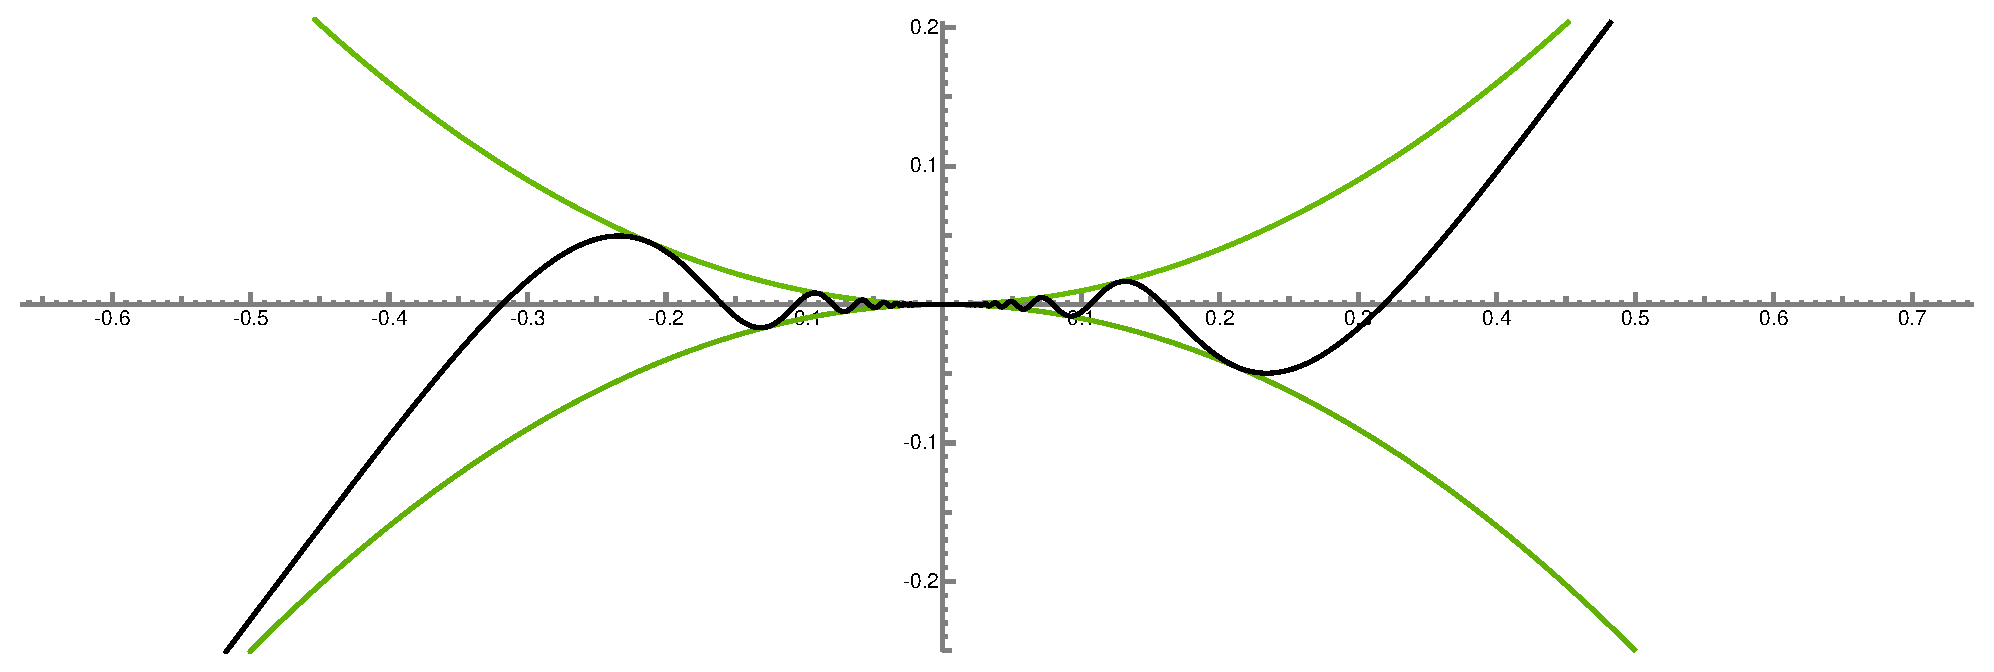
\includegraphics[height=4cm]{darboux.pdf}
  \centering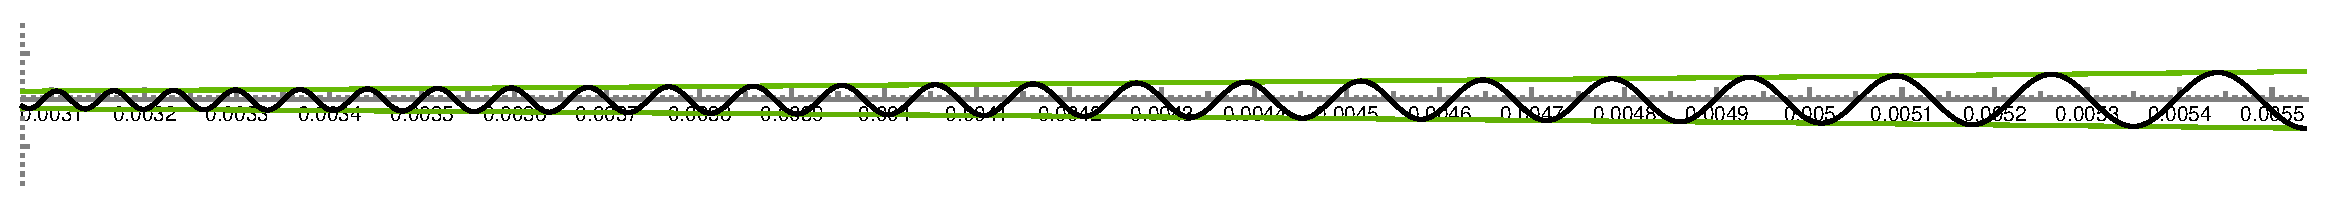
\includegraphics[width=\textwidth]{darboux2.pdf}
  \begin{comment}
  \begin{tikzpicture}[scale=5]
    \draw[->] (-0.5, 0) -- (0.5, 0) node[above] {$x$};
    \draw[->] (0, -0.3) -- (0, 0.3) node[right] {$y$};
    \draw[domain=-0.51:0.5, smooth, variable=\x, gray] plot ({\x}, {\x*\x});
    \draw[domain=-0.51:0.5, smooth, variable=\x, gray] plot ({\x}, {-\x*\x});
    \draw[domain=-0.51:0.5, variable=\x, samples=200, blue, thick] plot ({\x}, {\x*\x*sin(deg(1/\x))});
  \end{tikzpicture}
  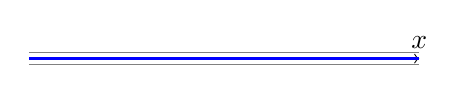
\begin{tikzpicture}[scale=5000]
    \draw[->] (0.0045, 0) -- (0.0055, 0) node[above] {$x$};
    \draw[domain=0.0045:0.0055, smooth, variable=\x, gray] plot ({\x}, {\x*\x});
    \draw[domain=0.0045:0.0055, smooth, variable=\x, gray] plot ({\x}, {-\x*\x});
    \draw[domain=0.0045:0.0055, variable=\x, samples=200, blue, thick] plot ({\x}, {\x*\x*sin(deg(1/\x))});
  \end{tikzpicture}
  \end{comment}
  \caption{Il grafico di una funzione derivabile ma con 
    derivata non continua (vedi esempio~\ref{ex:derivata_non_continua}).
    L'ingrandimento nel disegno in basso rende evidente 
    il fatto che la derivata oscilla tra i valori 
    $-1$ e $1$ in ogni intorno di $0$.
    La proprietà di Darboux (teorema~\ref{th:darboux})
    rimane comunque soddisfatta: la derivata assume tutti i valori 
    compresi tra $1$ e $-1$ in ogni intorno di $x=0$ ma 
    non ha limite per $x\to 0$.\\\\
    \usebox{\qrdarboux}
}
\end{figure}

\begin{example}
[funzione derivabile con derivata non continua]
\label{ex:derivata_non_continua}%
\mymark{**}%
\index{funzione!derivabile con derivata non continua}%
\index{derivata!non continua}%
La funzione $f\colon \RR \to \RR$ definita da
\[
  f(x)
  = \begin{cases}
    x^2 \sin(1/x) & \text{se $x \neq 0$} \\
    0 & \text{se $x=0$.}
  \end{cases}
\]
è derivabile su tutto $\RR$, $f'(0)=0$ ma il limite
\[
\lim_{x\to 0} f'(x)
\]
non esiste (e dunque $f'\colon \RR\to\RR$ non è continua in $x=0$).
\end{example}
%
\begin{proof}
La funzione $x^2 \sin(1/x)$ è derivabile infinite volte su tutto il suo dominio $\RR\setminus\ENCLOSE{0}$ in quanto composizione di funzioni elementari derivabili infinite volte.
Dunque, per la località della derivata, anche la funzione $f$ è derivabile infinite volte su $\RR\setminus\ENCLOSE{0}$.
Per $x\neq 0$ possiamo quindi calcolare $f'(x)$ utilizzando le regole di derivazione
\[
  f'(x)
  = D \enclose{x^2\sin \frac 1 x}
  = 2x \sin \frac 1 x + x^2 \enclose{\cos \frac 1 x} \cdot\frac{-1}{x^2}
  = 2x \sin \frac 1 x - \cos \frac 1 x.
\]

Verifichiamo ora che $f$ è continua e derivabile anche in $0$.
Si ha infatti
\[
 \lim_{h\to 0}\frac{f(0+h)-f(0)}{h}
 = \lim_{h\to 0} h \sin \frac 1 h = 0
\]
e dunque $f'(0) = 0$.
Osserviamo però che $f'(x)$ non ammette limite per $x\to 0$
in quanto per $x \to 0$ si ha $2x \sin(1/x) \to 0$ ma il limite di $\cos (1/x)$ invece non esiste. Dunque $f'(x)$ è la somma di una funzione che ha limite zero e di una funzione il cui limite non esiste per $x\to 0$. Dunque $f'(x)$ non ammette limite per $x\to 0$.
\end{proof}

\begin{proposition}[criterio di derivabilità]%
\label{prop:4384774}\mymark{**}%
Sia $I\subset \RR$ un intervallo, $x_0\in I$,
$f\colon I \to \RR$ una funzione continua su tutto $I$ 
e derivabile in $I\setminus\ENCLOSE{x_0}$.
Se il limite della derivata
\[
  \lim_{x\to x_0} f'(x) = m
\]
esiste ed è finito la funzione $f$ è derivabile anche in $x_0$ e vale $f'(x_0) = m$.
\end{proposition}
%
\begin{proof}
\mymark{*}
Prendiamo un generico punto $x>x_0$ (il caso $x<x_0$ è del tutto analogo).
Per il teorema
di Lagrange sappiamo esistere un punto $y\in (x_0,x)$ tale che
\[
  \frac{f(x)-f(x_0)}{x-x_0} = f'(y).
\]
Per $x\to x_0$ si ha certamente anche $y\to x_0$ e dunque
esiste il limite del rapporto incrementale:
\[
  f'(x_0) = \lim_{x\to x_0} \frac{f(x)-f(x_0)}{x-x_0}
  = \lim_{y\to x_0} f'(y) = m.
\]
\end{proof}
%
La proposizione precedente dice che la derivata di una funzione in un
punto non può avere un valore diverso dal suo limite, se tale limite esiste.
Esistono però funzioni derivabili la cui derivata non è
continua, come abbiamo visto
nell'esempio~\ref{ex:derivata_non_continua}
in quanto il limite della derivata potrebbe non esistere.


\section{convessità}

\begin{definition}[funzione convessa]
\mymark{**}
Sia $I\subset \RR$ un intervallo.
Una funzione $f\colon I\to \RR$
si dice essere
\emph{convessa}
\mymargin{funzione convessa}
\index{funzione!convessa}
se per ogni $x,y\in I$ e per ogni $t\in [0,1]$ si ha
\[
f((1-t)x + ty) \le (1-t) f(x) + t f(y).
\]

Analogamente diremo che $f$ è \emph{concava} 
\mymargin{funzione concava}%
\index{funzione!concava}%
se vale la disuguaglianza inversa:
\[
f((1-t)x + ty) \ge (1-t) f(x) + t f(y)
\]
(o, equivalentemente, se $-f$ è convessa).
\end{definition}

Osserviamo che la retta del piano passante per i punti $(x,f(x))$ e $(y,f(y))$ può essere parametrizzata in maniera uniforme per $t\in \RR$
da
\[
  (1-t) (x,f(x)) + t(y,f(y)) = ((1-t)x + ty, (1-t) f(x) + tf(y)).
\]
Chiaramente per $t=0$ si ottiene il punto $(x,f(x))$ per $t=1$ il punto $(y,f(y))$ e per $t\in[0,1]$ il segmento congiungente tali punti. La condizione di convessità della funzione $f$ corrisponde quindi a richiedere che ogni corda (segmento) che unisce due punti del grafico si trovi "al di sopra" del grafico della funzione.

\begin{definition}[insieme convesso]
\mymark{*}
Un insieme $E\subset \RR^n$ si dice essere \emph{convesso}%
\mymargin{convesso}%
\index{convesso} se dati
due punti qualunque $a,b\in E$ l'intero segmento $[a,b]=\ENCLOSE{(1-t)a+tb\colon t\in [0,1]}$ è contenuto in $E$.
\end{definition}

\begin{theorem}[epigrafico delle funzioni convesse]
Sia $I\subset \RR$ e $f\colon I\subset \RR\to \RR$ una funzione.
Allora sono equivalenti:
\begin{enumerate}
\item $I$ è un intervallo e $f$ è convessa;
\item l'\emph{epigrafico di $f$}%
\mymargin{epigrafico di $f$}%
\index{epigrafico} (o \emph{sopragrafico})
\index{epigrafico}
ovvero l'insieme
\[
  E = \ENCLOSE{(x,y)\in \RR^2\colon x\in I, y\ge f(x)}
\]
è convesso.
\end{enumerate}

Per le funzioni concave sarà il \emph{sottografico} $\ENCLOSE{(x,y)\colon y\le f(x)}$ ad essere convesso.
\end{theorem}
%
\begin{proof}
Supponiamo che $I$ sia un intervallo e $f$ sia convessa. Per dimostrare che l'epigrafico $E$ è convesso consideriamo due punti $a,b\in E$ e un qualunque punto $p$ sul segmento $[a,b]$.
Se $a=(x_a, y_a)$, $b=(x_b,y_b)$, $p=(x_p, y_p)$
allora esiste un $t\in [0,1]$ tale che $x_p = (1-t)x_a + t x_b$ e $y_p=(1-t)y_a + t y_b$.
Visto che $a,b\in E$ sappiamo che $y_a \ge f(x_a)$ e $y_b\ge f(x_b)$. Dunque necessariamente si ha
\[
  y_p \ge (1-t)f(x_a) + t f(y_b).
\]
Ma essendo $f$ convessa si ha:
\[
  (1-t)f(x_a) + t f(y_b) \ge f((1-t)x_a + t x_b) = f(x_p).
\]
Dunque $y_p\ge f(x_p)$ che significa $p\in E$.

Viceversa supponiamo di sapere che $E$ è convesso. Siano $x,y\in I$ punti qualunque. Allora i punti $a=(x,f(x))$ e $b=(y,f(y))$ sono certamente punti di $E$ e quindi l'intero segmento $[a,b]$ deve essere contenuto in $E$. Dunque per ogni $t\in [0,1]$ il punto $p = ((1-t)x + t y,$ $(1-t)f(x)+ tf(y))$ deve stare in $E$. In primo luogo deve quindi essere $(1-t)x+ty\in I$ e se questo è vero per ogni $t\in[0,1]$ significa che $I$ è un intervallo. In secondo luogo se $p\in E$ significa che
\[
  (1-t)f(x) +t f(y) \ge f((1-t)x + t y)
\]
che corrisponde alla definizione di funzione convessa.
\end{proof}


\begin{lemma}[rapporto incrementale di una funzione convessa]
\mymark{*}%
\label{lemma:547091}%
Sia $I$ un intervallo di $\RR$ e sia $f\colon I\to \RR$.
Dati $x,y\in I$ con $x\neq y$ definiamo il \emph{rapporto incrementale}
di $f$ come:
\[
  R(x,y) = \frac{f(y) - f(x)}{y-x}.
\]
Allora sono condizioni equivalenti:
\begin{enumerate}
\item $f$ è convessa;
\item per ogni $x,y,z\in I$ se $x<y<z$ si ha $R(x,y)\le R(y,z)$;
\item per ogni $x,y,z\in I$ se $x<y<z$ si ha $R(x,y)\le R(x,z)$;
\item per ogni $x,y,z\in I$ se $x<y<z$ si ha $R(x,z)\le R(y,z)$;
\item la funzione $R(x,y)$ è crescente in ognuna delle due variabili.
\end{enumerate}
\end{lemma}
%
\begin{proof}
Attenzione:
il lemma risulta ovvio se si utilizza la giusta interpretazione geometrica
(il rapporto incrementale è la pendenza della corda corrispondente).
Quella che segue è la traduzione algebrica di quanto
è geometricamente ovvio ma risulta inevitabilmente pesante
e più difficilmente comprensibile.

Siano $x,y,z\in I$ con $x<y<z$.
Posto $t=(y-x)/(z-x)$ si ha $y=(1-t)x + tz$,
 $y-x = t(z-x)$, $z-y = (1-t)(z-x)$.
Si ha allora
 \begin{equation*}
 \begin{aligned}
 R(x,z) - R(x,y)
 &= \frac{f(z)-f(x)}{z-x} - \frac{f(y)-f(x)}{y-x} \\
  &= t\frac{f(z)-f(x)}{y-x} - \frac{f(y)-f(x)}{y-x} \\
  &= \frac{tf(z) + (1-t) f(x) - f(y)}{y-x}
 \end{aligned}
 \end{equation*}

La condizione di convessità di $f$ è
\[
  f(y) \le (1-t)f(x) + tf(z)
\]
ed è quindi equivalente alla condizione $R(x,y) \le R(x,z)$.
Dunque le condizioni 1 e 3 sono equivalenti.

Ma con una verifica diretta si osserva che
\[
  R(x,z) = t R(x,y) + (1-t) R(y,z)
\]
da cui si ottiene
\[
  R(y,z) - R(x,z) = t[R(y,z) - R(x,y)]
\]
oppure anche
\[
 R(x,z) - R(x,y) = (1-t) [R(y,z) - R(x,y)].
\]
Risulta quindi che le quantità
\[
  R(y,z) - R(x,y), \qquad
  R(x,z) - R(x,y), \qquad
  R(y,z) - R(x,z)
\]
hanno tutte lo stesso segno. E quindi le condizioni 2, 3 e 4 sono tra loro equivalenti (se vale una delle tre valgono tutte e tre).

Se valgono le tre condizioni 2, 3 e 4 è facile verificare che la funzione $R(x,y)$ è crescente in entrambe le variabili. Innanzitutto per simmetria, visto che $R(x,y) = R(y,x)$, è sufficiente verificare che $R(x,y)$ è crescente nella seconda variabile $y$ per ogni $x$ fissato. Quindi dato $z>y$ bisogna mostrare che $R(x,z) \ge R(x,y)$.
Abbiamo allora tre possibilità a seconda che sia $x<y$ oppure $y<x<z$ oppure $z<x$. Nel primo caso si ha $x<y<z$ e dunque la disuguaglianza $R(x,y) \le R(x,z)$ corrisponde alla condizione 3.
Nel secondo caso si ha $y<x<z$ e la condizione $R(x,y)\le R(x,z)$ si può scrivere come $R(y,x) \le R(x,z)$ che è, riordinando opportunamente le variabili, la condizione 2. Se, infine, $y < z < x$ la condizione $R(x,y) \le R(x,z)$ si può scrivere $R(y,x) \le R(z,x)$ che, riordinando le variabili, è la condizione 4.

Viceversa (e infine) se la funzione $R(x,y)$ è crescente in entrambe le variabili in particolare è crescente nella seconda variabile e quindi se $x<y<z$ si ha $R(x,y) \le R(x,z)$. Risulta quindi che la condizione 5 implica la 3 e quindi tutte le altre condizioni.
\end{proof}

\begin{theorem}
\mymark{***}
Sia $I\subset \RR$ un intervallo e $f\colon I \to \RR$ una funzione derivabile su tutto $I$.
Allora sono equivalenti:
\begin{enumerate}
\item $f$ è convessa;
\item per ogni $x_0 \in I$ e per ogni $x\in I$ si ha
\[
   f(x) \ge f'(x_0) (x-x_0) + f(x_0)
\]
(geometricamente: il grafico della funzione sta sopra la retta tangente);
\item $f'$ è crescente.
\end{enumerate}

Analogamente per le funzioni concave si avrà che il grafico ``sta sotto'' la retta tangente e che la derivata è decrescente.
\end{theorem}
%
\begin{proof}
\mymark{**}
Osserviamo che
\[
  f'(x_0) = \lim_{x\to x_0} R(x_0,x).
\]
Se $f$ è convessa allora, per il lemma, il rapporto incrementale $R(x_0,x)$ è crescente e quindi  $f'(x_0) = \inf_{x>x_0} R(x_0,x)$. In particolare $f'(x_0) \le R(x_0,x)$ per ogni $x> x_0$. In maniera analoga si trova $f'(x_0) \ge R(x_0,x)$ se $x<x_0$.
In ogni caso risulta quindi che per ogni $x$ si ha
\[
(R(x_0,x)- f'(x_0))(x-x_0)\ge 0
\]
ovvero
\[
  f(x) - f(x_0) - f'(x_0)(x-x_0) \ge 0.
\]
Dunque la condizione 1 implica la 2.

Se vale la condizione 2, dati $x,y \in I$ si ha
\[
  f(x) - f(y) \ge f'(y)(x-y)
\]
se scambiamo $x$ e $y$ e cambiamo di segno ambo i membri si ottiene invece
\[
  f(x) - f(y) \le f'(x)(x-y)
\]
mettendo insieme le due disuguaglianze,
se ora supponiamo che sia $x>y$ otteniamo proprio
$f'(x) \ge f'(y)$ cioè $f'$ è crescente (condizione 3).

Supponiamo ora di sapere che $f'$ è crescente e supponiamo per assurdo che la funzione $f$ non sia convessa.
In base al lemma precedente dovrebbero allora esistere tre punti $x<y<z$ tali che $R(x,y)> R(y,z)$. Per il teorema di Lagrange dovrebbe allora esistere un punto $c\in (x,y)$ tale che $f'(c) = R(x,y)$ e un punto $d \in (y,z)$ tale che $f'(d) = R(y,z)$ ma allora
$f'(c) > f'(d)$ nonostante sia $c<d$ e dunque $f'$ non poteva essere crescente.
\end{proof}

\begin{corollary}[criterio di convessità tramite derivata seconda]
\mymark{***}
Sia $I\subset \RR$ un intervallo e sia $f\colon I \to \RR$ una funzione derivabile due volte (cioè $f$ è derivabile e anche $f'$ è derivabile).
Allora $f$ è convessa se e solo se $f''(x)\ge 0$ per ogni $x\in I$.
Analogamente $f$ è concava se e solo se $f''\le 0$.
\end{corollary}
\begin{proof}
\mymark{***}
Per il criterio precedente $f$ è convessa se e solo se $f'$ è crescente. Per il criterio di monotonia $f'$ è crescente se e solo se $f'' \ge 0$. Considerazioni analoghe valgono per la concavità.
\end{proof}

\begin{theorem}
Siano $a\in \RR$, $b\in \bar \RR$, $a<b$.
Sia $f\colon [a,b)\to \RR$ una funzione convessa in $(a,b)$ e continua in $a$. Allora $f$ è convessa su tutto $[a,b)$. Risultato analogo vale per funzioni definite su intervalli aperti a sinistra $(a,b]$
e aperti da ambo i lati $(a,b)$.
\end{theorem}
%
\begin{proof}
Dati $x,y \in [a,b)$ dobbiamo mostrare che per ogni $t\in[0,1]$ vale
\[
f((1-t) x+ t y) \le (1-t)f(x) + t f(y).
\]
Per ipotesi sappiamo che la disuguaglianza è valida se $x,y \in (a,b)$. Dobbiamo quindi dimostrare la disuguaglianza solamente nel caso $x=a$ e $y\in(a,b)$. Dato qualunque $t\in (0,1)$ e
presa una successione $x_k \to a$ con $x_k\in (a,b)$ definiamo
$t_k$ in modo che sia $z = (1-t)x + ty = (1-t_k) x_k + t_k y$
cioè:
\[
  t_k = \frac{x - x_k + t(y-x)}{y-x_k}.
\]
Siccome $t_k\to t$ per $k\to +\infty$ se $t\in (0,1)$ per $k$ abbastanza grande anche $t_k\in(0,1)$. Inoltre per la convessità in $(a,b)$ sappiamo che vale
\[
  f((1-t_k)x_k + t_k y) \le (1-t_k) f(x_k) + t_k f(y)
\]
e passando a limite per $k\to +\infty$, dalla continuità di $f$ in $x$ si ottiene
\[
   f((1-t)x+ty) \le (1-t) f(x) + t f(y)
\]
come volevamo dimostrare. Per $t=0$ e $t=1$ la disuguaglianza è sempre banalmente verificata.
\end{proof}

\begin{example}
La funzione $f(x) = \sqrt{x}$ è definita su $[0,+\infty)$ ma è derivabile solamente in $(0,+\infty)$. La sua derivata è $f'(x) = x^{-\frac 1 2 }/2$ e la derivata seconda è $f''(x) = -x^{-\frac 3 2}/4 < 0$. Dunque la funzione è concava sull'intervallo aperto $(0,+\infty)$. Ma essendo continua possiamo concludere che $f$ è concava su tutto il dominio $[0,+\infty)$.
\end{example}

\begin{comment}
\begin{theorem}[continuità delle funzioni convesse]
Siano $a,b \in \bar \RR$ con $a< b$.
Sia $f\colon (a,b) \to \RR$ una funzione convessa. Allora $f$ è continua.
\end{theorem}
%
\begin{proof}
Sia $x_0 \in (a,b)$ e siano $y,z \in (a,b)$ con $y < x_0 < z$.
Per il lemma sui rapporti incrementali sappiamo che per ogni $x\in (y,z)$ si ha
\[
   R(x_0, y) \le R(x_0,x) \le R(x_0,z).
\]
In particolare esiste una costante $C$ tale che
\[
  \abs{R(x_0,x)} \le C,\qquad \forall x \in (y,z).
\]
Moltiplicando per $\abs{x-x_0}$ si ottiene allora
\[
   \abs{f(x) - f(x_0)} \le C \abs{x-x_0}
\]
e per $x\to x_0$ il lato destro tende a zero e quindi per confronto anche il lato sinistro deve tendere a zero. Dunque $f(x)\to f(x_0)$
e $f$ è continua in $x_0$.
\end{proof}
\end{comment}

\begin{theorem}[derivabilità delle funzioni convesse]
  Sia $I\subset \RR$ un intervallo e sia $f\colon I \to \RR$ una funzione convessa.
  Se $x_0\in (\inf I, \sup I)$ esistono e sono finite la derivata destra 
  e sinistra di $f$ in $x_0$:
  \begin{align*}
    f'_+(x_0) &= \lim_{x\to x_0^+} \frac{f(x)-f(x_0)}{x-x_0}\\
    f'_-(x_0)  &= \lim_{x\to x_0^-} \frac{f(x)-f(x_0)}{x-x_0}  
  \end{align*}
  e risulta
  \[
    f'_-(x_0) \le f'_+(x_0).
  \]
  Inoltre se $\inf I < x_1 < x_2 < \sup I$ si ha 
  \[
    f'_+(x_1) \le f'_(x_2).
  \]
  Se ne deduce che $f$ è continua in tutti i punti interni di $I$ 
  e che l'insieme dei punti in cui $f$ non è derivabile 
  è al più numerabile.
  \end{theorem}
  %
  \begin{proof}
    Nel lemma~\ref{lemma:547091} abbiamo osservato che il rapporto incrementale
    \[
      R(x_0,x) = \frac{f(x)-f(x_0)}{x-x_0}
    \] 
    di una funzione convessa è crescente rispetto alla variabile $x$. 
    Dunque per il teorema~\ref{th:limite_monotona} si 
    ha 
    \[
      f'_-(x_0) = \sup_{x<x_0} R(x_0,x)>-\infty, \qquad 
      f'_+(x_0) = \inf_{x>x_0} R(x_0,x)<+\infty
    \]
    e visto che se $x<x_0$ e $y>x_0$ si ha $R(x_0,x)\le R(x_0,y)$ 
    deduciamo che $f'_-(x_0)\le f'_+(x_0)$ ed entrambi i limiti 
    sono dunque finiti. Se $x_1 < x_2$ allora preso un qualunque 
    punto $x$ con $x_1<x<x_2$ si ha (sempre per il lemma~\ref{lemma:547091})
    \[
      R(x_1,x) \le R(x,x_2)
    \]
    e dunque passando al limite si trova $f'_+(x_1) \le f'_-(x_2)$.
    Le derivate destra e sinistra esistono dunque in tutti i punti interni 
    all'intervallo $I$. 
    In particolare $f$ è continua in tali punti in quanto è continua sia da destra 
    che da sinistra.
    I punti di non derivabilità di $f$ sono i punti in cui 
    le derivate destra e sinistra differiscono. 
    Ma ad ogni punto $x$ di non differenziabilità 
    posso associare l'intervallo aperto non vuoto $I_x = (f'_-(x),f'_+(x))$ e per 
    le proprietà appena viste è chiaro che questi intervalli sono a due a due disgiunti
    in quanto se $x_1<x_2$ l'estremo destro di $I_{x_1}$ è minore o uguale all'estremo 
    sinistro di $I_{x_2}$.
    Siccome ognuno di questi intervalli contiene almeno un numero razionale concludiamo che 
    il numero di punti di discontinuità non può essere maggiore della cardinalità 
    dei numeri razionali.
  \end{proof}
  
  \begin{theorem}[retta di supporto]
    \label{th:supporto_convessa}%
    Sia $I\subset \RR$ un intervallo, $f\colon I\to\RR$ una funzione convessa 
    e $x_0$ un punto interno ad $I$. Allora esiste una funzione lineare affine 
    \[
      L(x) = mx+q
    \]
    tale che $f(x_0) = L(x_0)$ e per ogni $x\in I$ si abbia $f(x)\ge L(x)$.
  \end{theorem}
  %
  \begin{proof}
    Basta scegliere qualunque $m\in [f'_-(x_0),f'_+(x_0)]$ e considerare la funzione 
    lineare affine $L(x) = m(x-x_0)$. Se $x>x_0$ allora si ha $R(x_0,x)\ge m$ 
    e dunque $f(x) - f(x_0) \ge m (x-x_0) = L(x)$. Viceversa se $x<x_0$ 
    si ha $R(x_0,x)\le m$ da cui, di nuovo, $f(x)-f(x_0) \ge m(x-x_0) = L(x)$.
  \end{proof}
  %
  Il seguente teorema può essere enunciato anche per gli integrali 
  come vedremo nel teorema~\ref{th:jensen}. 
  La dimostrazione è sostanzialmente identica ed è valida anche 
  per funzioni convesse di più variabili.
  %
  \begin{theorem}[combinazioni baricentriche/disuguaglianza di Jensen]
    \mymark{*}%
    \label{th:combinazioni_baricentriche}%
    \index{combinazioni baricentriche}%
    \index{disuguaglianza!di Jensen}%
    \index{Jensen!disuguaglianza di}%
    Se $f$ è una funzione convessa definita su un intervallo $I$, dati $x_1, \dots, x_n \in I$ e $\lambda_1, \dots, \lambda_n\in \RR$ tali che $\sum_{k=1}^n \lambda_k = 1$ e $\lambda_k \ge 0$ per ogni $k=1, \dots, n$ allora
    \[
      f\enclose{\sum_{k=1}^n \lambda_k x_k}
      \le \sum_{k=1}^n \lambda_k f(x_k).
    \]
    Per le funzioni concave vale la disuguaglianza inversa.
    \end{theorem}
    %
    \begin{comment}
    \begin{proof}
    Procediamo per induzione su $n$. Nel caso $n=1$ si ha $\lambda_1=1$ e i due lati della disuguaglianza sono effettivamente uguali. Supponendo il teorema dimostrato per un certo $n$, procediamo a dimostrarlo per $n+1$.
    Osserviamo che
    \begin{align*}
      \sum_{k=1}^{n+1} \lambda_k x_k
      &= \sum_{k=1}^n \lambda_k x_k  + \lambda_{n+1} x_{n+1} \\
      &= (1-\lambda_{n+1})\sum_{k=1}^n\frac{\lambda_k}{1-\lambda_{n+1}} x_k + \lambda_{n+1} x_{n+1}.
    \end{align*}
    Visto che
    \[
      \sum_{k=1}^{n+1} \lambda_k = 1
    \]
    si ha
    \[
      \sum_{k=1}^n \frac{\lambda_k}{1-\lambda_{n+1}}
      = \frac{1-\lambda_{n+1}}{1-\lambda_{n+1}} = 1.
    \]
    Dunque, per ipotesi induttiva si ha allora
    \[
      f\enclose{\sum_{k=1}^n\frac{\lambda_k}{1-\lambda_{n+1}} x_k}
      \le \sum_{k=1}^n \frac{\lambda_k}{1-\lambda_{n+1}}f(x_k).
    \]
    Usando di nuovo la convessità di $f$ con $t=\lambda_{n+1}$ si ha
    \begin{align*}
    f\enclose{\sum_{k=1}^{n+1} \lambda_k x_k}
    &=f\enclose{(1-\lambda_{n+1})\sum_{k=1}^n \frac{\lambda_k}{1-\lambda_{n+1}}x_k + \lambda_{n+1}x_{n+1}}\\
    &\le (1-\lambda_{n+1})f\enclose{\sum_{k=1}^n \frac{\lambda_k}{1-\lambda_{n+1}}x_k} + \lambda_{n+1}f(x_{n+1}) \\
    &\le (1-\lambda_{n+1})\sum_{k=1}^n \frac{\lambda_k}{1-\lambda_{n+1}} f(x_k) + \lambda_{n+1} f(x_{n+1})\\
    &= \sum_{k=1}^{n+1}\lambda_k f(x_k).
    \end{align*}
    come volevamo dimostrare.
    \end{proof}
  \end{comment}
  %    
  \begin{proof}
  Poniamo 
  \[
    \bar x =  \sum_{k=1}^n \lambda_k x_k.
  \]
  Per il teorema~\ref{th:supporto_convessa} precedente 
  sappiamo che esiste una retta $L(x) = mx + q$ 
  tale che $L(\bar x) = f(\bar x)$ 
  e $L(x)\le f(x)$ per ogni $x \in I$.
  Allora si ha 
  \[
  L \enclose{\sum_{k=1}^n \lambda_k x_k}
  = \sum_{k=1}^n m \lambda_k x_k + q \sum_{k=1}^n \lambda_k 
  = \sum_{k=1}^n \lambda_k L(x_k).  
  \]
  Dunque 
  \[
  f(\bar x) = L(\bar x) = \sum_{k=1}^n \lambda_k L(x_k) \le 
  \sum_{k=1}^n \lambda_k f(x_k).
  \]
  \end{proof}

\begin{example}[disuguaglianza tra media aritmetica e media geometrica]
\mymark{*}
\index{disuguaglianza!media aritmetica media geometrica}
Osserviamo che la funzione $f(x) = \ln x$ è concava, infatti si ha
$f''(x) = -1/x^2 < 0$. Dunque, per il teorema precedente, se $\lambda_1 + \dots + \lambda_n =1$, $\lambda_k \ge 0$ si ha
\[
    \ln\enclose{\sum_{k=1}^n \lambda_k x_k}
    \ge \sum_{k=1}^n \lambda_k \ln x_k.
\]
Facendo l'esponenziale di ambo i membri si ottiene
\[
  \sum_{k=1}^n \lambda_k x_k \ge \prod_{k=1}^n x_k^{\lambda_k}.
\]
Nel caso particolare $\lambda_k = 1/n$ si ottiene
la disuguaglianza tra \emph{media aritmetica} (AM per gli anglofoni)
e \emph{media geometrica}
\mymargin{media aritmetica geometrica}%
\index{media aritmetica geometrica}%
\index{media!aritmetica}%
\index{media!geometrica}%
\index{AM}%
\index{GM}%
(GM):
\[
  \frac{x_1 + \dots + x_n}{n} \ge \sqrt[n]{x_1\cdots x_n}.
\]
\end{example}

\begin{exercise}[subadditività delle funzioni concave]
Sia $f\colon [0,+\infty) \to \RR$ una funzione concava con $f(0)\ge 0$. Allora $f$ è subadditiva cioè:
\[
  f(x+y) \le f(x) + f(y),\qquad \forall x,y\ge 0.
\]
\end{exercise}
%
\begin{proof}
Se $x=y=0$ la disuguaglianza è ovvia.
Altrimenti $x+y>0$ e si ha
\begin{align*}
f(x) &= f\enclose{\frac{y}{x+y}\cdot 0 + \frac{x}{x+y}\cdot (x+y)}\\ &\ge \frac{y}{x+y}f(0) + \frac{x}{x+y}f(x+y)
\ge \frac{x}{x+y}f(x+y).
\end{align*}
Scambiando $x$ con $y$ e sommando si ottiene:
\[
  f(x) + f(y) \ge \frac{x}{x+y}f(x+y) + \frac{y}{x+y}f(x+y) = f(x+y).
\]
\end{proof}

Si osservi che sviluppando la disuguaglianza $(x-y)^2\ge 0$ si ottiene:
\[
  x y \le \frac{x^2 + y^2}{2}.
\]
Questa disuguaglianza può essere generalizzata ad esponenti diversi 
come si vede nel seguente.

\begin{theorem}[disuguaglianza di Young]%
\label{th:young}%
\index{Young!disuguaglianza di}%
\index{disuguaglianza!di Young}%
Se $p>1$, $q>1$, $\frac{1}{p}+\frac{1}{q}=1$, $x,y\ge 0$:
\begin{equation}\label{eq:young}
  x y \le \frac{x^p}{p} + \frac{y^q}{q}.
\end{equation}
\end{theorem}
%
\begin{proof}
Si utilizza la disuguaglianza di convessità per la funzione $\exp(x)=e^x$. 
Visto che la derivata seconda dell'esponenziale è positiva, la funzione $\exp$ 
è convessa e dunque, se $x>0$ e $y>0$ si ha:
\begin{align*}
 x\cdot y 
  &= \exp(\ln x + \ln y)
  = \exp\enclose{\frac 1 p \ln (x^p) + \frac 1 q \ln (y^q)}  \\
  &\le \frac 1 p \cdot \exp \ln (x^p) + \frac 1 q \exp \ln (y^q)
  = \frac{x^p}{p} + \frac{y^q}{q}.
\end{align*}
Se $x=0$ o $y=0$ la disuguaglianza è ovvia in quanto il lato sinistro 
di~\eqref{eq:young} è nullo.
\end{proof}

\begin{theorem}[disuguaglianza di Hölder]
Se $a_k\ge 0$ e $b_k\ge 0$ per $k\in \NN$
e siano $p>1$ e $q>1$ tali che $\frac 1 p + \frac 1 q = 1$.
Allora 
\[
 \sum_k a_k b_k  \le \enclose{\sum_k a_k^p}^{1 \over p} \cdot \enclose{\sum_k b_k^q}^{1\over q}.
\]
\end{theorem}
\begin{proof}
Poniamo 
\[
A = \enclose{\sum_k a_k^p}^{1 \over p}, \qquad 
B = \enclose{\sum_k b_k^q}^{1\over q}.
\]
Se $A>0$ e $B>0$ possiamo dividere il lato sinistro della disuguaglianza 
per il lato destro e applicare la disuguaglianza~\eqref{eq:young} di Young:
\begin{align*}
  \frac{\sum_k a_k b_k}{A\cdot B} 
  & = \sum_k \frac{a_k}{A}\cdot \frac{b_k}{B} 
  \le \sum_k \frac 1 p \frac{a_k^p}{A^p} + \frac 1 q \frac{b_k^q}{B^q} \\
  &= \frac 1 p \frac{\sum_k a_k^p}{A^p} + \frac 1 q \frac{\sum_k b_k^q}{B^q}
  = \frac 1 p + \frac 1 q = 1.
\end{align*}
E il teorema e dimostrato. 

Se fosse $A=0$ tutti i termini $a_k$ sarebbero nulli e la disuguaglianza 
si riduce banalmente a $0\le 0$. Lo stesso se fosse $B=0$.  
\end{proof}

Nel caso $p=q=2$ si ottiene la 
\emph{disuguaglianza di Cauchy-Schwarz}%
\mymargin{disuguaglianza di Cauchy-Schwarz}%
\index{disuguaglianza!di Cauchy-Schwarz}
\index{disuguaglianza!di Cauchy-Schwarz}%
\index{Cauchy-Schwarz!disuguaglianza di}%
\index{Schwarz!disuguaglianza di Cauchy-}%
\[
   \sum_k \abs{a_k b_k} \le \sqrt{\sum_k a_k^2} \cdot \sqrt{\sum_k b_k^2}
\]
che potrebbe però essere più facilmente dimostrata 
per un generico prodotto scalare, come faremo 
nel teorema~\ref{th:spazio_euclideo}.

\section{teoremi di Cauchy e de l'Hospital}

\begin{theorem}[Cauchy]
\label{th:cauchy}%
\mymark{**}%
\index{teorema!di Cauchy}%
\mymargin{Cauchy}%
\index{Cauchy}%
Siano $a,b\in \RR$, $a < b$.
\mynote{Se $b<a$ il teorema è ugualmente valido intendendo $[a,b]=[b,a]$.}%
Siano $f\colon[a,b]\to \RR$ e $g\colon[a,b]\to \RR$ funzioni continue su tutto $[a,b]$ e derivabili su $(a,b)$.
Supponiamo inoltre che $g'(x)\neq 0$ per ogni $x\in (a,b)$.
Allora $g(b) \neq g(a)$ ed esiste $x_0\in(a,b)$ tale che
\[
  \frac{f'(x_0)}{g'(x_0)} = \frac{f(b)-f(a)}{g(b)-g(a)}.
\]
\end{theorem}
%
\begin{proof}
\mymark{**}
Si consideri la funzione ausiliaria
\[
 h(x) = (g(b)-g(a))f(x) - (f(b)-f(a))g(x).
\]
Per verifica diretta si osserva che
\[
  h(b) = g(b)f(a) - f(b)g(a) = h(a).
\]
Dunque $h$ verifica le ipotesi del teorema di Rolle ed esiste
dunque un punto $x_0\in(a,b)$ per cui $h'(x_0) = 0$.
Essendo però
\[
  h'(x) = (g(b) - g(a)) f'(x) - (f(b)-f(a)) g'(x)
\]
si ottiene
\[
 (g(b)-g(a))f'(x_0) = (f(b) - f(a))g'(x_0).
\]
Per ipotesi sappiamo che $g'(x_0)\neq 0$.
Ma necessariamente anche $g(b) - g(a)\neq 0$ perché altrimenti potremmo applicare il teorema di Rolle alla funzione $g$ e ottenere che $g'$ si annulla in un punto di $(a,b)$, cosa che abbiamo escluso per ipotesi.
Dunque possiamo dividere ambo i membri per $(g(b)-g(a))$ e per $g'(x_0)$ per ottenere l'uguaglianza enunciata nel teorema.
\end{proof}

\begin{theorem}[de l'Hospital $0/0$]
\mymark{***}
Sia $I\subset \RR$ un intervallo, $x_0\in [-\infty,+\infty]$ un punto di accumulazione
di $I$
e siano $f,g \colon I\setminus\ENCLOSE{x_0} \to \RR$ funzioni derivabili.
Supponiamo che sia $g'(x)\neq 0$ per ogni $x\in I\setminus\ENCLOSE{x_0}$.
Se
\[
  \lim_{x\to x_0} f(x) = 0 \qquad \text{e}\qquad \lim_{x\to x_0} g(x) = 0
\]
e se esiste (finito o infinito) il limite
\[
  \ell = \lim_{x\to x_0}\frac{f'(x)}{g'(x)}
\]
allora si ha
\[
  \lim_{x\to x_0} \frac{f(x)}{g(x)} = \ell.
\]
\end{theorem}
%
\begin{proof}
\mymark{**}
Bisognerà distinguere diversi casi a seconda che $x_0$ sia finito o infinito
e che sia un punto interno o un estremo dell'intervallo $I$.
Fatta la dimostrazione nel primo caso tutti gli altri si riconducono ad esso.

\emph{Caso 1:} supponiamo che sia $I=[x_0, b]$. In questo caso possiamo
estendere le funzioni $f$ e $g$ anche nel punto $x_0$ ponendo:
\[
\tilde f(x) =
\begin{cases}
  f(x) & \text{se $x\in (x_0,b]$}\\
  0 & \text{se $x=x_0$,}
\end{cases}
\qquad
\tilde g(x) =
\begin{cases}
  g(x) & \text{se $x\in (x_0,b]$}\\
  0 & \text{se $x=x_0$.}
\end{cases}
\]
Visto che per ipotesi $f(x) \to 0$ e $g(x)\to 0$ per $x\to x_0$ risulta
che $\tilde f$ e $\tilde g$ siano funzioni continue su tutto l'intervallo $[x_0,b]$
inoltre, sempre per ipotesi, sono derivabili nell'intervallo $(x_0,b]$
visto che l'estensione per $x=x_0$ non modifica le derivate negli altri punti.
In particolare le funzioni estese soddisfano le ipotesi del teorema di Cauchy in
ogni intervallo $[x_0,x]$ con $x\in (x_0,b]$, dunque possiamo affermare
che per ogni $x$ esiste $c(x)\in (x_0,x)$ tale che
\[
  \frac{f(x)}{g(x)}
  = \frac{\tilde f(x) - \tilde f(x_0)}
  {\tilde g(x)- \tilde g(x_0)}
  = \frac{\tilde f'(c(x))}{\tilde g'(c(x))}
  = \frac{f'(c(x))}{g'(c(x))}.
\]
Ma essendo $x_0< c(x) < x$ per $x\to x_0$ si ha $c(x)\to x_0$ e quindi,
tramite un cambio di variabile
(Teorema~\ref{th:limite_composta})
possiamo affermare che
\[
    \lim_{x\to x_0} \frac{f(x)}{g(x)}
  = \lim_{x\to x_0}\frac{f'(c(x))}{g'(c(x))}
  = \lim_{x\to x_0}\frac{f'(x)}{g'(x)} = \ell.
\]

\emph{Caso 2:} supponiamo sia $I$ qualunque e $x_0$ finito.
Visto che le funzioni sono definite su $I\setminus\ENCLOSE{x_0}$ possiamo sempre
supporre $x_0\in I$. Inoltre
visto che i limiti dipendono solo dai valori in un intorno del punto $x_0$
possiamo sempre supporre che $I$ sia un intervallo chiuso e limitato.
Nel passo precedente abbiamo fatto il caso in cui $x_0$ era l'estremo
inferiore di $I$, ma allo stesso modo si può fare il caso in cui
$x_0$ è l'estremo superiore. Se invece $x_0$ fosse un punto interno di $I$
possiamo considerare separatamente il limite destro e sinistro e ricondurci
ai casi in cui $x_0$ era un estremo.

\emph{Caso 3:} supponiamo sia $x_0=+\infty$. In tal caso
l'intervallo $I$ contiene un intevallo $[a,+\infty)$ con $a\in\RR$.
Anche in questo caso vogliamo ricondurci al primo caso tramite il cambio
di variabile $t=1/x$. Posto $F(t) = f(1/t)$ e $G(t)= g(1/t)$ si osserva che $F$ e $G$
sono definite sull'intervallo $(0,1/a]$,
tendono a zero per $t\to 0^+$
sono derivabili,
\[
  F'(t) = -\frac{f'(1/t)}{t^2}, \qquad
  G'(t) = -\frac{g'(1/t))}{t^2}
\]
e risulta quindi
\[
  \lim_{t\to 0^+} \frac{F'(t)}{G'(t)}
  = \lim_{t\to 0^+} \frac{f'(1/t)}{g'(1/t)}
  = \lim_{x\to +\infty} \frac{f'(x)}{g'(x)} = \ell.
\]
Quindi applicano il teorema nel caso già dimostrato possiamo affermare che
\[
  \lim_{x\to +\infty} \frac{f(x)}{g(x)} = \lim_{t\to 0^+} \frac{F(t)}{G(t)} = \ell.
\]

\emph{Caso 4:} il caso $x_0 = -\infty$ si svolge in maniera analoga al caso precedente.
\end{proof}

\begin{theorem}[de l'Hospital $\cdot/\infty$]
\mymark{*}
\index{teorema!di de l'Hospital}
\mymargin{de l'Hospital}%
\index{de l'Hospital}
Siano $a,b\in [-\infty,+\infty]$ con $a<b$.
Siano $f,g \colon (a,b)\to \RR$ funzioni derivabili.
Se
\[
 \lim_{x\to a^+} \abs{g(x)} = +\infty,
\]
se $g'(x) \neq 0$ per ogni $x\in (a,b)$
e se esiste il limite (finito o infinito)
\[
  \ell = \lim_{x\to a^+}\frac{f'(x)}{g'(x)}
\]
allora
si ha
\[
 \lim_{x\to a^+}\frac{f(x)}{g(x)} = \ell.
\]

Risultato analogo si ha facendo i limiti per $x\to b^-$ invece che per $x\to a^+$ e di conseguenza anche nel caso in cui la funzione sia definita su un intervallo ``bucato''
$f\colon (a,b)\setminus\ENCLOSE{x_0} \to \RR$ e si considerino i limiti ``pieni'' per $x\to x_0$.
\end{theorem}
%
\begin{proof}
Supponiamo per assurdo che non si abbia
\[
  \lim_{x\to a^+} \frac{f(x)}{g(x)} = \ell.
\]
Allora, per il teorema di collegamento tra limiti di funzione e limiti di successione, deve esistere una successione $a_k\in (a,b)$, $a_k\to a$ tale che non si abbia
\[
  \lim_{k\to +\infty} \frac{f(a_k)}{g(a_k)} = \ell.
\]
Se la successione $f(a_k) / g(a_k)$ è limitata allora applicando il teorema di Bolzano Weierstrass sappiamo esistere una sottosuccessione
di $a_k$ convergente ad un valore $m\neq \ell$ (se tutte le sottosuccessioni convergessero ad $\ell$ l'intera successione convergerebbe ad $\ell$).
Se invece $f(a_k) / g(a_k)$ non è limitata possiamo estrarre una sottosuccessione che converge a $+\infty$ oppure a $-\infty$. In ogni caso esiste una successione, che chiameremo ancora $a_k$, ed esiste $m\in \bar \RR$ tale che
\[
  \lim_{k \to +\infty} \frac{f(a_k)}{g(a_k)} = m \neq \ell.
\]
Consideriamo ora un intorno $U$ di $m$ e un intorno $V$ di $\ell$ tali che $U\cap V = \emptyset$.
Siccome $f'(x) / g'(x) \to \ell$ per $x\to a$ esiste un $c\in (a,b)$ tale che per ogni $x\in (a,c)$ si ha
\[
  \frac{f'(x)}{g'(x)} \in V.
\]
Consideriamo allora il seguente rapporto incrementale
\begin{align*}
\frac{f(a_k) - f(x)}{g(a_k) - g(x)}
=\frac{\frac{f(a_k)}{g(a_k)}-\frac{f(x)}{g(a_k)}}{1-\frac{g(x)}{g(a_k)}}
\end{align*}
e osserviamo che il lato destro tende a $m$ per $k\to +\infty$ in quanto $f(a_k)/g(a_k) \to m$ e visto che $\abs{g(a_k)}\to +\infty$ si ha $f(x)/g(a_k)\to 0$ e $g(x)/g(a_k) \to 0$.
Dunque esisterà un $k$ per cui il lato destro sta nell'intorno $U$ di $m$. Al lato sinistro possiamo invece applicare il teorema di Cauchy e trovare quindi un punto $y\in(a_k,c)$ per cui tale lato risulti
uguale a $f'(y)/g'(y)$. Ma visto che $y\in (a,c)$ si dovrà avere $f'(y)/g'(y) \in V$. Questo è assurdo in quanto $U\cap V = \emptyset$.
\end{proof}

\section{classi di regolarità}

Sia $A\subset \RR$ e sia $f\colon A\to \RR$ una funzione definita su $A$.
Diremo che $f$ è di classe $C^0$ se $f$ è continua. 
Possiamo definire $C^0(A)$ come l'insieme delle funzioni continue definite 
su $A$ (a valori in $\RR$).
Se $f$ è derivabile (su tutto $A$) e la derivata di $f$ è anch'essa continua 
(su tutto $A$) diremo che 
$f$ è di classe $C^1$ e scriveremo $f\in C^1(A)$.
Andando avanti: se $f$ è derivabile e anche $f'$ è derivabile e se la derivata 
seconda $f''$ è continua, diremo che $f$ è di classe $C^2$. 
E così via.

Per definire formalmente l'insieme delle funzioni di classe $C^k$ 
per ogni $k\in \NN$ dare una definizione per induzione.
Definiamo inoltre la classe $C^{\infty}(A)$ che è l'insieme delle funzioni 
che sono derivabili $k$ volte per ogni $k\in \NN$.
%
\begin{definition}[funzioni di classe $C^k$]
\mymark{**}
Dato $A\subset \RR$ denotiamo con $\RR^A$ l'insieme di tutte le funzioni $f\colon A \to \RR$.
Per ogni $k\in \NN$ definiamo
$C^k(A) \subset \RR^A$ nel modo seguente:
\mymargin{$C^k$}%
\index{$C^k$}
\begin{enumerate}
\item se $k=0$ poniamo
\[
  C^0(A) = \ENCLOSE{f\in \RR^A \colon \text{$f$ continua}}.
\]
\item
  se $k>0$ definiamo induttivamente
  \[
  C^{k}(A) = \ENCLOSE{f\in \RR^A \colon \text{$f$ derivabile e $f'\in C^{k-1}(A)$}}.
  \]
\end{enumerate}
Chiaramente se $j\ge k$ si ha $C^j(A) \subset C^k(A)$ dunque $C^k(A)$ è una famiglia decrescente (rispetto all'inclusione insiemistica) ed ha senso definire:
\mymargin{$C^\infty$}%
\index{$C^\infty$}
\[
  C^\infty(A) = \ENCLOSE{f\in \RR^A\colon \forall k \in \NN\colon f\in C^k(A)} = \bigcap_{k\in \NN} C^k(A).
\]

Le funzioni $f\in C^k(A)$ sono derivabili $k$ volte.
Utilizziamo la notazione $f^{(j)}$%
\mymargin{$f^{(j)}$}%
\index{$f^{(j)}$} per denotare la $j$-esima derivata
di una funzione $f$.
Dunque avremo
\[
  f^{(0)} = f, \qquad
  f^{(1)} = f', \qquad
  f^{(2)} = f'', \dots
\]
\end{definition}

Abbiamo già osservato che $\RR^A$ è uno spazio vettoriale reale.
Gli spazi $C^k(A)$ per $k=0, \dots, \infty$ sono una famiglia decrescente di sottospazi vettoriali di $\RR^A$.
Infatti sappiamo che la combinazione lineare di funzioni continue è continua e che la combinazione lineare di funzioni derivabili è derivabile.

E' importante osservare che $C^1(A)$ non coincide con l'insieme delle funzioni derivabili su $A$. Infatti abbiamo già visto nell'esempio~\ref{ex:derivata_non_continua} che esistono funzioni derivabili la cui derivata non è continua e quindi tali funzioni, pur essendo derivabili, non sono di classe $C^1$.

\begin{definition}[funzioni lipschitziane]
\mymark{**}
\mymargin{funzione lipschitziana}
\index{funzione!lipschitziana}
\index{Lipschitz}
Una funzione $f\colon A\subset \RR \to \RR$ si dice essere 
\emph{lipschitziana} (o anche $L$-lipschitziana se vogliamo mettere 
in evidenza la dipendenza da $L$) se esiste $L>0$ tale che
per ogni $x,y\in A$ si ha 
\[
  \abs{f(x) - f(y)} \le L\cdot  \abs{x-y}.
\]
La più piccola costante $L$ per la quale è soddisfatta la precedente relazione si chiama \emph{costante di Lipschitz}
\mymargin{costante di Lipschitz}
\index{costante!di Lipschitz}
di $f$.
\end{definition}

\begin{theorem}[criterio di Lipschitz]
\mymark{**}
Sia $f\colon A \subset \RR$ una funzione lipschitziana
con costante di Lipschitz $L$.
Se $f$ è derivabile in un punto $x\in A$ allora $\abs{f'(x)}\le L$.
Viceversa se $f\colon I \subset \RR \to \RR$ è una funzione derivabile 
definita su un intervallo $I$
e se esiste $L$ tale che per ogni $x\in I$ si ha $\abs{f'(x)}\le L$ 
allora $f$ è lipschitziana.
\end{theorem}
%
\begin{proof}
Se $f$ è Lipschitziana significa che il rapporto incrementale è limitato.
Cioè esiste $L>0$ tale che
\[
  \abs{\frac{f(x) - f(y)}{x-y}} \le L \qquad \forall x,y\in A.
\]
Dunque la derivata, che è il limite del rapporto incrementale, se esiste è anch'essa limitata
dalla stessa costante: $\abs{f'(x)}\le L$ per ogni $x \in A$.

Viceversa se la derivata è limitata $\abs{f'(z)}\le L$ per ogni $z \in I$ e se $x,y\in I$ sono punti qualunque,
allora, per il teorema di Lagrange, il rapporto incrementale di $f$ è uguale alla derivata in un punto $z\in(x,y)$:
\[
  \abs{\frac{f(x) - f(y)}{x-y}} = \abs{f'(z)} \le L.
\]
e dunque la funzione è $L$ lipschitziana:
\[
  \abs{f(x)- f(y)} \le L \abs{x-y}.
\]
\end{proof}

\begin{definition}[funzioni Hoelderiane]
Sia $\alpha>0$.
\mymargin{funzione hoelderiana}
\index{funzione!hoelderiana}
\index{Hoelder}
Una funzione $f\colon A \subset \RR \to \RR$ si dice essere $\alpha$-Hoelderiana se
esiste una costante $C>0$ tale che
\begin{equation}\label{eq:2964536}
  \abs{f(x) - f(y)} \le C \abs{x-y}^\alpha.
\end{equation}
\end{definition}

\begin{definition}[uniforme continuità]
\mymark{**}%
Una funzione $f\colon A \subset \RR \to \RR$ si dice essere
\emph{uniformemente continua}
\index{uniforme continuità}%
\index{continuità!uniforme}%
\mymargin{uniforme continuità}%
se
\[
 \forall \eps>0\colon \exists \delta > 0 \colon
 \forall x,y\in A \colon \abs{x-y} < \delta \implies \abs{f(x)-f(y)} < \eps.
\]
\end{definition}

\begin{theorem}
Ogni funzione lipschitziana è $1$-Hoelderiana (e viceversa).
Ogni funzione $\alpha$-Hoelderiana è uniformemente continua.
Ogni funzione uniformemente continua è continua.
Ogni funzione $\alpha$-Hoelderiana con $\alpha>1$ ha derivata nulla.
\end{theorem}
%
\begin{proof}
Le prime tre affermazioni seguono direttamente dalle definizioni.
Per l'ultima osservazione si noti che se $\alpha>1$ nella
disuguaglianza~\eqref{eq:2964536} si può dividere per $\abs{x-y}$ e
ottenere quindi che il rapporto incrementale tende a zero se $y\to x$.
\end{proof}

\begin{definition}[modulo di continuità]
Sia $f\colon A\subset \RR \to\RR$ una funzione.
Definiamo il \emph{modulo di continuità}%
\mymargin{modulo di continuità}%
\index{modulo!di continuità} di $f$ come la funzione
$M\colon$ $[0,+\infty) \to [0,+\infty]$ definita da
\[
  M(r) = \sup \ENCLOSE{\abs{f(x)-f(y)}\colon x,y \in A, \abs{x-y} \le r}.
\]
\end{definition}

\begin{theorem}[proprietà del modulo di continuità]
Sia $f\colon A\to \RR$ e sia $M\colon [0,+\infty)\to [0,+\infty)$ il suo
modulo di contintuità.
La funzione $M(r)$ è crescente.

La funzione $f$ è uniformemente continua se e solo se
\[
  \lim_{r\to 0} M(r) = 0.
\]

La funzione $f$ è lipschitziana se e solo se esiste $L$ tale che
\[
  M(r) \le Lr.
\]

La funzione $f$ è $\alpha$-Hoelderiana se e solo se esiste $C$ tale che
\[
  M(r) \le C r^\alpha.
\]
\end{theorem}
%
\begin{proof}
Osserviamo che la condizione
\[
   M(r) \le c
\]
è equivalente a
\[
\forall x,y\in A \colon \abs{x-y}\le r \implies  \abs{f(x)-f(y)} \le c.
\]
La condizione $M(r)\to 0$ per $r \to 0$ significa
\[
 \forall \eps>0\colon \exists \delta>0 \colon \forall r>0\colon r<\delta \implies M(r)<\eps
\]
e diventa quindi la condizione di uniforme continuità.

Le condizioni di lipschitzianità e di $\alpha$-hoelderianità risultano pure immediatamente.
\end{proof}

\begin{theorem}[restrizione / incollamento di funzioni uniformemente continue]
Sia $f\colon A \subset \RR \to \RR$ una funzione uniformemente continua. Se $B\subset A$ la restrizione $f_{|B}$ di $f$ a $B$ è anch'essa uniformemente continua.

Siano $I,J\subset \RR$ intervalli tali che $I\cap J \neq \emptyset$.
Sia $f\colon I \cup J \to \RR$ una funzione. Se $f_{|I}$ e $f_{|J}$ sono uniformemente continue allora $f$ è uniformemente continua.
\end{theorem}
\begin{proof}
La prima parte, sulla restrizione di una funzione uniformemente continua, deriva direttamente dalla definizione:
se una qualunque proprietà vale per ogni $x,y\in A$ allora a maggior ragione vale per ogni $x,y\in B$ quando $B\subset A$.

Vediamo la seconda parte dell'enunciato: supponiamo $f$ sia uniformemente continua su $I$ e su $J$.
Sia dato $\eps>0$ e siano $\delta_1$ e $\delta_2$ i valori di $\delta$ dati dalle condizioni di uniforme continuità di $f$ rispettivamente su $I$ e su $J$. Consideriamo $\delta = \min\ENCLOSE{\delta_1, \delta_2}$.
Siano ora $x,y$ punti qualunque di $I\cup J$ con $\abs{x-y}< \delta$.

Si possono allora avere due casi possibili:
$x$ e $y$ stanno nello stesso intervallo ($I$ o $J$) oppure stanno uno in $I$ e l'altro in $J$.
Nel primo caso essendo $\delta < \delta_1$ e $\delta< \delta_2$ l'uniforme continuità di $f$ su $I$ e su $J$ garantisce che valga in ogni caso $\abs{f(x)-f(y)} < \eps$. Nel secondo caso deve esistere un punto $z \in I\cap J$ che sia un punto intermedio tra $x$ e $y$.
Allora usando la disuguaglianza triangolare:
\[
  \abs{f(x) - f(y)} \le \abs{f(x) - f(z)} + \abs{f(z) - f(y)}
     \le \eps + \eps.
\]
si ottiene dunque (salvo rimpiazzare $\eps$ con $\eps/2$) anche in
questo caso la stima voluta.
\end{proof}

\begin{theorem}[Heine-Cantor]
  \label{th:heine_cantor}%
  \mymark{***}%
  \index{teorema!di Heine-Cantor}%
  \mymargin{Heine-Cantor}%
Siano $a,b\in \RR$, $a<b$.
Sia $f\colon [a,b]\to \RR$ una funzione continua.
Allora $f$ è uniformemente continua.
\end{theorem}
%
\begin{proof}
\mymark{***}%
Supponiamo per assurdo che $f$ non sia uniformemente continua. Allora
$f$ soddisfa la negazione della proprietà
\[
 \forall \eps>0\colon \exists \delta > 0 \colon
 \forall x,y\in A \colon \abs{x-y} < \delta \implies \abs{f(x)-f(y)} < \eps
\]
che è
\[
 \exists \eps>0\colon \forall \delta > 0 \colon
 \exists x,y \in A \colon \abs{x-y} < \delta \land \abs{f(x)-f(y)} \ge \eps.
\]
Dunque dato $\eps>0$ che soddisfa la precedente proprietà possiamo
prendere $\delta=1/k$
per ogni $k\in \NN$, ottenendo quindi due successioni $x_k$, $y_k$ tali che
\[
  \abs{x_k-y_k} < \frac 1 k \qquad\text{e}\qquad \abs{f(x_k) - f(y_k)} \ge \eps.
\]
Per il teorema di Bolzano-Weierstrass esisterà una sottosuccessione convergente $x_{k_j} \to c$.
Visto che $\abs{x_k-y_k}\to 0$ si dovrà avere anche $y_{k_j}\to c$.
Ma allora, per la continuità di $f$:
\[
 \abs{f(x_{k_j})-f(y_{k_j})} \to \abs{f(c) - f(c)} = 0
\]
in contraddizione con la condizione $\abs{f(x_k)-f(y_k)}\ge \eps$.
\end{proof}

\begin{theorem}[dell'asintoto]
\index{teorema!dell'asintoto}
\mymargin{teorema dell'asintoto}
Sia $f\colon [a,+\infty) \to \RR$ una funzione continua e sia $g\colon [a,+\infty) \to \RR$ una funzione uniformemente continua tale che
\[
  \lim_{x\to +\infty} f(x) - g(x) = 0.
\]
Allora anche $f$ è uniformemente continua.

In particolare se $f$ ha un \emph{asintoto obliquo}%
\mymargin{asintoto obliquo}%
\index{asintoto!obliquo} ovvero se esistono $m\in \RR$ e $q\in \RR$ tali che
\[
  \lim_{x\to +\infty} f(x) - (mx + q)  = 0
\]
allora $f$, se è continua, è uniformemente continua.

Risultato analogo vale per le funzioni definite su intervalli del tipo $(-\infty,a]$ (facendo i limiti a $-\infty$) e quindi per funzioni definite su tutto $\RR$ (facendo i limiti sia a $+\infty$ che a $-\infty$).
\end{theorem}

\begin{proof}
Per ogni $\eps>0$ esiste $M>a$ tale che $\abs{f(x)-g(x)} < \eps/3$ per ogni $x\ge M$. D'altra parte la funzione $f$, per il teorema di Heine-Cantor, è uniformemente continua su $[a,M+1]$ e dunque esiste $\delta_1>0$ tale che presi $x,y \in [a,M+1]$ con $\abs{x-y}< \delta_1$
si ha $\abs{f(x)-f(y)} < \eps$. D'altra parte $g$ è uniformemente continua su $[M,+\infty)$ e quindi esiste $\delta_2$ tale che dati $x,y\in [M,+\infty)$ con $\abs{x-y} < \delta_2$ si ha $\abs{g(x)-g(y)} < \eps/3$. Ma in quest'ultimo caso si ha:
\begin{align*}
  \abs{f(x)-f(y)} &\le \abs{f(x) - g(x)} + \abs{g(x) - g(y)} + \abs{g(y)-f(y)} \\
  & \le \frac{\eps}{3} + \frac{\eps}{3} + \frac{\eps}{3} = \eps.
\end{align*}
Posto dunque $\delta = \min\ENCLOSE{1, \delta_1, \delta_2}$
scelti comunque $x,y\in [a,+\infty)$ con $\abs{x-y}< \delta$ siamo certamente in uno dei due casi precedenti e quindi, in ogni caso, si ottiene $\abs{f(x)-f(y)} < \eps$, come dovevamo dimostrare.

Nel caso particolare $g(x) = mx +q$ si osserva semplicemente che $g$ è uniformemente continua in quanto è $L$-lipschitziana con $L=\abs{m}$.
\end{proof}

%%%%%%%%%%%%%%%%%%%%%%%%%%%%%%%%%%%%%%
%%%%%%%%%%%%%%%%%%%%%%%%%%%%%%%%%%%%%%
%%%%%%%%%%%%%%%%%%%%%%%%%%%%%%%%%%%%%%
%%%%%%%%%%%%%%%%%%%%%%%%%%%%%%%%%%%%%%

\section{formula di Taylor}
\index{formula!di Taylor}


\begin{definition}[polinomio di Taylor]
\mymark{***}
Sia $A\subset \RR$, $f\colon A \to \RR$ una funzione
e sia $x_0\in A$ un punto in cui la derivata $n$-esima
(e quindi anche le derivate precedenti) sia definita.

Allora il polinomio:
\[
  P(x) = \sum_{k=0}^n \frac{f^{(k)}(x_0)}{k!}(x-x_0)^k
\]
viene detto \emph{polinomio di Taylor}%
\mymargin{polinomio di Taylor}%
\index{polinomio!di Taylor}
di ordine $n$
della funzione $f$,
centrato in $x_0$.
\end{definition}

Nel caso particolare in cui sia $x_0=0$ il polinomio di Taylor viene anche chiamato \emph{polinomio di MacLaurin}%
\mymargin{polinomio di MacLaurin}%
\index{polinomio!di MacLaurin}.

\begin{theorem}[caratterizzazione polinomio di Taylor]%
\label{th:caratterizzazioneTaylor}%
\mymark{***}%
Il polinomio di Taylor di una funzione $f$, di ordine $n$, centrato in $x_0$ è l'unico polinomio $P$ di grado non superiore ad $n$ tale che
\[
  P^{(k)}(x_0) = f^{(k)}(x_0), \qquad \forall k \in \ENCLOSE{0,\dots,n}.
\]
\end{theorem}
%
\begin{proof}
  \begin{comment}
E' facile mostrare, per induzione su $j$ che per ogni $j\in \NN$ la derivata  $j$-esima di $(x-x_0)^k$ è:
\[
  D^j (x-x_0)^k =
  \begin{cases}
    \frac{k!}{(k-j)!}(x-x_0)^{k-j}& \text{se $j\le k$,}\\
    0 & \text{se $j>k$.}
  \end{cases}
\]
\end{comment}
Ogni polinomio di grado non superiore ad $n$ può essere scritto nella forma:
\[
  P(x) = \sum_{k=0}^{n} a_k (x-x_0)^k
\]
(basti notare che se $P(x)$ è un polinomio anche $Q(t) = P(x_0+t)$ è
un polinomio)
e le sue derivate sono:
\begin{align*}
   P^{(j)}(x)
   = \sum_{k=j}^n a_k \cdot \frac{k!}{(k-j)!}\cdot (x-x_0)^{k-j}.
\end{align*}
Per $x=x_0$ l'unico addendo non nullo è quello con $k=j$, dunque
\[
  P^{(k)}(x_0) = k! \cdot a_k.
\]
Dunque si ha $P^{(k)}(x_0) = f^{(k)}(x_0)$ se e solo se $a_k = f^{(k)}(x_0)/k!$ 
cioè se $P$ è il polinomio di Taylor di $f$.
\end{proof}

\begin{remark}[polinomio di Taylor della derivata]
Se $P_n$ è il polinomio di Taylor centrato in $x_0$ di ordine $n$ per $f$, allora
si ha
\begin{align*}
P_n'(x) &= \sum_{k=1}^{n} \frac{f^{(k)}(x)}{k!}\cdot k(x-x_0)^{k-1} \\
  &= \sum_{k=1}^{n} \frac{f^{(k)}}{(k-1)!} (x-x_0)^{k-1} \\
  &= \sum_{j=0}^{n-1} \frac{f^{(j+1)}}{j!} (x-x_0)^j.
\end{align*}
Dunque si verifica che $P'_n$ è il polinomio di Taylor di ordine $n-1$ per $f'$.
In breve: il polinomio di Taylor di ordine $n-1$ della derivata è la derivata
del polinomio di Taylor di ordine $n$ della funzione.

Viceversa se
\[
   \sum_{k=0}^n a_k (x-x_0)^k
\]
è il polinomio di Taylor di ordine $n$ della derivata $f'(x)$, allora
il polinomio di Taylor di ordine $n+1$ di $f$ sarà%
\mynote{Vedremo che questa è una \emph{primitiva} del polinomio dato (si veda la
definizione~\ref{def:primitiva}).}
\begin{equation}\label{eq:4993725}
  P_{n+1}(x) = f(x_0) + \sum_{k=0}^{n} \frac{a_{k}}{k+1}\cdot (x-x_0)^{k+1}
\end{equation}
in quanto
\[
  \frac{f^{(k+1)}(x_0)}{(k+1)!}
  =\frac{(f')^{(k)}(x_0)}{(k+1)!}
  = \frac{a_k \cdot k!}{ (k+1)!}
  = \frac{a_k}{k+1}.
\]
\end{remark}

\begin{theorem}[formula di Taylor con resto di Lagrange]
\label{th:taylor_lagrange}%
\mymark{**}%
\index{formula!di Taylor!con resto di Lagrange}%
\index{teorema!di Taylor con resto di Lagrange}%
\index{Taylor!resto di Lagrange}
\mymargin{Taylor con resto di Lagrange}
Sia $I\subset \RR$ un intervallo, $x_0\in I$
e $f\in C^{n+1}(I)$.
\mynote{Si intende che $I$ non può essere vuoto, perché $x_0\in I$, 
e $I$ non può essere un singoletto perché se $I=\ENCLOSE{x_0}$
nessuna funzione può essere derivabile in $x_0$ 
in quanto $x_0$ non è punto di accumulazione per $I$.
}%
Sia $P$ il polinomio di Taylor di $f$ di ordine $n$ centrato in $x_0$.
Per ogni $x\in I\setminus\ENCLOSE{x_0}$ esiste $y\in (x_0,x)$
\mynote{Si intende $(x_0,x) = (x,x_0)$ se $x<x_0$.}
tale che
\[
  f(x) = P(x) + \frac{f^{(n+1)}(y)}{(n+1)!}(x-x_0)^{n+1}.
\]
\end{theorem}
%
\begin{proof}\mymark{*}%
% Supponiamo allora che sia $x>x_0$ (il caso $x<x_0$ è del tutto analogo).
Posto $R(x) = f(x)-P(x)$ osserviamo che essendo $P^{(k)}(x_0) = f^{(k)}(x_0)$
(teorema~\ref{th:caratterizzazioneTaylor})
si ha $R^{(k)}(x_0) = 0$ per $k=0,1, \dots, n$.
In particolare $R^{(k)}(x) = R^{(k)}(x)-R^{(k)}(x_0)$ è l'incremento di $R^{(k)}$
sull'intervallo $[x_0,x]$.
Analogamente osserviamo che $(x-x_0)^{n+1}$ è anch'essa
una funzione che si annulla in $x_0$ con tutte le sue derivate
e dunque $(x-x_0)^{n+1}$ è
l'incremento della funzione sullo stesso intervallo.

Dunque possiamo applicare il teorema di Cauchy alle funzioni
$f(x)-P(x)$ e $(x-x_0)^{n+1}$ sull'intervallo $[x_0,x]$ per ottenere
l'esistenza di un punto $x_1\in (x_0,x)$ tale che
\[
  \frac{f(x)-P(x)}{(x-x_0)^{n+1}}
  = \frac{f'(x_1)-P'(x_1)}{(n+1)(x_1-x_0)^n}.
\]
Di nuovo applichiamo il teorema di Cauchy alle funzioni $R'(x)$ e $(n+1)(x-x_0)^n$ sull'intervallo $[x_0,x_1]$ per ottenere
l'esistenza di un punto $x_2\in(x_0,x_1)\subset(x_0,x)$ tale che
\[
\frac{f'(x_1)-P'(x_1)}{(n+1)(x_1-x_0)^n} = \frac{f''(x_2)-P''(x_2)}{(n+1)n(x_2-x_0)^{n-1}}.
\]
Possiamo iterare il procedimento per $n+1$ volte ottenendo quindi
l'esistenza di
un punto $x_{n+1}\in(x_0,x)$ tale che
\[
  \frac{f(x)-P(x)}{(x-x_0)^{n+1}} = \frac{f^{(n+1)}(x_{n+1}) - P^{(n+1)}(x_{n+1})}{(n+1)!}.
\]
Ma $P$ è un polinomio di grado al più $n$ e quindi la sua derivata $(n+1)$-esima è nulla
perciò otteniamo, ponendo $y=x_{n+1}$:
\[
f(x) - P(x) = \frac{f^{(n+1)}(y)}{(n+1)!}(x-x_0)^{n+1}
\]
che è quanto volevamo dimostrare.
\end{proof}

\begin{example}[somma della serie armonica a segni alterni]
Si ha:
  \[
    \sum_{k=1}^{+\infty} \frac{(-1)^{k-1}}{k} = \ln 2.
  \]
\end{example}
\begin{proof}
Consideriamo la funzione $f(x) = \ln x$.
Si osservi che
\begin{gather*}
  f'(x) = x^{-1},\qquad
  f''(x) = -x^{-2},\qquad
  f'''(x) = 2x^{-3}, \\
  f^{(4)}(x) = -3\cdot 2 x^{-4}, \qquad
  \dots. \qquad
  f^{(k)}(x) = \frac{(-1)^{k-1}(k-1)!}{x^k}
\end{gather*}
e si ha quindi, per ogni $k\ge 1$,
\[
  \frac{f^{(k)}(1)}{k!} = \frac{(-1)^{k-1}}{k}
\]
da cui si deduce che il polinomio di Taylor di ordine $n$
centrato in $x_0=1$ è
\[
P(x) = \sum_{k=1}^n (-1)^{k-1}\frac{(x-1)^k}{k}.
\]
La formula di Taylor con resto di Lagrange ci dice allora che per
ogni $x>1$ esiste $y\in(1,x)$ tale che
\[
  \ln(x) - \sum_{k=1}^n (-1)^{k-1}\frac{(x-1)^k}{k} 
  = \frac{(-1)^n(x-1)^{n+1}}{(n+1)y^{n+1}}.
\]
Se $x=2$ si ha $y>1$ e $(x-1)^{n+1}=1$ dunque
il lato destro tende a zero per $n\to +\infty$ 
(attenzione che $y$ dipende anch'esso da $n$). 
Ma per $x=2$ e $k\to +\infty$ il lato sinistro tende a 
\[
 \ln 2 - \sum_{k=1}^\infty \frac{(-1)^{k-1}}{k}
\]
e dunque si ottiene il risultato voluto.
\end{proof}

Nel teorema seguente utilizzeremo una nuova notazione. Scriveremo
\[
  f(x) = P(x) + o(g(x)), \qquad \text{per $x\to x_0$}
\]
(si legga: ``$f(x)$ è uguale a $P(x)$ più un $o$-piccolo di $g(x)$'')
se risulta
\[
  f(x) - P(x) \ll g(x)
  \qquad\text{ovvero}\qquad
  \lim_{x\to x_0} \frac{f(x)-P(x)}{g(x)} = 0.
\]
La quantità $o(g(x))$ rappresenta una funzione incognita
che però sappiamo essere trascurabile (nel senso appena descritto)
rispetto alla funzione $g(x)$.
Questa notazione è molto comoda ma va utilizzata con cautela:
nel capitolo~\ref{sec:landau} vedremo come formalizzare rigorosamente 
questa notazione.

\begin{theorem}[formula di Taylor con resto di Peano]
\label{th:taylor_peano}
\mymark{***}%
\index{formula!di Taylor!con resto di Peano}
\index{teorema!di Taylor con resto di Peano}
\index{Taylor!resto di Peano}
Sia $I\subset \RR$ un intervallo, $x_0\in I$, $f\in C^{n-1}(I)$ 
e supponiamo $f^{(n-1)}$
sia a sua volta derivabile nel punto $x_0$.
\mynote{In particolare le ipotesi sono soddisfatte se $f\in C^n(I)$.}%
Sia $P$ il polinomio di Taylor di $f$ di ordine $n$ centrato in $x_0$. Allora si ha
\begin{equation}\label{eq:taylor_peano}
  \lim_{x\to x_0}\frac{f(x) - P(x)}{(x-x_0)^n} = 0
\end{equation}
ovvero, scritto in maniera più espressiva:
\begin{equation}\label{eq:Taylor}
  f(x) = P(x) + o((x-x_0)^n).
\end{equation}

Viceversa se $P(x)$ è un polinomio di grado minore o uguale a $n$ e vale la
formula~\eqref{eq:Taylor} allora $P$ è il polinomio di Taylor di $f$.
\end{theorem}
%
\begin{proof}
\mymark{**}
Iniziamo come per la dimostrazione del teorema~\ref{th:taylor_lagrange}.
dobbiamo
mostrare che
\[
  \lim_{x\to x_0} \frac{f(x)- P(x)}{(x-x_0)^n} = 0.
\]
Posto $R(x) = f(x)-P(x)$
osserviamo che si ha $R^{(k)}(x_0) =  0$ per $k=0,1, \dots, n$
e lo stesso vale per la funzione $S(x) = (x-x_0)^n$.
Dunque possiamo applicare il teorema~\ref{th:cauchy} di Cauchy ottenendo
che esiste un punto $x_1\in[x_0,x]$ tale che
\[
  \frac{f(x)-P(x)}{(x-x_0)^n} = \frac{f'(x_1)-P'(x_1)}{n(x_1-x_0)^{n-1}}.
\]
Possiamo iterare questo procedimento $n-1$ volte\mynote{%
Se sapessimo che $f\in C^n(I)$ potremmo iterare $n$ volte e arrivare immediatamente al risultato
in quanto $f^{(n)}(x_n)\to f^{(n)}(x_0) = 0$ per $x_n\to x_0$.
Ma noi abbiamo supposto che la derivata $n$-esima esiste solamente nel punto $x_0$
e quindi nell'ultimo passaggio dovremo utilizzare la definizione di derivata invece
che il teorema di Cauchy.}
ottenendo
\begin{align*}
  \frac{f(x) - P(x)}{(x-x_0)^n}
  &= \frac{f'(x_1)-P'(x_1)}{n(x_1-x_0)^{n-1}}
  = \frac{f''(x_2)-P''(x_2)}{n(n-1)(x_2-x_0)^{n-2}}
  = \dots \\
  &= \frac{f^{(n-1)}(x_{n-1}) - P^{(n-1)}(x_{n-1})}{n!(x_{n-1}-x_0)}
\end{align*}
con $x_1 \in [x_0,x]$, $x_2\in [x_0,x_1]$, \dots, $x_{n-1} \in [x_0,x_{n-2}]\subset[x_0,x]$.
In particolare si avrà $x_{n-1}\to x_0$ per $x\to x_0$ e basterà
quindi dimostrare che
\[
\frac{R^{(n-1)}(x)}{x-x_0} \to 0, \qquad \text{per $x\to x_0$}.
\]

Ma visto che la derivata del polinomio di Taylor coincide con il
polinomio di Taylor della derivata si ha che $P^{(n-1)}(x)$
è il polinomio di Taylor di ordine $1$ della funzione $f^{(n-1)}(x)$
si avrà
\[
  P^{(n-1)} (x) = f^{(n-1)}(x_0) + f^{(n)}(x_0) (x-x_0)
\]
da cui
\begin{align*}
\frac{R^{(n-1)}(x)}{x-x_0}
&= \frac{f^{(n-1)}(x) - P^{(n-1)}(x)}{x-x_0}
= \frac{f^{(n-1)}(x) - f^{(n-1)}(x_0)}{x-x_0} - f^{(n)}(x_0)\\
&\to f^{(n)}(x_0) - f^{(n)}(x_0)
 = 0
\end{align*}
per definizione di derivata $n$-esima:
\[
  f^{(n)}(x_0) = \lim_{x\to x_0} \frac{f^{(n-1)}(x)-f^{(n-1)}(x_0)}{x-x_0}.
\]

Per completare la dimostrazione dobbiamo dimostrare che il polinomio di 
Taylor $P$ è l'unico polinomio di grado non superiore ad $n$ che soddisfa 
la condizione~\eqref{eq:taylor_peano}.
Se ci fosse un altro polinomio $Q$ con la stessa proprietà la differenza 
$R=(f-P)-(f-Q)=Q-P$ dovrebbe essere un polinomio di grado 
non superiore ad $n$ che soddisfa la condizione 
\begin{equation}\label{eq:496390}
  \lim_{x\to x_0}\frac{R(x)}{(x-x_0)^n}=0.  
\end{equation}
Posto 
\[
  R(x) = \sum_{k=0}^n a_k (x-x_0)^k  
\]
osserviamo che $R(x)\to R(x_0) = a_0$ per $x\to x_0$. 
Affinché valga~\eqref{eq:496390} deve necessariamente 
essere $a_0 = 0$.
Ma in tal caso possiamo raccogliere $x-x_0$ a numeratore 
e denominatore e da~\eqref{eq:496390} ottenere 
\[
  \lim_{x\to x_0}\frac{\displaystyle \sum_{k=1}^n a_k (x-x_0)^{k-1}}{(x-x_0)^{n-1}}=0.  
\]
Iterando il procedimento scopriamo che tutti i coefficienti $a_k$ 
devono essere nulli e dunque $Q=P$.
\end{proof}

\begin{definition}[coefficiente binomiale reale]
\label{def:binomiale_reale}%
\mymark{***}%
Dato $\alpha \in \RR$, $k \in \NN$ definiamo
\[
 {\alpha \choose k } 
 = \frac{\alpha \cdot (\alpha-1) \cdots (\alpha -k +1)}{k!}
 = \prod_{j=1}^k \frac{\alpha-j+1}{j}.
\]
Osserviamo che se $\alpha \in \NN$ questa definizione coincide
con la definizione data nel capitolo~\ref{ch:binomiale}.
\end{definition}

\begin{theorem}[sviluppi di Taylor di alcune funzioni elementari]
\label{th:sviluppi_taylor}
\mymark{***}
Per ogni $n\in \NN$ si hanno, per $x\to 0$,
le relazioni riportate nella tabella~\ref{tb:taylor}
a pagina~\pageref{tb:taylor}.
\end{theorem}
\begin{table}
\begin{align*}
e^x &= \sum_{k=0}^n \frac{x^k}{k!} + o(x^n) \\
  &= 1 + x + \frac{x^2}{2} + \frac {x^3}{6} + \dots + \frac{x^n}{n!} + o(x^n) \\
\sin x &= \sum_{k=0}^n (-1)^k\frac{x^{2k+1}}{(2k+1)!} + o(x^{2n+2}) \\
 &= x - \frac{x^3}{6} + \dots + (-1)^{n} \frac{x^{2n+1}}{(2n+1)!}  + o(x^{2n+2})\\
 \cos x &= \sum_{k=0}^n (-1)^k \frac{x^{2k}}{(2k)!} + o(x^{2n+1}) \\
   &= 1 - \frac{x^2}{2} + \frac{x^4}{24} - \dots + (-1)^n\frac{x^{2n}}{(2n)!} + o(x^{2n+1})\\
 (1+x)^\alpha &= \sum_{k=0}^n {\alpha \choose k} x^k + o(x^n)\\
    &= 1 + \alpha x + \frac{\alpha (\alpha-1)}{2} x^2 + \dots + {\alpha \choose n} x^n + o(x^n) \\
  \ln (1+x) &= \sum_{k=1}^n (-1)^{k-1} \frac{x^k}{k} + o(x^n) \\
         &= x - \frac{x^2}{2} + \frac{x^3}{3} - \dots + (-1)^{n-1}\frac{x^n}{n} + o(x^n) \\
  \arctg x &= \sum_{k=0}^n (-1)^k \frac{x^{2k+1}}{2k+1} + o(x^{2n+1})\\
    &= x - \frac{x^3}{3} + \frac{x^5}{5} - \dots + (-1)^n \frac{x^{2n+1}}{2n +1} + o(x^{2n+1})\\
  \arcsin x &= x + \frac{x^3}{6} + \frac{3}{40} x^5 + \dots + \frac{(2n-1)!!}{(2n)!!} \frac{x^{2n+1}}{2n+1} + o(x^{2n+1}) \\
  \arccos x &= \frac \pi 2 - \arcsin x\\
  \tg x &= x + \frac{x^3}{3} + \frac{2}{15} x^5 + o(x^5).
\end{align*}
\caption{sviluppi di Taylor, per $x\to 0$, di alcune funzioni elementari.
\index{Taylor!polinomi delle funzioni elementari}%
\index{sviluppo!polinomio di Taylor}%
Si veda il teorema~\ref{th:sviluppi_taylor}.}
\label{tb:taylor}%
\end{table}
%
\begin{proof}
\mymark{**}
Per definizione, il coefficiente del termine $x^k$
nel polinomio di Taylor di $f(x)$ non è altro che $a_k=f^{(k)}(0)/k!$
Se $f(x) = e^x$ allora $f^{(k)}(x) = e^x$ e dunque $f^{(k)}(0) = 1$. Si trovano quindi i coefficienti $a_k = 1/k!$.

Se $f(x) = \sin x$ si ha $f'(x)=\cos x$, $f''(x) =-\sin x$, $f'''(x) = -\cos x$ e $f^{(4)}(x) = \sin x$... e poi le derivate si ripetono ogni quattro iterazioni. Valutando le derivate in $x=0$ si ottiene dunque la sequenza $0, 1, 0, -1, \dots$ che si ripete indefinitamente. Si ottiene dunque lo sviluppo indicato. Discorso analogo si può fare per $f(x) = \cos x$.

Se $f(x) = (1+x)^\alpha$ si ottiene $f'(x) = \alpha (1+x)^{\alpha -1}$, $f''(x) = \alpha (\alpha -1) (1+x)^{\alpha -2}$ e così via...
Valutando le derivate in $x=0$ si ottiene la sequenza: $1$, $\alpha$, $\alpha(\alpha-1)$, $\alpha (\alpha-1)(\alpha -2)$\dots da cui, dividendo per $k!$, si ottiene che i coefficienti del polinomio di Taylor risultano essere i coefficienti binomiali ${\alpha \choose k}$.

Se $f(x) = \ln (1+x)$ osserviamo che $f(0)=0$ poi si ha $f'(x) = (1+x)^{-1}$ e le derivate successive coincidono dunque con le derivate di $(1+x)^\alpha$ con $\alpha=-1$: i coefficienti (a parte il primo che è nullo) concidono quindi con i coefficienti binomiali
\[
{-1 \choose k} = \frac{(-1)(-2)(-3) \dots (-k)}{k!} = (-1)^k.
\]

Similmente se $f(x) = \arctg x$ osserviamo che $f(0) = 0$ e $f'(x) = (1+x^2)^{-1}$. Per quanto già visto sappiamo che si ha
\[
 (1+y)^{-1} = \sum_{k=0}^n (-1)^k y^k + o(y^n)
\]
da cui sostituendo $y=x^2$ si ha
\[
 f'(x) = (1+x^2)^{-1} = \sum_{k=0}^n (-1)^k x^{2k} + o(x^{2n}).
\]
Utilizzando la seconda parte del Teorema~\ref{th:taylor_peano} (formula di Taylor con resto di Peano),
abbiamo verificato che vale l'equazione \eqref{eq:Taylor}
per il polinomio $P(x) = \sum_{k=0}^n (-1)^k x^{2k}$.
Dunque $P(x)$ è il polinomio di Taylor di grado $2n$ di $f'(x)$.
Ma il polinomio di Taylor della derivata è la derivata del polinomio
di Taylor, quindi possiamo utilizzare \eqref{eq:4993725} per ottenere
il polinomio di Taylor riportato in tabella.

Metodo analogo si usa per $f(x)=\arcsin x$, osservando che
\begin{align*}
  f'(x) &= \frac{1}{\sqrt{1-x^2}}
  = (1-x^2)^{-\frac 1 2} \\
  &= \sum_{k=0}^n {-\frac 1 2 \choose k} (-x^2)^k + o(x^{2n}) \\
  &= \sum_{k=0}^n \frac{\enclose{-\frac 1 2}\cdot \enclose{-\frac 1 2 - 1}\cdots \enclose{-\frac 1 2 - k+1}}{k!}(-1)^k x^{2k} + o(x^{2n}) \\
  &= \sum_{k=0}^n \frac{\frac{-1}{2} \cdot \frac{-3}{2}\cdots \frac{-(2k-1)}{2}}{k!}(-1)^k x^{2k} + o(x^{2n}) \\
  &= \sum_{k=0}^n \frac{(2k-1)!!}{2^k \cdot k!}x^{2k} + o(x^{2n}) \\
  &= \sum_{k=0}^n \frac{(2k-1)!!}{(2k)!!}x^{2k} + o(x^{2n})
 \end{align*}
abbiamo trovato il polinomio di Taylor di $f'(x)$ e utilizzando \eqref{eq:4993725}
si ottiene la formula riportata in tabella.

Per quanto riguarda la funzione $f(x) = \tg x$ ci limitiamo a calcolare esplicitamente i primi termini:
\begin{align*}
  f(x) &= \tg x
  & f(0)&=0\\
  f^{(1)} &= 1+ f^2
  & f^{(1)}(0) &= 1\\
  f^{(2)} &= 2ff'
  & f^{(2)}(0) &= 0 \\
  f^{(3)} &= 2(f')^2 + 2f f''
  & f^{(3)}(0) &= 2 \\
  f^{(4)} &= 4 f' f'' + 2 f' f'' + 2 f f''' = 6 f' f'' + 2 f f'''
   & f^{(4)}(0) &= 0 \\
   f^{(5)} &= 6 (f'')^2 + 6 f' f''' + 2 f' f''' + 2 f f^{(4)}&&\\
           &= 6 (f'')^2 + 8 f' f''' + 2 f f^{(4)}
    & f^{(5)}(0) &= 16.
\end{align*}
Si ottengono quindi i coefficienti:
 $a_0 = 0$, $a_1 = 1$, $a_2 = 0$, $a_3 = 2/3! = 1/3$, $a_4=0$, $a_5 = 16/ 5! = 2/15$.
\end{proof}

\section{operazioni con i simboli di Landau}
\label{sec:landau}

Le
\index{simboli di Landau}%
\index{Landau!simboli di}%
\index{$o$ piccolo}%
\index{o piccolo}%
\index{$O$ grande}%
\index{O grande}%
notazioni di Landau $o$-piccolo e $O$-grande sono comodissime per
l'elaborazione di stime asintotiche. Bisogna però fare molta attenzione a come queste notazioni vengono usate, perché altrimenti si rischia di fare degli errori grossolani. Alcuni risultati controintuitivi sono ad esempio:
\begin{enumerate}
\item $o(x) - o(x) = o(x)$ (e non $0$),
\item $o(x^2) = o(x)$ ma non $o(x) = o(x^2)$.
\end{enumerate}

Il secondo esempio, in particolare, ci dice che il simbolo di uguaglianza in realtà non è utilizzato in modo appropriato in questo contesto, perché non gode della proprietà simmetrica. In questa sezione proponiamo una definizione formalmente precisa dell'oggetto $o$-piccolo (e $O$-grande) e un modo rigoroso per manipolarlo e confrontarlo.

\begin{definition}[$o$-piccolo, $O$-grande]
Sia $A\subset \RR$, $x_0$ punto di accumulazione di $A$
e sia $g\colon A \to \RR$ una funzione positiva su $A$.
Definiamo allora gli insiemi di funzioni\mynote{%
ricordiamo che $A^B$ denota l'insieme delle funzioni $f\colon B \to A$}:
\begin{align*}
  o(g) &= \ENCLOSE{f\in \RR^A \colon \lim_{x\to x_0}\frac{f(x)}{g(x)} = 0};\\
  O(g) &= \ENCLOSE{f\in \RR^A \colon \limsup_{x\to x_0}\abs{\frac{f(x)}{g(x)}} < + \infty}\\
       &= \ENCLOSE{f\in \RR^A \colon \exists U\in \U_{x_0}, C>0 \colon \forall x \in U\colon \abs{\frac{f(x)}{g(x)}}\le C}.
\end{align*}
\end{definition}

Espressioni come ad esempio:
\[
  \sin x - x = o(x^2), \qquad \text{per $x\to 0$}
\]
vanno quindi interpretate come
\[
  f \in o(g)
\]
dove $f(x) = \sin x -x $ e $g(x) = x^2$.
In questa sezione scriveremo:
\begin{equation}\label{eq:39523}
  \sin x - x \in o(x^2)
\end{equation}
per dare risalto a questa interpretazione (e mettere in evidenza il fatto che la relazione non è affatto simmetrica).

Possiamo ora procedere ad interpretare le operazioni tra insiemi. In generale se $A$ e $B$ sono insiemi di oggetti su cui è definita una operazione $*$ (che potrebbe essere la somma, il prodotto, il rapporto...) definiamo:
\[
  A * B = \ENCLOSE{a*b \colon a \in A, b\in B}.
\]
Analogamente se $A$ è un insieme sui cui elementi è definita una operazione $*$ con un oggetto $b$, definiremo:
\[
  A * b = \ENCLOSE{a*b\colon a \in A}, \qquad
  b * A = \ENCLOSE{b*a\colon a \in A}.
\]
Ad esempio l'espressione
\[
  \sin x = x + o(x^2)
\]
andrebbe formalmente intesa come
\[
  \sin x  \in x + o(x^2)
\]
dove l'insieme $x+ o(x^2)$ è l'insieme di tutte le funzioni
$f$ che possono essere scritte nella forma $f(x) = x+h(x)$ con $h\in o(x^2)$ cioè $h$ tale che $h(x)/x^2 \to 0$. Risulta quindi che tale espressione è equivalente alla \eqref{eq:39523} in quanto se $\sin x = x + h(x)$ con $h\in o(x^2)$ significa che $\sin x- x \in o(x^2)$.

Possiamo allora enunciare le regole algebriche di manipolazione dei simboli di Landau.

\begin{theorem}[operazioni con i simboli di Landau]
Sia $A\subset \RR$, $x_0\in [-\infty, +\infty]$
punto di accumulazione per $A$.
Siano $f,g \colon A \to \RR$ funzioni positive, $c\in \RR$, $c\neq 0$, $n\in \NN$, $n\neq 0$.
Allora, per $x\to x_0$ si ha:
\begin{align*}
0 \in o(f) &\subset O(f) & f&\in O(f)& \\
c \cdot o(f) &= o(f) & c \cdot O(f) &= O(f)\\
o(f)+o(f) &= o(f) & O(f)+O(f) &= O(f)\\
o(f)-o(f) &= o(f) & O(f)-O(f) &= O(f)\\
o(f\cdot g) &= f \cdot o(g) & O(f\cdot g) &= f\cdot O(g)\\
o(g/f) &= o(g) / f & O(g/f) &= O(g) / f\\
o(f)\cdot o(g) &\subset o(f\cdot g) & O(f)\cdot O(g) &\subset O(f\cdot g) \\
o(f)\cdot O(g) & \subset o(f\cdot g)&  & \\
(o(f))^n &\subset o(f^n) & (O(f))^n &\subset O(f^n)\\
o(o(f)) &\subset o(f) & O(O(f)) &\subset O(f)\\
o(O(f)) &\subset o(f) & O(o(f)) &\subset o(f)
.
\end{align*}
Si osserva, in particolare, che $o(f)$ e $O(f)$ sono sottospazi vettoriali di $\RR^A$.

E' anche possibile applicare i cambi di variabile.
Se $f\in o(g)$ per $x\to x_0$ e $h(t) \to x_0$ per $t\to t_0$ allora
\[
  h \circ f \in o(h\circ g) \qquad \text{per $t\to t_0$}.
\]
\end{theorem}
%
\begin{proof}
Visto che $0/f = 0$ è ovvio che $0\in o(f)$.
L'inclusione $o(f) \subset O(f)$ discende dal fatto che se $h\in o(f)$ significa che $h/f\to 0$ per $x\to x_0$. Ma allora esiste un intorno di $x_0$ in cui $\abs{h/f}<1$ e dunque $h\in O(f)$. Ovviamente $f\in O(f)$ in quanto $f/f=1$ è una funzione limitata.

Se $h\in c \cdot o(f)$ significa che $h = c \cdot (h/c)$ e $h/c \in o(f)$ ovvero $(h/c)/f \to 0$. Ma questo è equivalente a $h/f\to 0$ visto che $c$ è una costante non nulla. Il caso degli $O$ grande si svolge in modo simile.

L'insieme $o(f)+o(f)$ è formato da funzione della forma $h+k$ con $h,k \in o(f)$. Ma si ha
\[
  \frac{h+k}{f} = \frac{h}{f} + \frac{k}{f} \to 0 + 0 = 0.
\]
Dunque $o(f)+o(f) \subset o(f)$. Viceversa osserviamo che se $h\in o(f)$ si può scrivere $h = h/2 + h/2$ e per quanto visto prima sappiamo che $h/2 \in o(f)$. Dunque $o(f) \subset o(f) + o(f)$.
Ragionamento simile si può fare per $O(f)$: la somma di due funzioni localmente limitate è anch'essa localmente limitata.

Osserviamo che $o(f)-o(f) = o(f) + (-1)\cdot o(f) = o(f) + o(f) = o(f)$
per quanto già visto. Lo stesso vale per $O(f)-O(f)$.

Se $h\in o(fg)$ significa che $h/(fg)\to 0$. Ma allora $h = f\cdot (h/f)$ con $h/f \in o(g)$ in quanto $(h/f)/g = h/(fg)\to 0$. Dunque $h \in fo(g)$ e di conseguenza $o(fg)\subset f \cdot o(g)$. Viceversa se $h \in f\cdot o(g)$ significa che $h = f \cdot(h/f)$ con $h/f \in o(g)$ ovvero $(h/f)/g \to 0$. Dunque $h/(fg) \to 0$ che significa $h\in o(fg)$.
Ragionamento analogo si può fare con gli $O$ grande.

I risultati per la divisione si riconducono a quelli della moltiplicazione osservando che la divisione per $f$ è uguale alla moltiplicazione per $1/f$.

Se $h\in o(f)$ e $k\in o(g)$ vogliamo mostrare che $hk\in o(fg)$.
Ma questo è ovvio essendo $(hk)/(fg) = (h/f)\cdot(k/g) \to 0\cdot 0 = 0$. Abbiamo mostrato che $o(f)o(g)\subset o(fg)$. Risultato analogo si ha negli altri due casi $O(f)O(g)\subset O(fg)$ e $o(f)O(g)\subset o(fg)$, osservando che il prodotto di due funzioni limitate è limitata e il prodotto di una limitata per una infinitesima è infinitesima.

Per quanto riguarda la potenza $(o(f))^n$ osserviamo che si ha:
\begin{align*}
  (o(f))^n &= \ENCLOSE{h^n \colon h\in o(f)}
      \subset \ENCLOSE{h_1 \cdots h_n \colon h_1, \dots, h_n \in o(f)}\\
      &= o(f) \cdots o(f) \subset o(f^n).
\end{align*}

Se $h\in o(o(f))$ significa che esiste $k\in o(f)$ e $h\in o(k)$. Dunque $k/f\to 0 $ e $h/k\to 0$. Ma allora $h/f = (h/k)\cdot (k/f) \to 0\cdot 0 = 0$ dunque $h \in o(f)$. Abbiamo quindi mostrato che $o(o(f)) \subset o(f)$. Dimostrazione analoga si può fare per gli $O$ grande. Anche le inclusioni $o(O(f))\subset o(f)$ e $O(o(f))\subset o(f)$ si dimostrano in modo analogo osservando che il prodotto di una funzione limitata per una infinitesima è infinitesima.

Per quanto riguarda il cambio di variabile, dobbiamo verificare che
\[
  \frac{f(h(t))}{g(h(t))} \to 0
  \qquad\text{per $t\to t_0$}
\]
se $f\in o(g)$ e se $h(t)\to x_0$ per $t \to t_0$. Ma questo non è altro che il cambio di variabile $x=h(t)$ nel limite $f(x)/g(x)\to 0$ per $x\to x_0$.
\end{proof}

\begin{example}
Sapendo che per $x\to 0$ si ha
\[
\sin x \in x + o(x^2), \qquad \cos x \in 1 - \frac {x^2}{2} + o(x^3)
\]
e ricordando che $x^3 \in o (x^2)$ possiamo dedurre, utilizzando le proprietà del teorema precedente:
\begin{align*}
2\cos x  - \sin x
&\in 2 - x^2 + 2o(x^3) - x - o(x^2)\\
&= 2- x - x^2 + o(x^3) + o(x^2)\\
&= 2- x - x^2 + o(o(x^2)) + o(x^2)\\
 &\subset 2 - x - x^2 + o(x^2) + o(x^2)\\
 &= 2-x-x^2 + o(x^2).
\end{align*}
Usualmente tutti questi passaggi vengono sottointesi, si utilizza il simbolo $=$ al posto di $\in$ e $\subset$ e spesso si preferisce scrivere sempre un solo $o(\cdot)$ alla fine di ogni espressione.
\end{example}

\begin{example}
Con gli stessi presupposti dell'esempio precedente potremo
scrivere:
\begin{align*}
(\sin^2 x)\cdot(2-2\cos x)^3
&\in (x+o(x^2))^2 \cdot (2 - (2- x^2 - 2o(x^3))^3 \\
&= (x+o(x^2))^2 \cdot (x^2+o(x^3))^3 \\
&= (x^2 + 2 x o(x^2) + (o(x^2))^2) \\
&\quad \cdot (x^6 + 3 x^4 o(x^3) + 3 x^2(o(x^3))^2 + (o(x^3))^3)\\
&\subset (x^2 + o(x^3) + o(x^4))\cdot(x^6 + o(x^7) + o(x^8) + o(x^9)) \\
&= (x^2 + o(x^3)) \cdot(x^6+o(x^7)) \\
&= x^8 + x^2o(x^7) + o(x^3) x^6 + o(x^3)o(x^7)\\
&= x^8 + o(x^9) + o(x^9) + o(x^{10})
= x^8 + o(x^9).
\end{align*}
\end{example}

\begin{example}
Possiamo anche fare un esercizio con il cambio di variabile.
Osservando che $y=1-\cos x\to 0$ per $x\to 0$
sapendo che $\sin y = y + o(y^2)$ per $y\to 0$
e che $2-2\cos x = x^2 + o(x^2)$ per $x\to 0$
possiamo scrivere
che per $x\to 0$ si ha:
\begin{align*}
\sin(2-2\cos x)
& \in (2-2\cos x) + o((2-2\cos x)^2) \\
& \subset x^2 + o(x^2) + o((x^2+o(x^2))^2) \\
& \subset x^2 + o(x^2) + o(O(x^4)) \\
& \subset x^2 + o(x^2) + o(x^4) \\
& = x^2 + o(x^2).
\end{align*}
\end{example}

\begin{exercise}
Dimostrare (per semplice curiosità) che valgono anche le inclusioni inverse a quelle enunciate nel teorema:
\begin{gather*}
o(f\cdot g) \subset o(f) \cdot o(g), \qquad
O(f\cdot g) \subset O(f) \cdot o(g), \\
o(f\cdot g) \subset o(f) \cdot O(g), \\
o(f) \subset o(o(f)),  \qquad
O(f) \subset O(O(f)).
\end{gather*}
Osservare invece che $(o(f))^2 \neq o(f)\cdot o(f)$.
\end{exercise}

La formula di Taylor può risultare molto utile per determinare il carattere di una serie, come nel seguente.
\begin{exercise}
Determinare i valori di $\alpha \in \RR$ per i quali la serie
\[
  \sum_{k=1}^{+\infty}(-1)^k \enclose{\frac 1 k - \sin \frac 1 k}^\alpha
\]
converge assolutamente e quelli per cui converge.
\end{exercise}
\begin{proof}[Soluzione.]
Posto $f(x) = x - \sin x$,
tramite sviluppo di Taylor sappiamo che si ha,
per $x\to 0$:
\begin{align*}
   f^\alpha(x) &= \enclose{x - \sin x}^\alpha
   =  \enclose{\frac{x^3}{6} + o(x^3)}^\alpha
   = \frac{x^{3\alpha}}{6^\alpha}\enclose{1+o(1)}^\alpha\\
   & = \frac{x^{3\alpha}}{6^\alpha}\enclose{1 + \alpha \cdot o(1) + o(o(1))}
   = \frac{x^{3\alpha}}{6^\alpha}\enclose{1 + o(1)}.
\end{align*}
Visto che per $k\to +\infty$ si ha $x=1/k \to 0$, possiamo
scrivere:
\[
  a_k = \enclose{f(1/k)}^\alpha = \enclose{\frac 1 k - \sin \frac 1 k}^\alpha
  = \frac{1}{6^\alpha \cdot k^{3\alpha}} \enclose{1+o(1)}
  \sim \frac{1}{6^\alpha \cdot k^{3\alpha}}.
\]
Osserviamo che la serie data è $\sum (-1)^k a_k$ e che $a_k>0$. Dunque per
il criterio di confronto asintotico se $3\alpha > 1$, cioè se $\alpha >1/3$,
la serie data converge assolutamente, se invece $\alpha \le 1/3$ la serie non
converge assolutamente (ma potrebbe convergere).
Osserviamo inoltre che se $\alpha \le 0$ il termine $a_k$ non è neanche
infinitesimo e quindi la serie non può convergere.

Per $\alpha \in (0,1/3]$ possiamo provare ad utilizzare il criterio di Leibniz:
la successione $a_k$ è infinitesima, dobbiamo verificare che sia anche
definitivamente decrescente.
Avendo posto $a_k = \enclose{f(1/k)}^\alpha$ sarà sufficiente dimostrare che
la funzione $f(x)$ è crescente in un intorno destro di $0$.
Per le proprietà del polinomio di Taylor sappiamo che il polinomio di Taylor
di ordine $2$ di $f'(x)$ è uguale alla derivata del polinomio di Taylor di
$f(x)$ di ordine $3$. Dunque possiamo affermare immediatamente (ma sarebbe
stato ugualmente veloce calcolare la derivata e poi svilupparla) che
\[
  f'(x)
  = \enclose{\frac{x^3}{6}}'  + o(x^2)
  = \frac{x^2}{2} + o(x^2) = x^2 \enclose{\frac 1 2 + o(1)}
\]
dunque, per la permanenza del segno, deve esistere un intorno di $0$ in cui
$1/2 + o(1)$ è positivo e quindi in tale intorno risulta che $f'(x)\ge 0$
cioè $f$ è crescente.
Dunque anche $f^\alpha$ è crescente e, per $k$ abbastanza grande,
$a_k$ è decrescente. Si può quindi applicare il criterio di Leibniz e
concludere che la serie è convergente per ogni $\alpha >0$.
\end{proof}

\begin{exercise}
  Dimostrare che la seguente serie è convergente:
  \[
    \sum_k \sqrt{k} \enclose{k\tg{\frac 1 k} - \cos \frac 1 k}.
  \]
\end{exercise}
\begin{proof}[Soluzione]
In questo esercizio utilizziamo la nozione di $O$-grande (ma l'esercizio potrebbe essere risolto anche utilizzando gli $o$-piccolo, come al solito).
Per $x\to 0$ si ha: %
\mynote{%
qui sfruttiamo il fatto che lo sviluppo di Taylor del terzo ordine esiste 
e usando la notazione degli $O$-grande evitiamo di doverci ricordare qual è 
il coefficiente $c=\frac 1 3$ che compare nella formula}
\[
  \tg x = x + c x^3 + o(x^3) = x + O(x^3)
\]
e analogamente
\[
  \cos x = 1 + O(x^2)
\]
da cui
\[
  \frac{\tg x}{x} - \cos x = O(x^2).
\]
Dunque per $k\to +\infty$ si ha
\[
  a_k = \sqrt{k} \enclose{k\tan{\frac 1 k} - \cos \frac 1 k}
   = \sqrt{k} \cdot O\enclose{\frac 1 {k^2}} = O\enclose{\frac 1 {k^{\frac 3 2}}}.
\]
Significa che per $k$ sufficientemente grande esiste una costante $C$
per cui
\[
  a_k \le \frac{C}{k^{\frac 3 2}}.
\]
Siccome sappiamo che la serie $\sum \frac{1}{k^p}$ è convergente
se $p>1$ per il criterio del confronto $\sum a_k$ (che è una serie a termini positivi) è anch'essa convergente.
\end{proof}

%%%%%%%%%%%%%%%%%%%%%%%%%%%%%%%%%%%%%%
%%%%%%%%%%%%%%%%%%%%%%%%%%%%%%%%%%%%%%
%%%%%%%%%%%%%%%%%%%%%%%%%%%%%%%%%%%%%%

\section{serie di Taylor}

Sia $f$ una funzione derivabile infinite 
volte in un intorno del punto $x_0$.
Significa che per ogni $k\in \NN$ 
è definita $f^{(k)}(x_0)$, la derivata $k$-esima 
della funzione $f$ nel punto $x_0$.




\section{funzioni analitiche e serie di Taylor}
\index{funzione!analitica}
%%%%%%%%%%%%%%%%%%%%%%%%%%%%%%%%%%%%%%
%%%%%%%%%%%%%%%%%%%%%%%%%%%%%%%%%%%%%%
%%%%%%%%%%%%%%%%%%%%%%%%%%%%%%%%%%%%%%


Nel capitolo sulle serie di potenze abbiamo studiato le serie di potenze
della forma
\begin{equation}\label{eq:4748219}
    g(z) = \sum_{k=0}^{+\infty} a_k z^k.
\end{equation}
E' chiaro che se fissiamo un punto $z_0$ possiamo fare un cambio di variabile
e osservare che la serie
\begin{equation}\label{eq:33783}
  f(z) = \sum_{k=0}^{+\infty} a_k \cdot(z-z_0)^k = g(z-z_0)
\end{equation}
converge nel cerchio $B_R(z_0) = \ENCLOSE{z \in \ZZ\colon \abs{z-z_0}< R}$
dove $R$ è il raggio della serie di potenze~\eqref{eq:4748219}.
Diremo che la serie nell'equazione~\eqref{eq:33783} è una
serie di potenze centrata in $z_0$ e chiameremo $R$ il suo raggio di convergenza.

Risulta allora naturale chiedersi se una serie di potenze centrata in un punto $z_0$
può essere traslata in un punto $z_1\neq z_0$ almeno quando $z_1 \in B_R(z_0)$.
La risposta, affermativa, è data dal seguente.

\begin{theorem}[traslazione di una serie di potenze]
\label{th:488456367}
Si consideri la serie di potenze~\eqref{eq:33783} centrata in $z_0$
con raggio di convergenza
$R\in (0,+\infty]$, si prenda un punto $z_1 \in B_R(z_0)$
e si ponga $r=R-\abs{z_1-z_0}$ cosicché $B_r(z_1)\subset B_R(z_0)$.
Allora
per ogni $z\in B_r(z_1)$ si ha
\begin{equation}\label{eq:48478643}
  f(z) = \sum_{j=0}^{+\infty} b_j (z - z_1)^j
\end{equation}
per opportuni coefficienti $b_j$. In particolare la serie
di potenze in~\eqref{eq:48478643}, centrata in $z_1$,
ha raggio di convergenza non inferiore a $r$.
\end{theorem}
%
\begin{proof}
Per semplificare le notazioni possiamo supporre, senza perdere di generalità,
che sia $z_0=0$. Se poniamo $h=z-z_1$ si ha
\begin{align*}
f(z) 
&= \sum_{k=0}^{+\infty} a_k z^k 
= \sum_{k=0}^{+\infty} a_k (z_1+h)^k
= \sum_{k=0}^{+\infty} a_k \sum_{j=0}^k {k \choose j}z_1^{k-j}h^j
= \sum_{k=0}^{+\infty} \sum_{j=0}^{+\infty} c_{k,j}
\end{align*}
con 
\[
  c_{k,j} = \begin{cases}
    a_k {k \choose j} z_1^{k-j} h^j & \text{se $j\le k$},\\
    0 & \text{se $j>k$}.
  \end{cases}
\]
Vorremmo ora applicare il teorema~\ref{th:somma_Cauchy}
per scambiare l'ordine delle due somme.
Per fare ciò bisogna verificare che 
$\sum_k \sum_j \abs{c_{k,j}}$ converga.
Ma si ha 
\begin{align*}
  \sum_{k=0}^{+\infty}\sum_{j=0}^{+\infty}\abs {c_{k,j}}
  &= \sum_{k=0}^{+\infty} a_k \sum_{j=0}^k {k \choose j}\abs{z_1}^{k-j}\abs{h}^j 
  = \sum_{k=0}^{+\infty} a_k \enclose{\abs{z_1}+\abs{h}}^k
\end{align*}
che è convergente perché per ipotesi $\abs{z_1}+\abs{h} \le \abs{z_1} + r < R$. 
Dunque possiamo scambiare le somme e ottenere:
\[
  f(z) = \sum_{j=0}^{+\infty} \sum_{k=j+1}^{+\infty} a_k {k\choose j} z_1^{k-j} h^j
    = \sum_{j=0}^{+\infty} b_j h^j
  \qquad\text{con }
b_j = \sum_{k=j+1}^{+\infty}
 a_k {k\choose j}z_1^{k-j}.
\]
Dunque la serie di potenze $\sum b_j (z-z_0)^j$ 
ha raggio di convergenza non inferiore ad $r$ 
ed ha somma $f(z)$, come volevamo dimostrare.
\end{proof}

La teoria delle funzioni analitiche potrebbe essere svolta, senza cambiare
sostanzialmente nulla, per le funzioni di variabile complessa.
Si dovrebbe però introdurre il concetto di derivata in senso complesso
un argomento che richiederebbe molto spazio e che esula dagli scopi di questo corso.
Ci limitiamo quindi alle funzioni reali, che sono il nostro argomento di studio.

\begin{definition}[funzione analitica]
\mymargin{funzione analitica}%
\index{funzione!analitica}
Sia $A\subset \RR$ un insieme aperto e sia
$f\colon A\subset \RR \to \RR$ una funzione. Diremo che
$f$ è \emph{analitica} se per ogni $x_0\in A$ esiste una successione
di numeri reali $a_k$ ed esiste $R>0$ tali che per ogni $x\in (x_0-R,x_0+R)\subset A$
si ha:
\[
  f(x) = \sum_{k=0}^{+\infty} a_k (x-x_0)^k.
\]
\end{definition}

Il teorema~\ref{th:488456367} ci dice in particolare che la somma di una serie
di potenze è una funzione analitica, almeno all'interno del raggio di convergenza.
Ad esempio la funzione $f(x)=e^x$ è una funzione 
analitica in quanto, grazie al teorema~\ref{th:serie_esponenziale} 
$f(x)$ risulta essere la somma di una serie di potenze
con raggio di convergenza $R=+\infty$ centrata in $x=0$.

\begin{theorem}[Sviluppabilità in serie di Taylor]
\label{th:48765}%
Se $f\colon A\subset \RR\to\RR$ è una funzione analitica allora
$f\in C^\infty(A)$ e per ogni $x_0\in A$ esiste $R>0$, tale che
per ogni $x \in (x_0-R, x_0+R)\subset A$ risulta
\begin{equation}\label{eq:2344494}
  f(x) = \sum_{k=0}^{+\infty} \frac{f^{(k)}(x_0)}{k!}(x-x_0)^k.
\end{equation}
Anche la derivata di $f$ è una funzione analitica e la serie
di Taylor della derivata si ottiene derivando termine a termine
la serie di Taylor di $f$.
\end{theorem}
%
\begin{proof}
Senza perdere di generalità supponiamo che sia $x_0=0$. 
Essendo $f$
una funzione analitica, per definizione sappiamo che esiste $R>0$
tale che per $\abs{x}<R$ si ha
\[
f(x) = \sum_{k=0}^{+\infty} a_k x^k
\]
con opportuni coefficienti $a_k$. 
Vogliamo mostrare che $f(x)$ è derivabile.
Informalmente vorremmo svolgere i seguenti passaggi:
\begin{align*}
\frac{f(x+h) - f(x)}{h}
&= \sum_{k=1}^{+\infty} a_k \frac{(x+h)^k-x^k}{h}
= \sum_{k=1}^{+\infty} a_k \frac{\sum_{j=1}^k {k\choose j} h^j x^{k-j}}{h} \\
&= \sum_{k=1}^{+\infty} a_k \sum_{j=1}^k {k\choose j} h^{j-1} x^{k-j} \\
&= \sum_{k=1}^{+\infty} a_k \sum_{j=0}^{k-1} {k\choose j+1} h^j x^{k-j-1} \\
&= \sum_{j=0}^{+\infty} \enclose{\sum_{k=j+1}^{+\infty} a_k {k\choose j+1} x^{k-j-1}} h^j.
\end{align*}
Se poniamo
\[
  c_{k,j} = a_k {k\choose j+1} x^{k-j-1}
\]
i passaggi risultano giustificati se la serie $\sum_{k,j} c_{k,j}$
è assolutamente convergente. Ma, mettendo opportunamente
i valori assoluti nei passaggi già fatti, si ha
\[
  \sum_{j=0}^{+\infty} \sum_{k=j+1}^{+\infty} \abs{c_{k,j}}
  =  \sum_{k=1}^{+\infty} \abs{a_k} \frac{\abs{x+h}^k-\abs{x}^k}{\abs{h}}
\]
e dunque possiamo affermare che c'è convergenza assoluta
se $\abs{x}<R$ e $\abs{x+h}<R$ cioè se $\abs{h}< R-\abs{x}$. In tal caso
i passaggi fatti prima sono giustificati e quindi il risultato
è una serie di potenze convergente per $\abs{h}<R-\abs{x}$. In particolare
fissato $x$
la somma della serie di potenze ottenuta alla fine è una funzione continua
e per $h\to 0$
tende al termine noto della serie (quello con $j=0$), dunque si ha
\[
  \lim_{h\to 0} \frac{f(x+h)-f(x)}{h}
  = \sum_{k=1}^{+\infty} a_k {k \choose 1} x^{k-1}
  = \sum_{k=1}^{+\infty} k a_k x^{k-1}.
\]
Abbiamo trovato che la derivata della serie di potenze è uguale
alla serie di potenze delle derivate.

Visto che la serie delle derivate ha lo stesso raggio di convergenza $R$
della serie originaria (teorema~\ref{th:raggio_serie_derivate})
il procedimento può essere iterato trovando che ogni derivata è derivabile
e per ogni $x\in (-R,R)$ si avrà dunque:
\[
  f^{(n)}(x) = \sum_{k=n}^{+\infty}k (k-1) \cdots (k-n+1) a_k x^{k-n}.
\]
In particolare
\[
  f^{(n)}(0) = n! \cdot a_n
\]
e quindi
\[
  f(x) = \sum_{k=0}^{+\infty} \frac{f^{(k)}(0)}{k!} x^k
\]
come dovevamo dimostrare.
\end{proof}

Abbiamo visto che le funzioni analitiche sono di classe $C^\infty$. Il seguente
esempio ci mostra che il viceversa non è vero e dunque la classe delle funzioni
analitiche è strettamente contenuta nella classe delle funzioni $C^\infty$.

\begin{example}[funzione $C^\infty$ non analitica]
La funzione
\[
  f(x) =
  \begin{cases}
    e^{-\frac 1 {x^2}} & \text{se $x\neq 0$}\\
    0 & \text{se $x=0$}
  \end{cases}
\]
è di classe $C^\infty$ in quanto per $x\neq 0$ possiamo calcolare
tutte le derivate e osservare che si possono scrivere nella forma
\[
  f^{(n)}(x) = \frac{P_n(x)}{x^{3n}}e^{-\frac 1 {x^2}}
\]
per un opportuno polinomio $P_n$ (lo si dimostri per induzione).
Dunque per $x\to 0$ si ha, per ogni $n\in \NN$
\[
  f^{(n)}(x) \to 0
\]
e quindi la funzione $f$ è derivabile infinite volte anche nel
punto $x=0$ (grazie alla proposizione~\ref{prop:4384774})
e risulta $f^{(n)}(0) = 0$ per ogni $n\in \NN$. Se la funzione $f$
fosse analitica in un intorno di $0$ dovremmo avere, per il teorema~\ref{th:48765}:
\[
  f(x) = \sum_{k=0}^{+\infty} 0\cdot x^k = 0
\]
che è assurdo in quanto $f(x)>0$ per ogni $x\neq 0$.
\end{example}


\begin{theorem}[serie binomiale]
\label{th:serie_binomiale}%
\mymargin{serie binomiale}%
\index{serie!binomiale}\index{binomiale!serie}
Per ogni $\alpha\in \RR$ per ogni $x\in (-1,1)$ si ha
\[
  (1+x)^{\alpha}  = \sum_{k=0}^{+\infty} {\alpha \choose k} x^k.
\]
\end{theorem}
%
\begin{proof}
Innanzitutto osserviamo che la serie di potenze di coefficiente
$a_k = {\alpha \choose k}$ ha raggio di convergenza $R=1$.
Infatti, tramite il criterio del rapporto, si trova:
\[
  \frac{\abs{a_{n+1}}}{\abs{a_n}}
  = \frac{\abs{\alpha (\alpha-1) \cdots (\alpha-n)}}{(n+1)!}
  \cdot \frac{n!}{\abs{\alpha(\alpha-1) \cdots (\alpha-n+1)}}
  = \frac{\abs{\alpha-n}}{n+1} \to 1.
\]
Dunque la funzione
\[
 f(x) = \sum_{k=0}^{+\infty} {\alpha \choose k} x^k
\]
è definita per ogni $x\in(-1,1)$.
Grazie al teorema~\ref{th:488456367} la funzione $f$ è sviluppabile
in serie di potenze nell'intorno di ogni punto dell'intervallo $(-1,1)$
e dunque è una funzione analitica su tale intervallo. Inoltre la sua
derivata ha come sviluppo la serie delle derivate:
\[
  f'(x) = \sum_{k=1}^{+\infty} k {\alpha \choose k} x^{k-1}.
\]

Per dimostrare che $f(x) = (1+x)^\alpha$ basta mostrare che il rapporto:
\[
  u(x) = \frac{f(x)}{(1+x)^\alpha}
\]
è costantemente uguale ad $1$. Per verifica diretta si vede che $f(0)=1$
dunque abbiamo almeno $u(0) = 1$. Basta allora mostrare che $u$ è costante
ovvero che $u'=0$. Ma si ha
\begin{align*}
  u'(x)
  &= \frac{f'(x) (1+x)^\alpha - f(x) \alpha (1+x)^{\alpha-1}}{(1+x)^{2\alpha}} \\
  &= \frac{(1+x) f'(x) - \alpha f(x)}{(1+x)^{\alpha+1}}.
\end{align*}
Osserviamo allora che
\begin{align*}
(1+x)f'(x)
&= \sum_{k=1}^{+\infty} k{\alpha \choose k} x^{k-1}
+ \sum_{k=1}^{+\infty} k{\alpha \choose k} x^{k}\\
&= \sum_{k=0}^{+\infty} (k+1){\alpha \choose k+1} x^k
+ \sum_{k=0}^{+\infty} k {\alpha \choose k} x^k \\
&= \sum_{k=0}^{+\infty} \Enclose{\frac{\alpha(\alpha-1) \cdots (\alpha-k)}{k!}
 + k \frac{\alpha(\alpha-1)\cdots(\alpha-k+1)}{k!}} x^k \\
 &= \sum_{k=0}^{+\infty} \frac{\alpha(\alpha-1)\cdots(\alpha-k+1)}{k!}\Enclose{(\alpha-k)+k} x^k\\
 &= \alpha \sum_{k=0}^{+\infty} {\alpha \choose k} x^k = \alpha \cdot f(x).
\end{align*}
Dunque $u'(x)=0$ e $f(x) = (1+x)^\alpha$ per ogni $x\in(-1,1)$, come
volevamo dimostrare.
\end{proof}

Non basta che una funzione sia di classe $C^\infty$ per garantire
che sia anche analitica e quindi può essere utile il seguente.

\begin{theorem}[criterio di analiticità]
\label{th:criterio_analitica}
Sia $f\in C^\infty(A)$ una funzione reale definita su un
insieme aperto $A\subset \RR$. Supponiamo che per ogni $x_0\in A$ esistano $r>0$,
$M>0$ e $L>0$ tali che $[x_0-r, x_0+r] \subset A$ e
per ogni $x\in [x_0-r, x_0+r]$ e per
ogni $n\in \NN$ si abbia
\[
  \frac{\abs{f^{(n)}(x)}}{n!} \le M\cdot L^n.
\]
Allora $f$ è analitica in $A$.
\end{theorem}
%
\begin{proof}
Fissiamo $x_0\in A$.
Dobbiamo dimostrare che in un intorno di $x_0$ è possibile
scrivere $f$ come somma di una serie di potenze $\sum a_k (x-x_0)^k$.
Necessariamente, per il teorema~\ref{th:48765}, la serie
di potenze dovrà essere la serie di Taylor, cioè vogliamo dimostrare che
esiste $\rho>0$ tale che se $\abs{x-x_0}< \rho$ si ha
\[
  f(x) = \sum_{k=0}^{+\infty} \frac{f^{(k)}(x_0)}{k!}(x-x_0)^k.
\]
Grazie alla formula di Taylor con resto di Lagrange (teorema~\ref{th:taylor_lagrange}),
noi sappiamo che
\[
  f(x) = \sum_{k=0}^{n} \frac{f^{(k)}(x_0)}{k!}(x-x_0)^k
   + \frac{f^{(n+1)(y)}}{(n+1)!}(x-x_0)^{n+1}.
\]
Dunque sarà sufficiente mostrare che fissato $x$ per $n\to +\infty$ il resto
tende a zero.
Ma infatti se $\abs{x-x_0}\le \rho$ si ha
\begin{align*}
 \abs{\frac{f^{(n+1)}(y)}{(n+1)!}(x-x_0)^{n+1}}
 & \le  M\cdot L^{n+1}\abs{x-x_0}^{n+1}
 = M (L\rho)^{n+1}\to 0
\end{align*}
se scegliamo $\rho$ in modo che sia $\rho < 1/L$.
\end{proof}

\begin{theorem}[analiticità di alcune funzioni elementari]
  \label{th:serie_taylor}
  Le funzioni $e^x$, $\sin x$, $\cos x$, $\ln x$ sono funzioni
  analitiche. Le funzioni $\arcsin$ e $\arccos$ sono analitiche sull'intervallo
  aperto $(-1,1)$. Per ogni $\alpha \in \RR$
  la funzione $x^\alpha$ è analitica sull'intervallo $(0,+\infty)$.
  Valgono inoltre le formule riportate in tabella~\ref{tb:taylor2}.
\end{theorem}
%
\begin{table}
\begin{align*}
e^x &= \sum_{k=0}^{+\infty} \frac{x^k}{k!}\\
\sin x &= \sum_{k=0}^{+\infty} (-1)^k\frac{x^{2k+1}}{(2k+1)!}\\
\cos x &= \sum_{k=0}^{+\infty} (-1)^k\frac{x^{2k}}{(2k)!}\\
(1+x)^\alpha &= \sum_{k=0}^{+\infty} {\alpha \choose k} x^k, \qquad \text{se $\abs{x}<1$} \\
\ln (1+x) &= \sum_{k=1}^{+\infty} (-1)^{k-1} \frac{x^k}{k}, \qquad \text{se $x\in(-1,1]$} \\
\arctg x &= \sum_{k=0}^{+\infty} (-1)^k \frac{x^{2k+1}}{2k+1}, \qquad \text{se $x\in [-1,1]$} \\
\arcsin x &= \sum_{k=0}^{+\infty} \frac{(2k-1)!!}{(2k)!!} \frac{x^{2k+1}}{2k+1}, 
  \qquad \text{se $x\in[-1,1]$} \\
\arccos x &= \frac \pi 2 - \arcsin x
\end{align*}
\caption{sviluppi in serie di Taylor, di alcune funzioni elementari.
\index{Taylor!sviluppi in serie delle funzioni elementari}%
\index{sviluppo!serie di Taylor}%
Si veda il teorema~\ref{th:serie_taylor}.}
\label{tb:taylor2}%
\end{table}
%
\begin{proof}
  Che $e^x$ sia analitica lo abbiamo già osservato
  (è conseguenza dei teoremi~\ref{th:serie_esponenziale}
  e \ref{th:488456367}).
  Le funzioni $\sin x$ e $\cos x$ hanno tutte le derivate 
  limitate (tra $-1$ e $1$)
  e quindi, grazie al teorema~\ref{th:criterio_analitica},
  risultano essere analitiche su tutto $\RR$.
  
  Per quanto riguarda la funzione $f(x)=x^\alpha$ 
  scelto un punto qualunque $x_0>0$
  possiamo utilizzare il teorema~\ref{th:serie_binomiale}:
    \begin{align*}
    x^\alpha
    &= (x_0 + x-x_0)^\alpha
    = x_0^\alpha \enclose{1+\frac {x-x_0} {x_0}}^\alpha \\
    &= x_0^\alpha \sum_{k=0}^{+\infty} {\alpha \choose k} \enclose{\frac{x-x_0}{x_0}}^k
    = \sum_{k=0}^{+\infty} x_0^{\alpha-k}{\alpha \choose k} (x-x_0)^k
  \end{align*}
  e dunque anche $x^\alpha$ è sviluppabile in serie di potenze
  nell'intorno di un qualunque punto $x_0>0$ ed è quindi una
  funzione analitica.

  Osserviamo ora che se $f$ è derivabile ed $f'$ è analitica
  allora anche
  $f$ è analitica. Infatti se
  \[
    f'(x) = \sum_{k=0}^{+\infty} a_k (x-x_0)^k
  \]
  su un certo intervallo $I$
  allora la funzione
  \begin{equation}\label{eq:4569903}
    g(x) = f(x_0) + \sum_{k=0}^{+\infty} \frac{a_k}{k+1}x^{k+1}
  \end{equation}
  è anch'essa analitica su $I$ (in quanto definita da una serie di potenze)
  ma chiaramente $g(x_0) = f(x_0)$ e $g'(x) = f'(x)$ per ogni $x\in I$,
  dunque $g-f$ è costantemente uguale a $0$ cioè $f(x) = g(x)$.

  La precedente osservazione si applica alle funzioni 
  $\ln x$, $\arctg x$, $\arcsin x$ e $\arccos x$ 
  in quanto la loro derivata è una funzione potenza e quindi
  è analitica per quanto già visto:
  \begin{align*}
    D \ln (1+x) &= \enclose{1+x}^{-1}, &
    D \arctg x &= \enclose{1+x^2}^{-1}, \\
    D \arcsin x &= \enclose{1+x^2}^{-\frac 1 2}, &
    D \arccos x &= -\enclose{1+x^2}^{-\frac 1 2}.
  \end{align*}

  Si trovano quindi gli sviluppi in serie riportati nella tabella~\ref{tb:taylor2}
  validi all'interno del raggio di convergenza di queste serie ovvero per $x\in (-1,1)$.

  Ci ricordiamo però il teorema~\ref{th:lemma_abel} (lemma di Abel) il quale 
  garantisce che se abbiamo una serie di potenze il cui raggio di convergenza 
  è $R$ e se la serie è convergente nel punto $x$ con $x=\pm R$ allora 
  la somma della serie risulta essere una funzione continua fino al punto $x$.
  Ad esempio la somma della serie di Taylor della funzione $\ln(1+x)$
  è continua nel punto $x=1$ in quanto in tale punto è convergente 
  (si tratta infatti della serie armonica a segni alterni, 
  convergente per il criterio di Leibniz). 
  Dunque si ha 
  \begin{equation}\label{eq:somma_serie_leibniz}
    \sum_{k=1}^{+\infty} \frac{(-1)^{k-1}} k 
    = \lim_{x\to 1^-} \sum_{k=1}^{+\infty} (-1)^{k-1} \frac{x^k}{k}
    = \lim_{x\to 1^-} \ln (1+x) = \ln 2 
  \end{equation}
  e lo sviluppo in serie del logaritmo $\ln(1+x)$ è valido su 
  tutto l'intervallo semiaperto $(-1,1]$. 

  Lo stesso vale per le funzioni $\arctg x$, $\arcsin x$ e $\arccos x$ le cui serie 
  sono convergenti su tutto l'intervallo chiuso $[-1,1]$.

  Naturalmente i coefficienti delle serie di Taylor che abbiamo trovato ora
  coincidono con i coefficienti 
  dei polinomi di Taylor che avevamo già trovato nella tabella~\ref{tb:taylor}
  a pagina \pageref{tb:taylor} in quanto troncando la serie di Taylor otteniamo 
  un polinomio che soddisfa la formula di Taylor~\eqref{eq:Taylor} 
  e quindi è proprio il polinomio di Taylor.
\end{proof}

Il teorema precedente ci permette di scrivere delle identità notevoli. 
Ponendo $x=1$ nella serie che definisce il logaritmo abbiamo già osservato 
che si ottiene la somma della serie armonica a segni alterni di \emph{Newton-Mercator}%
\mymargin{Newton-Mercator}%
\index{Newton-Mercator}:
\index{formula!di Newton-Mercator}%
\index{serie!di Newton-Mercator}%
\index{serie!armonica!a segni alterni}%
\index{$\sqrt 2$!sviluppo in serie}%
\begin{equation}\label{eq:serie_ln2}
  \ln 2 = 1 - \frac 1 2 + \frac 1 3 - \frac 1 4 + \frac 1 5 - \frac 1 6 + \dots
\end{equation}
Ponendo $x=1$ nella serie di Taylor dell'arcotangente otteniamo 
la formula di \emph{Gregory-Leibniz}%
\mymargin{Gregory-Leibniz}%
\index{Gregory-Leibniz}
\index{$\pi$!formula di Gregory-Leibniz}%
\index{Gregory!approssimazione $\pi$}%
\index{Leibniz!approssimazione $\pi$}%
\index{formula!di Gregory-Lebniz per $\pi/4$}%
\[
  \frac \pi 4 =
   1 - \frac 1 3 + \frac 1 5 - \frac 1 7 + \frac 1 9 - \frac 1 {11} + \dots
\]

Anche lo sviluppo in serie dell'arcoseno determina una formula utile per calcolare 
le cifre decimali di $\pi$. 
Per avere una convergenza più rapida conviene prendere $x$ più possibile 
vicino a zero, nel seguente esercizio prendiamo $x=\frac 1 2$ per trovare 
la ben nota approssimazione $\pi \approx 3.14$.

\begin{exercise}[calcolo cifre di $\pi$]
  \label{ex:cifre_pi}
%  Possiamo perfezionare il calcolo delle cifre di $\pi$
%  fatto nell'esercizio~\ref{ex:4899264}.
  Grazie allo sviluppo di Taylor della funzione $\arcsin$
  sappiamo che
  \[
    \frac \pi 6
    = \arcsin \frac 1 2
    = \sum_{k=0}^{+\infty} \frac{(2k-1)!!}{(2k)!!} \frac{1}{(2k+1)\cdot 2^{2k+1}}
  \]
  dunque
  \[
    \pi = 3 \sum_{k=0}^n \frac{(2k-1)!!}{(2k)!!} \frac{1}{(2k+1)\cdot 4^k} + \eps_{n+1}
  \]
  dove
  \begin{align*}
   \eps_n
   &= 3 \sum_{k=n}^{+\infty} \frac{(2k-1)!!}{(2k)!!} \frac{1}{(2k+1)\cdot 4^k}
   \le 3 \sum_{k=n}^{+\infty} \frac{1}{(2k+1)\cdot 4^k} \\
   &\le \frac{3}{(2n+1)\cdot 4^n} \sum_{k=0}^{+\infty} \frac{1}{4^k}
   = \frac{3}{(2n+1)\cdot 4^n} \cdot \frac{1}{1-\frac 1 4}
   = \frac{4}{(2n+1)\cdot 4^n}.
 \end{align*}
 Per $n=3$ si ottiene dunque
 \begin{align*}
  \pi
  &= 3 + \frac{3}{2\cdot 3 \cdot 4} + \frac{3\cdot 3}{4\cdot 2 \cdot 5 \cdot 4^2}
  + \frac{3\cdot 5\cdot 3}{6\cdot 4\cdot 2 \cdot 7 \cdot 4^3} + \eps_4 \\
  &= 3+\frac{1}{8} + \frac{9}{640} + \frac{45}{21504} + \eps_4
\end{align*}
 con
 \[
 0 < \eps_4 < \frac{1}{9\cdot 4^3} < 0.0018
 \]
 da cui
 \[
   3.141 < \pi < 3.143
 \]

 Usando questo metodo con un calcolatore possiamo trovare rapidamente molte
 cifre esatte, come riportato nella tabella~\ref{tab:cifre_pi}.
\end{exercise}
%
\begin{table}
\begin{center}
\begin{tabular}{r}
\ttfamily\footnotesize 3.1415926535 8979323846 2643383279 5028841971 6939937510 \\
\ttfamily\footnotesize   5820974944 5923078164 0628620899 8628034825 3421170679 \\
\ttfamily\footnotesize   8214808651 3282306647 0938446095 5058223172 5359408128 \\
\ttfamily\footnotesize   4811174502 8410270193 8521105559 6446229489 5493038196 \\
\ttfamily\footnotesize   4428810975 6659334461 2847564823 3786783165 2712019091 \\
\ttfamily\footnotesize   4564856692 3460348610 4543266482 1339360726 0249141273 \\
\ttfamily\footnotesize   7245870066 0631558817 4881520920 9628292540 9171536436 \\
\ttfamily\footnotesize   7892590360 0113305305 4882046652 1384146951 9415116094 \\
\ttfamily\footnotesize   3305727036 5759591953 0921861173 8193261179 3105118548 \\
\ttfamily\footnotesize   0744623799 6274956735 1885752724 8912279381 8301194912 \\
\ttfamily\footnotesize   9833673362 4406566430 8602139494 6395224737 1907021798 \\
\ttfamily\footnotesize   6094370277 0539217176 2931767523 8467481846 7669405132 \\
\ttfamily\footnotesize   0005681271 4526356082 7785771342 7577896091 7363717872 \\
\ttfamily\footnotesize   1468440901 2249534301 4654958537 1050792279 6892589235 \\
\ttfamily\footnotesize   4201995611 2129021960 8640344181 5981362977 4771309960 \\
\ttfamily\footnotesize   5187072113 4999999837 2978049951 0597317328 1609631859 \\
\ttfamily\footnotesize   5024459455 3469083026 4252230825 3344685035 2619311881 \\
\ttfamily\footnotesize   7101000313 7838752886 5875332083 8142061717 7669147303 \\
\ttfamily\footnotesize   5982534904 2875546873 1159562863 8823537875 9375195778 \\
\ttfamily\footnotesize   1857780532 1712268066 1300192787 6611195909 2164201989
\end{tabular}
\end{center}
\caption{Le prime 1000 cifre decimali del numero $\pi$
calcolate con il metodo utilizzato nell'esercizio~\ref{ex:cifre_pi}.
Si veda il codice a pagina~\pageref{code:compute_pi}.}
\label{tab:cifre_pi}
\index{$\pi$!cifre decimali}
\index{cifre!$\pi$}
\end{table}

\begin{theorem}[principio di identità delle funzioni analitiche]
  Se $f$ e $g$ sono due funzioni analitiche definite su uno stesso intervallo
  aperto $I\subset \RR$ allora risultano fatti equivalenti:
  \begin{enumerate}
   \item $f(x)=g(x)$ per ogni $x\in I$,
   \item esiste $x_0\in I$ tale che per ogni $k\in \NN$ si ha $f^{(k)}(x_0) = g^{(k)}(x_0)$,
   \item esiste $x_0\in I$ e $\rho>0$ tale che per ogni $x\in I$ con $\abs{x-x_0}<\rho$ si ha
   $f(x)=g(x)$.
  \end{enumerate}
  \end{theorem}
  \begin{proof}
  Se $f=g$ allora chiaramente le derivate di $f$ e $g$ coincidono in tutti i punti,
  quindi $1\implies 2$.
  
  Se $f$ e $g$ sono analitiche e $x_0\in I$ esiste un intorno del punto
  $x_0$ in cui entrambe le funzioni possono essere scritte come
  somma della serie di Taylor. Ma se $f$ e $g$ hanno le stesse derivate
  nel punto $x_0$ le loro serie di Taylor coincidono e dunque le funzioni
  coincidono all'interno del raggio di convergenza. Dunque $2\implies 3$.
  
  Ci rimane da dimostrare che $3 \implies 1$.
  Per ipotesi sappiamo che esiste $x_0\in I$ tale che $f(x) = g(x)$ in un intorno
  di $x_0$. Supponiamo per assurdo che esista almeno un punto $x\in I$ in cui
  $f(x) \neq g(x)$. Senza perdita di generalità possiamo supporre che sia
  $x>x_0$ e possiamo prendere l'estremo inferiore di tali punti:
  \[
    x_1 = \inf\ENCLOSE{x\in I\colon x>x_0, f(x)\neq g(x)}.
  \]
  Sappiamo che $x_1>x_0$ perché in un intorno di $x_0$ le due funzioni
  coincidono per ipotesi. Per definizione di $x_1$ sappiamo anche
  che $f(x)=g(x)$ per ogni $x\in [x_0,x_1)$ e quindi, facendo le derivate,
  possiamo affermare che $f^{(k)}(x) = g^{(k)}(x)$ per ogni $k\in \NN$
  e per ogni $x\in [x_0,x_1)$. Visto che $f$ e $g$ sono di classe $C^\infty$
  possiamo concludere, per continuità, che anche $f^{(k)}(x_1)=g^{(k)}(x_1)$
  per ogni $k\in \NN$. Dunque le due funzioni hanno le stesse derivate
  nel punto $x_1$. Essendo $f$ e $g$ funzioni analitiche sappiamo
  che c'è un intorno del punto $x_1$ in cui entrambe le funzioni
  coincidono con la somma della propria serie di Taylor. Ma avendo le
  stesse derivate in $x_1$ le due funzioni hanno anche la stessa serie
  di Taylor e quindi coincidono in un intorno di $x_1$. Questo
  è assurdo perché per come abbiamo definito $x_1$ ci devono
  essere dei punti arbitrariamente vicini a $x_1$ in cui $f(x)\neq g(x)$.
  \end{proof}
  
\section{derivata complessa}
\label{sec:derivata_complessa}

Se abbiamo una funzione $f\colon A\subset \CC \to \CC$
possiamo definire la derivata (complessa) esattamente
come abbiamo fatto per la derivata reale:
\[
  f'(x) = \lim_{h\to 0} \frac{f(x+h)-f(x)}{h}
\]
(se il limite esiste finito).
Si osservi che in questo caso $h\in \CC$,
il rapporto incrementale è una divisione complessa
e il limite è un limite complesso.

Ad esempio la funzione $f(z)=z$ è derivabile
in senso complesso e la sua derivata è $f'(z) = 1$
in quanto
\[
  \lim_{h\to 0} \frac{z+h-z}{h} = \lim_{h\to 0} \frac{h}{h}=1.
\]
Le dimostrazioni che riguardano la derivata della somma
e la derivata del prodotto si ripetono formalmente identiche
a come le abbiamo fatte per la derivata reale.
Potremo quindi affermare che se $f$ e $g$ sono derivabili
in senso complesso in un punto $z_0\in \CC$ risulta
\begin{align*}
  (f+g)'(z_0) 
    &= f'(z_0) + g'(z_0), \\
  (f\cdot g)'(z_0) 
    &= f'(z_0)\cdot g(z_0) + f(z_0)\cdot g'(z_0).
\end{align*}
Dunque si avrà, se $n\in \NN\setminus\ENCLOSE{0}$,
\[
  \enclose{z^n}' = n z^{n-1}.
\]
Ovviamente la derivata di una costante è nulla.
La formula per la derivata della funzione composta è anch'essa valida 
e si dimostra ripetendo formalmente la stessa dimostrazione che
abbiamo già visto:
\[
  \enclose{f(g(z))}'  = f'(g(z))\cdot g'(z).
\]
Anche la formula per la derivata del reciproco si ottiene
con la stessa dimostrazione che abbiamo già visto nel caso
reale:
\[
  \enclose{\frac 1 z}' = - \frac{1}{z^2}
\]
e di conseguenza vale la formula per la derivata del rapporto
\[
\enclose{\frac{f(z)}{g(z)}}' = \frac{f'(z)\cdot g(z) - f(z)\cdot g'(z)}{g^2(z)}.
\]

Abbiamo quindi che ogni funzione polinomiale a coefficienti in $\CC$
è derivabile in senso complesso.
E lo stesso vale per le funzioni razionali ovvero i rapporti
di polinomi.

La funzione esponenziale è un'altro esempio importantissimo
di funzione complessa derivabile in quanto risulta
\[
  \lim_{h\to 0} \frac{e^{z+h}-e^z}{h}
  = \lim_{h\to 0} e^z \cdot \frac{e^h-1}{h} = e^z
\]
in virtù del noto limite notevole di cui
gode la funzione esponenziale
(teorema~\ref{th:exp_complesso}).
Più in generale è facile verificare che tutte le funzioni
analitiche sono derivabili in senso complesso.

Un risultato sorprendente dell'analisi complessa ci dice
che è vero anche il viceversa: ogni funzione
derivabile in senso complesso in tutti i punti del suo
dominio risulta essere analitica (e in particolare di classe
$C^\infty$).

In effetti la derivabilità in senso complesso è una proprietà
molto forte. Ad esempio la funzione $f(z) = \bar z$
non risulta essere derivabile in senso complesso in quanto
\[
\frac{\overline{z+h}-\overline z}{h} = \frac{\bar h}{h}
\]
e per $h\to 0$ il limite non esiste visto che se
$h$ è reale tale rapporto vale sempre $1$
ma se $h$ è immaginario puro tale rapporto vale sempre $-1$.
